\PassOptionsToPackage{unicode=true}{hyperref} % options for packages loaded elsewhere
\PassOptionsToPackage{hyphens}{url}
\PassOptionsToPackage{dvipsnames,svgnames*,x11names*}{xcolor}
%
\documentclass[12pt,]{krantz}
\usepackage{lmodern}
\usepackage{amssymb,amsmath}
\usepackage{ifxetex,ifluatex}
\usepackage{fixltx2e} % provides \textsubscript
\ifnum 0\ifxetex 1\fi\ifluatex 1\fi=0 % if pdftex
  \usepackage[T1]{fontenc}
  \usepackage[utf8]{inputenc}
  \usepackage{textcomp} % provides euro and other symbols
\else % if luatex or xelatex
  \usepackage{unicode-math}
  \defaultfontfeatures{Ligatures=TeX,Scale=MatchLowercase}
\fi
% use upquote if available, for straight quotes in verbatim environments
\IfFileExists{upquote.sty}{\usepackage{upquote}}{}
% use microtype if available
\IfFileExists{microtype.sty}{%
\usepackage[]{microtype}
\UseMicrotypeSet[protrusion]{basicmath} % disable protrusion for tt fonts
}{}
\IfFileExists{parskip.sty}{%
\usepackage{parskip}
}{% else
\setlength{\parindent}{0pt}
\setlength{\parskip}{6pt plus 2pt minus 1pt}
}
\usepackage{xcolor}
\usepackage{hyperref}
\hypersetup{
            pdftitle={Linear Mixed Models in Linguistics and Psychology: A Comprehensive Introduction},
            pdfauthor={Shravan Vasishth, Daniel Schad, Audrey Bürki, Reinhold Kliegl},
            colorlinks=true,
            linkcolor=Maroon,
            filecolor=Maroon,
            citecolor=Blue,
            urlcolor=Blue,
            breaklinks=true}
\urlstyle{same}  % don't use monospace font for urls
\usepackage{color}
\usepackage{fancyvrb}
\newcommand{\VerbBar}{|}
\newcommand{\VERB}{\Verb[commandchars=\\\{\}]}
\DefineVerbatimEnvironment{Highlighting}{Verbatim}{commandchars=\\\{\}}
% Add ',fontsize=\small' for more characters per line
\usepackage{framed}
\definecolor{shadecolor}{RGB}{248,248,248}
\newenvironment{Shaded}{\begin{snugshade}}{\end{snugshade}}
\newcommand{\AlertTok}[1]{\textcolor[rgb]{0.94,0.16,0.16}{#1}}
\newcommand{\AnnotationTok}[1]{\textcolor[rgb]{0.56,0.35,0.01}{\textbf{\textit{#1}}}}
\newcommand{\AttributeTok}[1]{\textcolor[rgb]{0.77,0.63,0.00}{#1}}
\newcommand{\BaseNTok}[1]{\textcolor[rgb]{0.00,0.00,0.81}{#1}}
\newcommand{\BuiltInTok}[1]{#1}
\newcommand{\CharTok}[1]{\textcolor[rgb]{0.31,0.60,0.02}{#1}}
\newcommand{\CommentTok}[1]{\textcolor[rgb]{0.56,0.35,0.01}{\textit{#1}}}
\newcommand{\CommentVarTok}[1]{\textcolor[rgb]{0.56,0.35,0.01}{\textbf{\textit{#1}}}}
\newcommand{\ConstantTok}[1]{\textcolor[rgb]{0.00,0.00,0.00}{#1}}
\newcommand{\ControlFlowTok}[1]{\textcolor[rgb]{0.13,0.29,0.53}{\textbf{#1}}}
\newcommand{\DataTypeTok}[1]{\textcolor[rgb]{0.13,0.29,0.53}{#1}}
\newcommand{\DecValTok}[1]{\textcolor[rgb]{0.00,0.00,0.81}{#1}}
\newcommand{\DocumentationTok}[1]{\textcolor[rgb]{0.56,0.35,0.01}{\textbf{\textit{#1}}}}
\newcommand{\ErrorTok}[1]{\textcolor[rgb]{0.64,0.00,0.00}{\textbf{#1}}}
\newcommand{\ExtensionTok}[1]{#1}
\newcommand{\FloatTok}[1]{\textcolor[rgb]{0.00,0.00,0.81}{#1}}
\newcommand{\FunctionTok}[1]{\textcolor[rgb]{0.00,0.00,0.00}{#1}}
\newcommand{\ImportTok}[1]{#1}
\newcommand{\InformationTok}[1]{\textcolor[rgb]{0.56,0.35,0.01}{\textbf{\textit{#1}}}}
\newcommand{\KeywordTok}[1]{\textcolor[rgb]{0.13,0.29,0.53}{\textbf{#1}}}
\newcommand{\NormalTok}[1]{#1}
\newcommand{\OperatorTok}[1]{\textcolor[rgb]{0.81,0.36,0.00}{\textbf{#1}}}
\newcommand{\OtherTok}[1]{\textcolor[rgb]{0.56,0.35,0.01}{#1}}
\newcommand{\PreprocessorTok}[1]{\textcolor[rgb]{0.56,0.35,0.01}{\textit{#1}}}
\newcommand{\RegionMarkerTok}[1]{#1}
\newcommand{\SpecialCharTok}[1]{\textcolor[rgb]{0.00,0.00,0.00}{#1}}
\newcommand{\SpecialStringTok}[1]{\textcolor[rgb]{0.31,0.60,0.02}{#1}}
\newcommand{\StringTok}[1]{\textcolor[rgb]{0.31,0.60,0.02}{#1}}
\newcommand{\VariableTok}[1]{\textcolor[rgb]{0.00,0.00,0.00}{#1}}
\newcommand{\VerbatimStringTok}[1]{\textcolor[rgb]{0.31,0.60,0.02}{#1}}
\newcommand{\WarningTok}[1]{\textcolor[rgb]{0.56,0.35,0.01}{\textbf{\textit{#1}}}}
\usepackage{longtable,booktabs}
% Fix footnotes in tables (requires footnote package)
\IfFileExists{footnote.sty}{\usepackage{footnote}\makesavenoteenv{longtable}}{}
\usepackage{graphicx,grffile}
\makeatletter
\def\maxwidth{\ifdim\Gin@nat@width>\linewidth\linewidth\else\Gin@nat@width\fi}
\def\maxheight{\ifdim\Gin@nat@height>\textheight\textheight\else\Gin@nat@height\fi}
\makeatother
% Scale images if necessary, so that they will not overflow the page
% margins by default, and it is still possible to overwrite the defaults
% using explicit options in \includegraphics[width, height, ...]{}
\setkeys{Gin}{width=\maxwidth,height=\maxheight,keepaspectratio}
\setlength{\emergencystretch}{3em}  % prevent overfull lines
\providecommand{\tightlist}{%
  \setlength{\itemsep}{0pt}\setlength{\parskip}{0pt}}
\setcounter{secnumdepth}{5}
% Redefines (sub)paragraphs to behave more like sections
\ifx\paragraph\undefined\else
\let\oldparagraph\paragraph
\renewcommand{\paragraph}[1]{\oldparagraph{#1}\mbox{}}
\fi
\ifx\subparagraph\undefined\else
\let\oldsubparagraph\subparagraph
\renewcommand{\subparagraph}[1]{\oldsubparagraph{#1}\mbox{}}
\fi

% set default figure placement to htbp
\makeatletter
\def\fps@figure{htbp}
\makeatother

\usepackage{booktabs}
\usepackage{longtable}
\usepackage[bf,singlelinecheck=off]{caption}

%\setmainfont[UprightFeatures={SmallCapsFont=AlegreyaSC-Regular}]{Alegreya}

\usepackage{framed,color}
\definecolor{shadecolor}{RGB}{248,248,248}

\renewcommand{\textfraction}{0.05}
\renewcommand{\topfraction}{0.8}
\renewcommand{\bottomfraction}{0.8}
\renewcommand{\floatpagefraction}{0.75}

\renewenvironment{quote}{\begin{VF}}{\end{VF}}
\let\oldhref\href
\renewcommand{\href}[2]{#2\footnote{\url{#1}}}

\ifxetex
  \usepackage{letltxmacro}
  \setlength{\XeTeXLinkMargin}{1pt}
  \LetLtxMacro\SavedIncludeGraphics\includegraphics
  \def\includegraphics#1#{% #1 catches optional stuff (star/opt. arg.)
    \IncludeGraphicsAux{#1}%
  }%
  \newcommand*{\IncludeGraphicsAux}[2]{%
    \XeTeXLinkBox{%
      \SavedIncludeGraphics#1{#2}%
    }%
  }%
\fi

\makeatletter
\newenvironment{kframe}{%
\medskip{}
\setlength{\fboxsep}{.8em}
 \def\at@end@of@kframe{}%
 \ifinner\ifhmode%
  \def\at@end@of@kframe{\end{minipage}}%
  \begin{minipage}{\columnwidth}%
 \fi\fi%
 \def\FrameCommand##1{\hskip\@totalleftmargin \hskip-\fboxsep
 \colorbox{shadecolor}{##1}\hskip-\fboxsep
     % There is no \\@totalrightmargin, so:
     \hskip-\linewidth \hskip-\@totalleftmargin \hskip\columnwidth}%
 \MakeFramed {\advance\hsize-\width
   \@totalleftmargin\z@ \linewidth\hsize
   \@setminipage}}%
 {\par\unskip\endMakeFramed%
 \at@end@of@kframe}
\makeatother

\makeatletter
\@ifundefined{Shaded}{
}{\renewenvironment{Shaded}{\begin{kframe}}{\end{kframe}}}
\makeatother

\newenvironment{rmdblock}[1]
  {
  \begin{itemize}
  \renewcommand{\labelitemi}{
    \raisebox{-.7\height}[0pt][0pt]{
      {\setkeys{Gin}{width=3em,keepaspectratio}\includegraphics{images/#1}}
    }
  }
  \setlength{\fboxsep}{1em}
  \begin{kframe}
  \item
  }
  {
  \end{kframe}
  \end{itemize}
  }
\newenvironment{rmdnote}
  {\begin{rmdblock}{note}}
  {\end{rmdblock}}
\newenvironment{rmdcaution}
  {\begin{rmdblock}{caution}}
  {\end{rmdblock}}
\newenvironment{rmdimportant}
  {\begin{rmdblock}{important}}
  {\end{rmdblock}}
\newenvironment{rmdtip}
  {\begin{rmdblock}{tip}}
  {\end{rmdblock}}
\newenvironment{rmdwarning}
  {\begin{rmdblock}{warning}}
  {\end{rmdblock}}

\usepackage{makeidx}
\makeindex

\urlstyle{tt}

\usepackage{amsthm}
\makeatletter
\def\thm@space@setup{%
  \thm@preskip=8pt plus 2pt minus 4pt
  \thm@postskip=\thm@preskip
}
\makeatother

\frontmatter
\usepackage[]{natbib}
\bibliographystyle{apalike}

\title{Linear Mixed Models in Linguistics and Psychology: A Comprehensive Introduction}
\author{Shravan Vasishth, Daniel Schad, Audrey Bürki, Reinhold Kliegl}
\date{2020-08-07}

\begin{document}
\maketitle

%\cleardoublepage\newpage\thispagestyle{empty}\null
%\cleardoublepage\newpage\thispagestyle{empty}\null
%\cleardoublepage\newpage
\thispagestyle{empty}
\begin{center}
Dedicated to ...
\end{center}

\setlength{\abovedisplayskip}{-5pt}
\setlength{\abovedisplayshortskip}{-5pt}

{
\hypersetup{linkcolor=}
\setcounter{tocdepth}{2}
\tableofcontents
}
\hypertarget{preface}{%
\chapter*{Preface}\label{preface}}


This book is intended to be a relatively complete introduction to the application of linear mixed models in areas related to linguistics and psychology; throughout, we use the programming language R. Our target audience is cognitive scientists (e.g., linguists and psychologists) who carry out behavioral experiments, and who are interested in learning the foundational ideas behind modern statistical methodology from the ground up and in a principled manner.

Many excellent introductory textbooks already exist that discuss data analysis in great detail. Our book is different from existing books in two respects. First, our main focus is on showing how to analyze data from planned experiments involving repeated measures; this type of experimental data involves complexities that are distinct from the problems one encounters when analyzing observational data. We provide many examples of data-sets involving eyetracking (visual world and reading), self-paced reading, event-related potentials, reaction time, acceptability rating judgements, speeded grammaticality judgements, and question-response accuracies. Second, from the very outset, we stress a particular workflow that has as its centerpiece simulating data; we aim to teach a philosophy that involves thinking hard about the assumed underlying generative process, \textbf{even before the data are collected}. The data analysis approach that we hope to teach through this book involves a cycle of experiment design analysis and model validation using simulated data.

\hypertarget{prerequisites}{%
\section{Prerequisites}\label{prerequisites}}

This book assumes high school arithmetic and algebra. We also expect that the reader already knows basic constructs in the programming language R \citep{R-base}, such as writing for-loops. For newcomers to R, we provide a quick introduction in the appendix that covers all the constructs used in the book. For those lacking background in R, there are many good online resources on R that they can consult as needed. Examples are: \href{https://r4ds.had.co.nz/}{R for data science}, and \href{https://csgillespie.github.io/efficientR/}{Efficient R programming}.

\begin{rmdnote}
provide comprehensive book recommendations
\end{rmdnote}

\hypertarget{how-to-read-this-book}{%
\section{How to read this book}\label{how-to-read-this-book}}

The chapters in this book are intended to be read in sequence, but during the first pass through the book, the reader should feel free to skip the sections marked with an asterisk. These sections provide a more formal development that will be useful when the reader transitions to more advanced textbooks like \citet{Gelman14}.

to-do: add a Mackay type chapter ordering for different scenarios.

\hypertarget{online-materials}{%
\section{Online materials}\label{online-materials}}

The entire book, including all data and source code, is available online from \href{https://github.com/vasishth/Freq_CogSci}{https://github.com/vasishth/Fre q\_CogSci}. Solutions to the exercises will be provided (to-do).

\hypertarget{software-needed}{%
\section{Software needed}\label{software-needed}}

Before you start, please install

\begin{itemize}
\tightlist
\item
  \href{https://cran.r-project.org/}{R} (and \href{https://www.rstudio.com/}{RStudio} or any other IDE)
\item
  The R packages \texttt{MASS}, \texttt{dplyr}, \texttt{purrr}, \texttt{readr}, \texttt{extraDistr}, \texttt{ggplot2}:

  \begin{itemize}
  \tightlist
  \item
    They can be installed in the usual way: \texttt{install.packages(c("MASS",\ "dplyr",\ "purrr",\ "readr",\ "extraDistr",\ "ggplot2"))}.
  \end{itemize}
\end{itemize}

In every R session, we'll need to set a seed (this ensures that the random numbers are always the same).

\begin{Shaded}
\begin{Highlighting}[]
\KeywordTok{set.seed}\NormalTok{(}\DecValTok{42}\NormalTok{)}
\KeywordTok{library}\NormalTok{(MASS)}
\CommentTok{## be careful to load dplyr after MASS}
\KeywordTok{library}\NormalTok{(dplyr)}
\KeywordTok{library}\NormalTok{(purrr)}
\KeywordTok{library}\NormalTok{(readr)}
\KeywordTok{library}\NormalTok{(extraDistr)}
\KeywordTok{library}\NormalTok{(ggplot2)}
\end{Highlighting}
\end{Shaded}

\hypertarget{acknowledgements}{%
\section{Acknowledgements}\label{acknowledgements}}

We are grateful to the many generations of students at the University of Potsdam, various summer schools at ESSLLI, the LOT winter school, other short courses we have taught at various institutions, and the annual summer school on Statistical Methods for Linguistics and Psychology (SMLP) at the University of Potsdam. The participants in these courses helped us considerably in improving the material presented here. We are also grateful to members of Vasishth lab for comments on earlier drafts of this book.

\begin{flushright}
Shravan Vasishth,
Daniel Schad,
Audrey Bürki,
Reinhold Kliegl,
Potsdam, Germany
\end{flushright}

\hypertarget{about-the-authors}{%
\chapter*{About the Authors}\label{about-the-authors}}


Shravan Vasishth (\url{http://vasishth.github.io}) is professor of Psycholinguistics at the University of Potsdam, Germany. He holds the chair for Psycholinguistics and Neurolinguistics (Language Processing). After completing his Bachelors degree in Japanese from Jawaharlal Nehru University, New Delhi, India, he spent five years in Osaka, Japan, studying Japanese and then working as a translator in a patent law firm in Osaka. He completed an MS in Computer and Information Science (2000-2002) and a PhD in Linguistics (1997-2002) from the Ohio State University, Columbus, USA, and an MSc in Statistics (2011-2015) from the School of Mathematics and Statistics, University of Sheffield, UK. He is a professional member of the Royal Statistical Society (GradStat ID: 128307), a member of the International Society for Bayesian Analysis, and a lifetime member of the Linguistic Society of America (LSA). He is on the editorial board of the Linguistic Society of America flagship journal Language as their statistics consultant for journal submissions. His research focuses on computational modeling of sentence processing in unimpaired and impaired populations, and the application of mathematical, computational, experimental, and statistical methods (particularly Bayesian methods) in linguistics and psychology. He runs an annual summer school, Statistical Methods in Linguistics and Psychology (SMLP): vasishth.github.io/smlp. He regularly teaches short courses on statistical data analysis (Bayesian and frequentist methods).

Daniel J. Schad (\url{https://danielschad.github.io/}) is an assistant professor in the department of Cognitive Science and AI at Tilburg University. He studied Psychology at the University of Potsdam, Germany, and at the University of Michigan, Ann Arbor, USA. He did a PhD in Cognitive Psychology at the University of Potsdam, working on computational models of eye-movement control and on mindless reading. He then did a five-year post-doc in the novel field of Computational Psychiatry at the Charité, Universität Berlin, Germany (partly also at the University of Potsdam), with research visits at the ETH Zürich, Switzerland, and the University College London, UK, working on model-free and model-based decision-making and Pavlovian-instrumental transfer in alcohol dependence, and on the cognitive and brain mechanisms underlying Pavlovian conditioning. He has worked as a postdoctoral researcher at the University of Potsdam, conducting research on quantitative methods in Cognitive Science, including contrasts, properties of significance tests, Bayesian Workflow, and Bayes factor analyses.

Audrey Bürki (\url{https://audreyburki.github.io/Website/}) leads a research group at the University of Potsdam, Germany. Her research interests are\ldots{} to-do

Reinhold Kliegl (\url{https://www.uni-potsdam.de/de/trainingswissenschaft/mitarbeiter/rkliegl.html}) is a senior professor in the Division of Training and Movement Science, at the University of Potsdam, Germany. His research interests are\ldots{} to-do

\mainmatter

\hypertarget{part-foundational-ideas}{%
\part{Foundational ideas}\label{part-foundational-ideas}}

\hypertarget{some-important-facts-about-distributions}{%
\chapter{Some important facts about distributions}\label{some-important-facts-about-distributions}}

In linguistics and psychology, typical data-sets involve either \emph{discrete} dependent measures such as acceptability ratings on a Likert scale (for example, ranging from 1 to 7), and binary grammaticality judgements, or \emph{continuous} dependent measures such as reading times or reaction times in milliseconds and EEG signals in microvolts. Whenever we fit a model using one of these types of dependent measures, we make some assumptions about how these measurements were generated. In particular, we usually assume that our observed measurements are coming from a particular \emph{probability mass function} (when the data are discrete in nature) \emph{probability density function} (when the data are continuous). Behind these PMFs and PDFs lies the concept of a random variable; as will become apparent in this chapter, it is extremely useful to be able to think about data in terms of the random variable assumed. We consider the two cases, discrete and continuous, separately.

\hypertarget{discrete-random-variables-an-example-using-the-binomial-distribution}{%
\section{Discrete random variables: An example using the Binomial distribution}\label{discrete-random-variables-an-example-using-the-binomial-distribution}}

Imagine that our data come from a grammaticality judgement task, and that the responses from participants are a sequence of 1's and 0's, where 1 represents the judgment ``grammatical'', and 0 represents the judgement ``ungrammatical''. Assume also that each response, coded as 1 or 0, is generated independently from the others. We can simulate such a sequence of 1s and 0s in R. Here is a case where we run the same experiment \(20\) times (the sample size is \(10\) each time).

\begin{verbatim}
##  [1] 7 7 4 7 6 5 6 3 6 6 5 6 7 4 5 7 8 3 5 5
\end{verbatim}

The number of successes in each of the \(20\) simulated experiments above is being generated by a \emph{discrete random variable} \(Y\) with a probability distribution \(p(Y)\) called the \textbf{Binomial distribution}.\footnote{When an experiment consists of only a single trial (i.e., we can have a total number of only 0 or 1 successes), \(p(Y)\) is called a \textbf{Bernoulli distribution}.}

For discrete random variable, the probability distribution \(p(Y)\) is called a \textbf{probability mass function} (PMF). The PMF defines the probability of each possible outcome. In the above example, with \(n=10\) trials, there are 11 possible outcomes: \(0,\dots,10\) successes. Which of these outcomes is most probable depends on a parameter in the Binomial distribution that represents the probability of success. We will call this parameter \(\theta\). The left-hand side plot in Figure \ref{fig:binomplot} shows an example of a Binomial PMF with \(10\) trials and the parameter \(\theta\) with value \(0.5\). Setting \(\theta\) to 0.5 leads to a PMF where the most probable outcome is 5 successes out of 10. If we had set \(\theta\) to, say 0.1, then the most probable outcome would be 1 success out of 10; and if we had set \(\theta\) to 0.9, then the most probable outcome would be 9 successes out of 10.

\begin{figure}
\centering
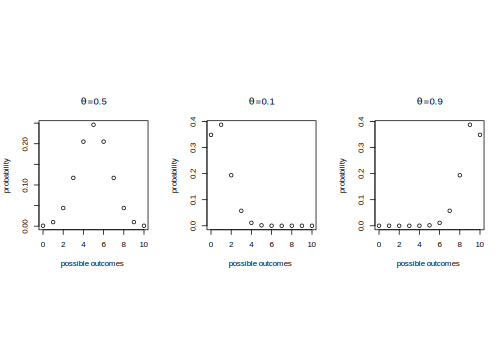
\includegraphics{Freq_CogSci_files/figure-latex/binomplot-1.pdf}
\caption{\label{fig:binomplot}Probability mass functions of a binomial distribution assuming 10 trials, with 50\%, 10\%, and 90\% probability of success.}
\end{figure}

\begin{rmdnote}
to-do bar or line graphs above, instead of points
\end{rmdnote}

The probability mass function for the binomial is written as follows.

\begin{equation}
\hbox{Binomial}(k|n,\theta) = 
\binom{n}{k} \theta^{k} (1-\theta)^{n-k}
\end{equation}

Here, \(n\) represents the total number of trials, \(k\) the number of successes, and \(\theta\) the probability of success. The term \(\binom{n}{k}\), pronounced n-choose-k, represents the number of ways in which one can choose \(k\) successes out of \(n\) trials. For example, 1 success out of 10 can occur in 10 possible ways: the very first trial could be a 1, the secone trial could be a 1, etc.
The term \(\binom{n}{k}\) expands to \(\frac{n!}{k!(n-k)!}\). In \texttt{R}, it is computed using the function \texttt{choose(n,k)}, with \(n\) and \(k\) representing positive integer values.

\hypertarget{the-mean-and-variance-of-the-binomial-distribution}{%
\subsection{The mean and variance of the Binomial distribution}\label{the-mean-and-variance-of-the-binomial-distribution}}

It is possible to analytically compute the mean and variance of the PMF associated with the Binomial random variable \(Y\). Without getting into the details of how these are derived mathematically, we just state here that the mean of \(Y\) (also called the expectation, conventionally written \(E[Y]\)) and variance of \(Y\) (written \(Var(Y)\)) of a Binomial distribution with parameter \(\theta\) and \(n\) trials are \(E[Y] = n\theta\) and \(Var(Y) = n\theta (1-\theta)\), respectively.

Of course, we always know \(n\) (because we decide on the number of trials ourselves), but in real experimental situations we never know the true value of \(\theta\). But \(\theta\) can be estimated from the data. From the observed data, we can compute the estimate of \(\theta\), \(\hat \theta=k/n\). The quantity \(\hat \theta\) is the observed proportion of successes, and is called the \textbf{maximum likelihood estimate} of the true (but unknown mean). Once we have estimated \(\theta\) in this way, we can also obtain an estimate (also a maximum likelihood estimate) of the variance by computing \(n\hat\theta (1-\hat\theta)\). These estimates are then used for statistical inference.

What does the term ``maximum likelihood estimate'' mean? The term \textbf{likelihood} refers to the value of the Binomial distribution function for a particular value of \(\theta\), once we have observed some data. For example, suppose you record \(n=10\) trials, and observe \(k=7\) successes. What is the probability of observing \(7\) successes out of \(10\)? We need the binomial distribution to compute this value:

\begin{equation}
\hbox{Binomial}(k=7|n=10,\theta) = 
\binom{10}{7} \theta^{7} (1-\theta)^{10-7}
\end{equation}

Once we have observed the data, both \(n\) and \(k\) are fixed. The only variable in the above equation now is \(\theta\): the above function is now only dependent on the value of \(\theta\). When the data are fixed, the probability mass function is only dependent on the value of the parameter \(\theta\), and is called a \textbf{likelihood function}. It is therefore often expressed as a function of \(\theta\):

\(p( y | \theta ) = p( k=7, n=10 | \theta) = \mathcal{L}(\theta)\)

The vertical bar notation above should be read as saying that, given some data \(y\) (which in the binomial case will be \(k\) ``successes'' in \(n\) trials), the function returns a value for different values of \(\theta\).

If we now plot this function for all possible values of \(\theta\), we get the plot shown in Figure \ref{fig:binomlik}.

\begin{figure}
\centering
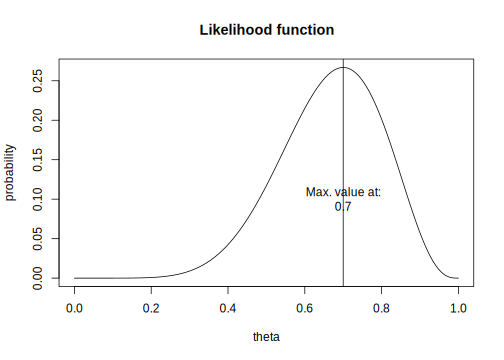
\includegraphics{Freq_CogSci_files/figure-latex/binomlik-1.pdf}
\caption{\label{fig:binomlik}The likelihood function for 7 successes out of 10.}
\end{figure}

\begin{rmdnote}
DS comment: do we want to show the code for computing all likelihood values? (maybe this comes later?)
\end{rmdnote}

What is important about this plot is that it shows that, given the data, the maximum point is at the point \(0.7\), which corresponds to the estimated mean using the formula shown above: \(k/n = 7/10\). Thus, the maximum likelihood estimate (MLE) gives us the most likely value that the parameter \(\theta\) given the data. It is crucial to note here that the phrase ``most likely'' here does not mean that the MLE from a \emph{particular} sample of data invariably gives us an accurate estimate of \(\theta\). For example, if we run our experiment for \(10\) trials and get \(1\) success out of \(10\), the MLE is \(0.10\). We could have happened to observe only one success out of ten even if the true \(\theta\) were \(0.5\). The MLE would however give an accurate estimate of the true parameter as \(n\) approaches infinity.

\hypertarget{what-information-does-a-probability-distribution-provide}{%
\subsection{What information does a probability distribution provide?}\label{what-information-does-a-probability-distribution-provide}}

What good is a probability mass function? We consider this question next.

\hypertarget{compute-the-probability-of-a-particular-outcome-discrete-case-only}{%
\subsubsection{Compute the probability of a particular outcome (discrete case only)}\label{compute-the-probability-of-a-particular-outcome-discrete-case-only}}

The Binomial distribution shown in Figure \ref{fig:binomplot} already shows the probability of each possible outcome under a different value for \(\theta\). In R, there is a built-in function that allows us to calculate the probability of \(k\) successes out of \(n\), given a particular value of \(k\) (this number constitutes our data), the number of trials \(n\), and given a particular value of \(\theta\); this is the \texttt{dbinom} function. For example, the probability of 5 successes out of 10 when \(\theta\) is 0.5 is:

\begin{Shaded}
\begin{Highlighting}[]
\KeywordTok{dbinom}\NormalTok{(}\DecValTok{5}\NormalTok{, }\DataTypeTok{size =} \DecValTok{10}\NormalTok{, }\DataTypeTok{prob =} \FloatTok{0.5}\NormalTok{)}
\end{Highlighting}
\end{Shaded}

\begin{verbatim}
## [1] 0.2461
\end{verbatim}

The probabilities of success when \(\theta\) is 0.1 or 0.9 can be computed by replacing 0.5 above by each of these probabilities. One can just do this by giving \texttt{dbinom} a vector of probabilities:

\begin{Shaded}
\begin{Highlighting}[]
\KeywordTok{dbinom}\NormalTok{(}\DecValTok{5}\NormalTok{, }\DataTypeTok{size =} \DecValTok{10}\NormalTok{, }\DataTypeTok{prob =} \KeywordTok{c}\NormalTok{(}\FloatTok{0.1}\NormalTok{, }\FloatTok{0.9}\NormalTok{))}
\end{Highlighting}
\end{Shaded}

\begin{verbatim}
## [1] 0.001488 0.001488
\end{verbatim}

\hypertarget{compute-the-cumulative-probability-of-k-or-less-more-than-k-successes}{%
\subsubsection{Compute the cumulative probability of k or less (more) than k successes}\label{compute-the-cumulative-probability-of-k-or-less-more-than-k-successes}}

Using the \texttt{dbinom} function, we can compute the cumulative probability of obtaining 1 or less, 2 or less successes etc. This is done through a simple summation procedure:

\begin{Shaded}
\begin{Highlighting}[]
\CommentTok{## the cumulative probability of obtaining 0, 1, or}
\CommentTok{## 2 successes out of 10, with theta=0.5:}
\KeywordTok{dbinom}\NormalTok{(}\DecValTok{0}\NormalTok{, }\DataTypeTok{size =} \DecValTok{10}\NormalTok{, }\DataTypeTok{prob =} \FloatTok{0.5}\NormalTok{) }\OperatorTok{+}\StringTok{ }\KeywordTok{dbinom}\NormalTok{(}\DecValTok{1}\NormalTok{, }\DataTypeTok{size =} \DecValTok{10}\NormalTok{, }
  \DataTypeTok{prob =} \FloatTok{0.5}\NormalTok{) }\OperatorTok{+}\StringTok{ }\KeywordTok{dbinom}\NormalTok{(}\DecValTok{2}\NormalTok{, }\DataTypeTok{size =} \DecValTok{10}\NormalTok{, }\DataTypeTok{prob =} \FloatTok{0.5}\NormalTok{)}
\end{Highlighting}
\end{Shaded}

\begin{verbatim}
## [1] 0.05469
\end{verbatim}

Mathematically, we could write the above summation as:

\begin{equation}
\sum_{k=0}^2 \binom{n}{k} \theta^{k} (1-\theta)^{n-k} 
\end{equation}

An alternative to the cumbersome addition in the R code above is this more compact statement, which closely mimics the above mathematical expression:

\begin{Shaded}
\begin{Highlighting}[]
\KeywordTok{sum}\NormalTok{(}\KeywordTok{dbinom}\NormalTok{(}\DecValTok{0}\OperatorTok{:}\DecValTok{2}\NormalTok{, }\DataTypeTok{size =} \DecValTok{10}\NormalTok{, }\DataTypeTok{prob =} \FloatTok{0.5}\NormalTok{))}
\end{Highlighting}
\end{Shaded}

\begin{verbatim}
## [1] 0.05469
\end{verbatim}

R has a built-in function called \texttt{pbinom} that does this summation for us. If we want to know the probability of \(2\) or less successes as in the above example, we can write:

\begin{Shaded}
\begin{Highlighting}[]
\KeywordTok{pbinom}\NormalTok{(}\DecValTok{2}\NormalTok{, }\DataTypeTok{size =} \DecValTok{10}\NormalTok{, }\DataTypeTok{prob =} \FloatTok{0.5}\NormalTok{, }\DataTypeTok{lower.tail =} \OtherTok{TRUE}\NormalTok{)}
\end{Highlighting}
\end{Shaded}

\begin{verbatim}
## [1] 0.05469
\end{verbatim}

The specification \texttt{lower.tail=TRUE} ensures that the summation goes from \(2\) to numbers smaller than \(2\) (which lie in the lower tail of the distribution in Figure \ref{fig:binomplot}). If we wanted to know what the probability is of obtaining \(2\) or more successes out of \(10\), we can set \texttt{lower.tail} to \texttt{FALSE}:

\begin{Shaded}
\begin{Highlighting}[]
\KeywordTok{pbinom}\NormalTok{(}\DecValTok{2}\NormalTok{, }\DataTypeTok{size =} \DecValTok{10}\NormalTok{, }\DataTypeTok{prob =} \FloatTok{0.5}\NormalTok{, }\DataTypeTok{lower.tail =} \OtherTok{FALSE}\NormalTok{)}
\end{Highlighting}
\end{Shaded}

\begin{verbatim}
## [1] 0.9453
\end{verbatim}

The cumulative distribution function or CDF can be plotted by computing the cumulative probabilities for any value \(k\) or less than \(k\), where \(k\) ranges from \(0\) to \(10\) in our running example. The CDF is shown in Figure \ref{fig:binomcdf}.

\begin{figure}
\centering
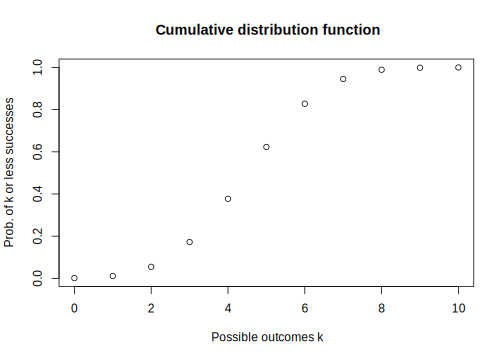
\includegraphics{Freq_CogSci_files/figure-latex/binomcdf-1.pdf}
\caption{\label{fig:binomcdf}The cumulative distribution function for a binomial distribution assuming 10 trials, with 50\% probability of success.}
\end{figure}

\hypertarget{compute-the-inverse-of-the-cumulative-distribution-function-the-quantile-function}{%
\subsubsection{Compute the inverse of the cumulative distribution function (the quantile function)}\label{compute-the-inverse-of-the-cumulative-distribution-function-the-quantile-function}}

We can also find out the value of the variable \(k\) (the quantile) such that the probability of obtaining \(k\) or less than \(k\) successes is some specific probability value \(p\). If we switch the x and y axes of Figure \ref{fig:binomcdf}, we obtain another very useful function, the inverse CDF.

The inverse of the CDF (known as the quantile function in R because it returns the quantile, the value k) is available in R as the function \texttt{qbinom}. The usage is as follows: to find out what the value \(k\) of the outcome is such that the probability of obtaining \(k\) or less successes is \(0.37\), type:

\begin{Shaded}
\begin{Highlighting}[]
\KeywordTok{qbinom}\NormalTok{(}\FloatTok{0.37}\NormalTok{, }\DataTypeTok{size =} \DecValTok{10}\NormalTok{, }\DataTypeTok{prob =} \FloatTok{0.5}\NormalTok{)}
\end{Highlighting}
\end{Shaded}

\begin{verbatim}
## [1] 4
\end{verbatim}

\hypertarget{generate-random-data-from-a-hboxbinomialntheta-distribution}{%
\subsubsection{\texorpdfstring{Generate random data from a \(\hbox{Binomial}(n,\theta)\) distribution}{Generate random data from a \textbackslash{}hbox\{Binomial\}(n,\textbackslash{}theta) distribution}}\label{generate-random-data-from-a-hboxbinomialntheta-distribution}}

We can generate random simulated data from a Binomial distribution by specifying the number of trials and the probability of success \(\theta\). In \texttt{R}, we do this as follows:

\begin{Shaded}
\begin{Highlighting}[]
\KeywordTok{rbinom}\NormalTok{(}\DecValTok{10}\NormalTok{, }\DataTypeTok{size =} \DecValTok{1}\NormalTok{, }\DataTypeTok{prob =} \FloatTok{0.5}\NormalTok{)}
\end{Highlighting}
\end{Shaded}

\begin{verbatim}
##  [1] 1 0 1 1 0 1 0 1 0 1
\end{verbatim}

The above code generates a sequences of \(1\)'s and \(0\)'s. Repeatedly run the above code; you will get different sequences each time. For each generated sequence, one can calculate the number of successes by just summing up the vector, or computing its mean and multiplying by the number of trials, here \(10\):

\begin{Shaded}
\begin{Highlighting}[]
\NormalTok{y <-}\StringTok{ }\KeywordTok{rbinom}\NormalTok{(}\DecValTok{10}\NormalTok{, }\DataTypeTok{size =} \DecValTok{1}\NormalTok{, }\DataTypeTok{prob =} \FloatTok{0.5}\NormalTok{)}
\KeywordTok{mean}\NormalTok{(y) }\OperatorTok{*}\StringTok{ }\DecValTok{10}
\end{Highlighting}
\end{Shaded}

\begin{verbatim}
## [1] 6
\end{verbatim}

\begin{Shaded}
\begin{Highlighting}[]
\KeywordTok{sum}\NormalTok{(y)}
\end{Highlighting}
\end{Shaded}

\begin{verbatim}
## [1] 6
\end{verbatim}

\hypertarget{continuous-random-variables-an-example-using-the-normal-distribution}{%
\section{Continuous random variables: An example using the Normal distribution}\label{continuous-random-variables-an-example-using-the-normal-distribution}}

We will now revisit the idea of a random variable using a continuous distribution. Imagine that you have a vector of reading time data \(y\) measured in milliseconds and coming from a Normal distribution. The probability density function (PDF) of the Normal distribution is defined as follows:

\begin{equation}
Normal(y|\mu,\sigma)=f(y)= \frac{1}{\sqrt{2\pi \sigma^2}} \exp \left(-\frac{(y-\mu)^2}{2\sigma^2} \right)
\end{equation}

Here, \(\mu\) is the mean, and \(\sigma\) is the standard deviation of the Normal distribution that the reading times have been sampled from.

We can visualize the Normal distribution for particular values of \(\mu\) and \(\sigma\) as a PDF (using \texttt{dnorm}), a CDF (using \texttt{pnorm}), and the inverse CDF (using \texttt{qnorm}). See Figure \ref{fig:normdistrn}.

In the figure, the PDF gives us the density for each possible value of our data \(y\); the CDF tells us the probability of observing a value like y or some value less than that (written: \(P(Y<y)\)); and the inverse CDF gives us the quantile \(y\) such that \(P(Y<y)\) is some specific value between 0 and 1. These are three different ways of looking at the same information.

\begin{figure}
\centering
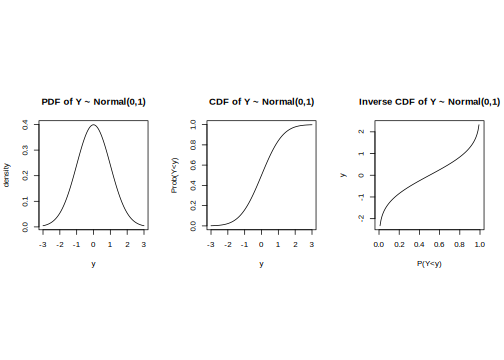
\includegraphics{Freq_CogSci_files/figure-latex/normdistrn-1.pdf}
\caption{\label{fig:normdistrn}The PDF, CDF, and inverse CDF for the \(Normal(\mu=0,\sigma=1)\).}
\end{figure}

One important fact about the normal distribution is that 95\% of the probability mass is covered by approximately plus/minus 1.96 times the standard deviation about the mean. Thus, the range \(\mu\pm 1.96\times \sigma\) will cover approximately 95\% of the area under the curve. We will approximate this by talking about \(\mu\pm 2\times \sigma\).

As in the discrete example, the PDF, CDF, and inverse of the CDF allow us to ask questions like:

\begin{itemize}
\tightlist
\item
  \textbf{What is the probability of observing values between \(a\) and \(b\) from a Normal distribution with mean \(\mu\) and standard deviation \(\sigma\)}? We can compute the probability of the random variable lying between 1 and minus infinity:
\end{itemize}

\begin{Shaded}
\begin{Highlighting}[]
\KeywordTok{pnorm}\NormalTok{(}\DecValTok{1}\NormalTok{, }\DataTypeTok{mean =} \DecValTok{0}\NormalTok{, }\DataTypeTok{sd =} \DecValTok{1}\NormalTok{) }\OperatorTok{-}\StringTok{ }\KeywordTok{pnorm}\NormalTok{(}\OperatorTok{-}\OtherTok{Inf}\NormalTok{, }\DataTypeTok{mean =} \DecValTok{0}\NormalTok{, }
  \DataTypeTok{sd =} \DecValTok{1}\NormalTok{)}
\end{Highlighting}
\end{Shaded}

\begin{verbatim}
## [1] 0.8413
\end{verbatim}

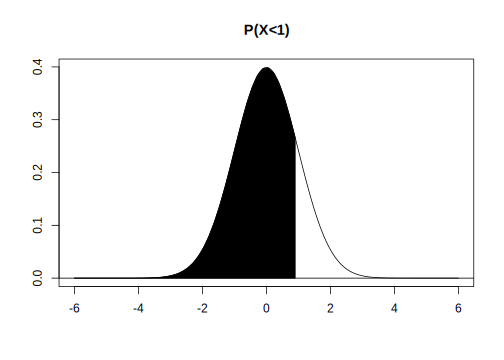
\includegraphics{Freq_CogSci_files/figure-latex/unnamed-chunk-10-1.pdf}

Notice here that the probability of any point value in a PDF is always 0. This is because the probability in a continuous probability distribution is the area under the curve, and the area at any point on the x-axis is always 0. The implication here is that we can only ask about probabilities between two different points; e.g., the probability that \(Y\) lies between \(a\) and \(b\), or \(P(a<Y<b)\). Also, notice that \(P(a<Y<b)\) and \(P(a\leq Y\leq b)\) will be the same probability, because of the fact that \(P(Y=a)\) or \(P(Y=b)\) both equal 0.

\begin{itemize}
\tightlist
\item
  \textbf{What is the quantile \(q\) such that the probability is \(p\) of observing that value \(q\) or something less (or more) than it}? For example, we can work out the quantile \(q\) such that the probability of observing \(q\) or something less than it is 0.975, in the Normal(500,100) distribution. Formally, we would write this as \(P(Y<a)\).
\end{itemize}

\begin{Shaded}
\begin{Highlighting}[]
\KeywordTok{qnorm}\NormalTok{(}\FloatTok{0.975}\NormalTok{, }\DataTypeTok{mean =} \DecValTok{500}\NormalTok{, }\DataTypeTok{sd =} \DecValTok{100}\NormalTok{)}
\end{Highlighting}
\end{Shaded}

\begin{verbatim}
## [1] 696
\end{verbatim}

The above output says that the probability that the random variable is less than \(q=695\) is 97.5\%.

\begin{itemize}
\tightlist
\item
  \textbf{Generating simulated data}. Given a vector of \(n\) independent and identically distributed data \(y\), i.e., given that each data point is being generated independently from \(Y \sim Normal(\mu,\sigma)\) for some values of the parameters, the maximum likelihood estimates for the expectation and variance are
\end{itemize}

\begin{equation}
\bar{y} =  \frac{\sum_{i=1}^n y_i}{n} 
\end{equation}

\begin{equation}
Var(y) = \frac{\sum_{i=1}^n (y_i-
\bar{y})^2}{n}
\end{equation}

For example, you could generate \(10\) data points using the \texttt{rnorm} function, and then compute the mean and variance from the simulated data:

\begin{Shaded}
\begin{Highlighting}[]
\NormalTok{y <-}\StringTok{ }\KeywordTok{rnorm}\NormalTok{(}\DecValTok{10}\NormalTok{, }\DataTypeTok{mean =} \DecValTok{500}\NormalTok{, }\DataTypeTok{sd =} \DecValTok{100}\NormalTok{)}
\KeywordTok{mean}\NormalTok{(y)}
\end{Highlighting}
\end{Shaded}

\begin{verbatim}
## [1] 482.2
\end{verbatim}

\begin{Shaded}
\begin{Highlighting}[]
\KeywordTok{var}\NormalTok{(y)}
\end{Highlighting}
\end{Shaded}

\begin{verbatim}
## [1] 13365
\end{verbatim}

Again, depending on the sample size, the sample mean and sample variance may or may not be close to the true values of the respective parameters, despite the fact that these are maximum likelihood estimates.

One other important detail about probability distributions is that one can have a joint distribution defined for more than one random variable. We consider this situation next, considering the continuous case only.

\hypertarget{bivariatemultivariate-distributions}{%
\section{Bivariate/multivariate distributions}\label{bivariatemultivariate-distributions}}

So far, we have only discussed univariate distributions. It is also possible to specify distributions with two or more dimensions. For example, consider the bivariate case:
two normal random variables \(U_0\) and \(U_1\), each of which coming from, for example, a Normal(0,1) distribution, with some correlation \(\rho\) between the random variables.

A bivariate distribution for two random variables \(U_0\) and \(U_1\), each of which comes from a normal distribution, is expressed in terms of the means and standard deviations of each of the two distributions, and the correlation \(\rho\) between them. The standard deviations and correlation are expressed in a special form of a \(2\times 2\) matrix called a variance covariance matrix \(\Sigma\). If \(\rho_u\) is the correlation between the two random variables, and \(\sigma _{u0}\) and \(\sigma _{u1}\) the respective standard deviations, the variance covariance matrix is written as:

\begin{equation}\label{eq:covmatfoundations}
\Sigma
=
\begin{pmatrix}
\sigma _{u0}^2  & \rho _{u}\sigma _{u0}\sigma _{u1}\\
\rho _{u}\sigma _{u0}\sigma _{u1}    & \sigma _{u1}^2\\
\end{pmatrix}
\end{equation}

The off-diagonals of this matrix contain the covariance between \(U_0\) and \(U_1\).

The joint distribution of \(U_0\) and \(U_1\) is defined as follows:

\begin{equation}\label{eq:jointpriordistfoundations}
\begin{pmatrix}
  U_0 \\ 
  U_1 \\
\end{pmatrix}
\sim 
\mathcal{N}_2 \left(
\begin{pmatrix}
  0 \\
  0 \\
\end{pmatrix},
\Sigma
\right)
\end{equation}

A visualization will help. The figure below shows a bivariate distribution with correlation zero, a positive and a negative correlation.

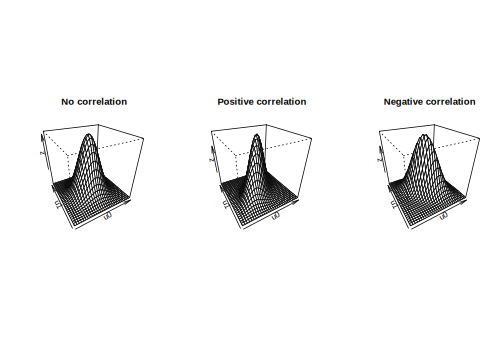
\includegraphics{Freq_CogSci_files/figure-latex/unnamed-chunk-11-1.pdf}

In this book, we will make use of such multivariate distributions a lot, and it will soon become important to know how to generate simulated bivariate data that is correlated. Suppose we want to generate 100 correlated pairs of data, with correlation \(\rho=0.6\). The two random variables have mean 0, and standard deviations 5 and 10 respectively.

Here is how we would generate such data. First, define a variance covariance matrix; then, use the multivariate analog of the \texttt{rnorm} function, \texttt{mvrnorm}, to generate \(100\) data-points.

\begin{Shaded}
\begin{Highlighting}[]
\KeywordTok{library}\NormalTok{(MASS)}
\CommentTok{## define a variance-covariance matrix:}
\NormalTok{Sigma <-}\StringTok{ }\KeywordTok{matrix}\NormalTok{(}\KeywordTok{c}\NormalTok{(}\DecValTok{5}\OperatorTok{^}\DecValTok{2}\NormalTok{, }\DecValTok{5} \OperatorTok{*}\StringTok{ }\DecValTok{10} \OperatorTok{*}\StringTok{ }\FloatTok{0.6}\NormalTok{, }\DecValTok{5} \OperatorTok{*}\StringTok{ }\DecValTok{10} \OperatorTok{*}\StringTok{ }\FloatTok{0.6}\NormalTok{, }
  \DecValTok{10}\OperatorTok{^}\DecValTok{2}\NormalTok{), }\DataTypeTok{byrow =} \OtherTok{FALSE}\NormalTok{, }\DataTypeTok{ncol =} \DecValTok{2}\NormalTok{)}
\CommentTok{## generate data:}
\NormalTok{u <-}\StringTok{ }\KeywordTok{mvrnorm}\NormalTok{(}\DataTypeTok{n =} \DecValTok{100}\NormalTok{, }\DataTypeTok{mu =} \KeywordTok{c}\NormalTok{(}\DecValTok{0}\NormalTok{, }\DecValTok{0}\NormalTok{), }\DataTypeTok{Sigma =}\NormalTok{ Sigma)}
\KeywordTok{head}\NormalTok{(u)}
\end{Highlighting}
\end{Shaded}

\begin{verbatim}
##        [,1]    [,2]
## [1,] -0.453   5.233
## [2,]  4.222   6.372
## [3,]  3.602  10.269
## [4,] -6.151  -4.627
## [5,] -3.412   6.823
## [6,] -2.036 -18.415
\end{verbatim}

A plot confirms that the data are positively correlated.

\begin{Shaded}
\begin{Highlighting}[]
\KeywordTok{plot}\NormalTok{(u[, }\DecValTok{1}\NormalTok{], u[, }\DecValTok{2}\NormalTok{])}
\end{Highlighting}
\end{Shaded}

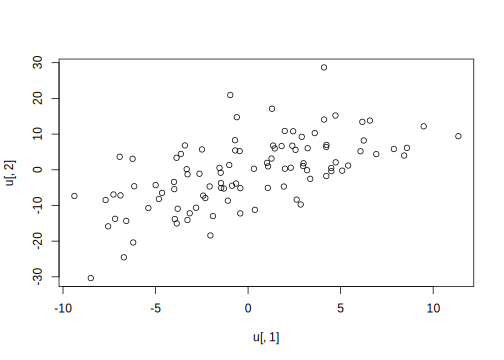
\includegraphics{Freq_CogSci_files/figure-latex/unnamed-chunk-13-1.pdf}

As an exercise, try changing the correlation to \(0\) or to \(-0.6\), and then plot the bivariate distribution that results.

One final useful thing to notice about the variance-covariance matrix is that it can be decomposed into the component standard deviations and an underlying correlation matrix. For example, consider the matrix above:

\begin{Shaded}
\begin{Highlighting}[]
\NormalTok{Sigma}
\end{Highlighting}
\end{Shaded}

\begin{verbatim}
##      [,1] [,2]
## [1,]   25   30
## [2,]   30  100
\end{verbatim}

One can decompose the matrix as follows. The matrix can be seen as the product of a diagonal matrix of the standard deviations and the correlation matrix:

\begin{Shaded}
\begin{Highlighting}[]
\CommentTok{## sds:}
\NormalTok{(sds <-}\StringTok{ }\KeywordTok{c}\NormalTok{(}\DecValTok{5}\NormalTok{, }\DecValTok{10}\NormalTok{))}
\end{Highlighting}
\end{Shaded}

\begin{verbatim}
## [1]  5 10
\end{verbatim}

\begin{Shaded}
\begin{Highlighting}[]
\CommentTok{## diagonal matrix:}
\NormalTok{(sd_diag <-}\StringTok{ }\KeywordTok{diag}\NormalTok{(sds))}
\end{Highlighting}
\end{Shaded}

\begin{verbatim}
##      [,1] [,2]
## [1,]    5    0
## [2,]    0   10
\end{verbatim}

\begin{Shaded}
\begin{Highlighting}[]
\CommentTok{## correlation matrix:}
\NormalTok{(corrmatrix <-}\StringTok{ }\KeywordTok{matrix}\NormalTok{(}\KeywordTok{c}\NormalTok{(}\DecValTok{1}\NormalTok{, }\FloatTok{0.6}\NormalTok{, }\FloatTok{0.6}\NormalTok{, }\DecValTok{1}\NormalTok{), }\DataTypeTok{ncol =} \DecValTok{2}\NormalTok{))}
\end{Highlighting}
\end{Shaded}

\begin{verbatim}
##      [,1] [,2]
## [1,]  1.0  0.6
## [2,]  0.6  1.0
\end{verbatim}

Given these two matrices, one can reassemble the variance covariance matrix:

\begin{Shaded}
\begin{Highlighting}[]
\NormalTok{sd_diag }\OperatorTok\StringTok{ }\NormalTok{corrmatrix }\OperatorTok\StringTok{ }\NormalTok{sd_diag}
\end{Highlighting}
\end{Shaded}

\begin{verbatim}
##      [,1] [,2]
## [1,]   25   30
## [2,]   30  100
\end{verbatim}

There is a built-in convenience function, sdcor3cov in the SIN package that does this calculation, taking the vector of standard deviatios (not the diagonal matrix) and the correlation matrix to yield the variance covariance matrix:

\begin{Shaded}
\begin{Highlighting}[]
\NormalTok{SIN}\OperatorTok{::}\KeywordTok{sdcor2cov}\NormalTok{(}\DataTypeTok{stddev =}\NormalTok{ sds, }\DataTypeTok{corr =}\NormalTok{ corrmatrix)}
\end{Highlighting}
\end{Shaded}

\begin{verbatim}
##      [,1] [,2]
## [1,]   25   30
## [2,]   30  100
\end{verbatim}

We will be using this function a lot when simulating data from linear mixed models.

\hypertarget{summary-of-useful-r-functions-relating-to-univariate-distributions}{%
\section{Summary of useful R functions relating to univariate distributions}\label{summary-of-useful-r-functions-relating-to-univariate-distributions}}

Table \ref{tab:dpqrfunctions} summarizes the different functions relating to univariate PMFs and PDFs, using the Binomial and Normal as examples.

\begin{longtable}[]{@{}lcc@{}}
\caption{\label{tab:dpqrfunctions} Important R functions relating to two univariate random variables, the Normal and the Binomial.}\tabularnewline
\toprule
& Discrete & Continuous\tabularnewline
\midrule
\endfirsthead
\toprule
& Discrete & Continuous\tabularnewline
\midrule
\endhead
Example: & Binomial(n,\(\theta\)) & Normal(\(\mu,\sigma\))\tabularnewline
Likelihood function & dbinom & dnorm\tabularnewline
Prob Y=y & dbinom & always 0\tabularnewline
Prob \(Y\geq y, Y\leq y, y_1<Y<y_2\) & pbinom & pnorm\tabularnewline
Inverse CDF & qbinom & qnorm\tabularnewline
Generate simulated data & rbinom & rnorm\tabularnewline
\bottomrule
\end{longtable}

Other distributions, such as the t-distribution, the Uniform, Exponential, Gamma, etc. Beta, etc., have their own set of d-p-q-r functions in R. The appendix summarizes the properties of the distributions that we will need in this book.

\hypertarget{summary-of-random-variable-theory}{%
\section{*Summary of random variable theory}\label{summary-of-random-variable-theory}}

We can summarize the above informal concepts very compactly if we re-state them in mathematical form. A mathematical statement has the advantage not only of brevity but also of reducing ambiguity.

Formally, a random variable \(Y\) is defined as a function from a sample space of possible outcomes \(S\) to the real number system:

\begin{equation}
Y : S \rightarrow \mathbb{R}
\end{equation}

The random variable associates to each outcome \(\omega \in S\) exactly one number \(Y(\omega) = y\). \(S_Y\) is all the \(y\)'s (all the possible values of \(Y\), the support of \(Y\)). I.e., \(y \in S_Y\).

Every random variable \(Y\) has associated with it a probability mass (distribution) function (PMF, PDF). I.e., PMF is used for discrete distribu tions and PDF for continuous distributions. The PMF/PDF maps every element of \(S_Y\) to a value between 0 and 1.

\begin{equation}
p_Y : S_Y \rightarrow [0, 1] 
\end{equation}

Probability mass functions (discrete case) and probability density functions (continuous case) are functions that assign probabilities or relative frequencies to all events in a sample space.

The expression

\begin{equation}
 Y \sim f(\cdot)
\end{equation}

\noindent
will be used to mean that the random variable \(Y\) has pdf/pmf \(f(\cdot)\).
For example, if we say that \(Y \sim Binomial(n,\theta)\), then we are asserting that the PMF is:

\begin{equation}
\hbox{Binomial}(k|n,\theta) = 
\binom{n}{k} \theta^{k} (1-\theta)^{n-k}
\end{equation}

If we say that \(Y\sim Normal(\mu,\sigma)\), we are asserting that the PDF is

\begin{equation}
Normal(y|\mu,\sigma)= \frac{1}{\sqrt{2\pi \sigma^2}} \exp \left(-\frac{y-\mu)^2}{2\sigma^2} \right)
\end{equation}

The \textbf{cumulative distribution function} or CDF is defined as follows:

For discrete distributions, the probability that \(Y\) is less than \(a\) is written:

\begin{equation}
P(Y<a) = F(Y<a) =\sum_{-\infty}^{a} f(y)
\end{equation}

For continuous distributions, the summation symbol \(\sum\) above becomes the summation symbol for the continuous case, which is the integral \(\int\). The upper and lower bounds are marked by adding a subscript and a superscript on the integral. For example, if we want the area under the curve between points a and b for some function \(f(y)\), we write \(\int_b^a f(y)\, dy\). So, if we want the probability that \(Y\) is less than \(a\), we would write:

\begin{equation}
P(Y<a) = F(Y<a) =\int_{-\infty}^{a} f(y)\, dy
\end{equation}

The above integral is simply summing up the area under the curve between the points \(-\infty\) and \(a\); this gives us the probability of observing \(a\) or a value smaller than \(a\).

A final point here is that we can go back and forth between the PDF and the CDF. If the PDF is \(f(y)\), then the CDF that allows us to compute quantities like \(P(Y<b)\) is just the integral \(F(Y<b)=\int_{-\infty}^b f(y)\, dy\). If we differentiate the CDF, we get the PDF back: \(d(F(y))/dy=f(y)\).

\hypertarget{further-reading}{%
\section{Further reading}\label{further-reading}}

A quick review of the mathematical foundations needed for statistics is available in the short book by \citet{fox2009mathematical}. \citet{morin2016probability} and \citet{blitzstein2014introduction} are accessible introductions to probability theory. \citet{kerns} contains a very well-written general introduction to random variable theory, but assumes the reader knows the basics of calculus.

\hypertarget{sec:Foundationsexercises}{%
\section{Exercises}\label{sec:Foundationsexercises}}

\hypertarget{sec:Foundationsexercisespnorm}{%
\subsection{\texorpdfstring{Practice using the \texttt{pnorm} function}{Practice using the pnorm function}}\label{sec:Foundationsexercisespnorm}}

\hypertarget{sec:FoundationsexercisespnormPart1}{%
\subsubsection{Part 1}\label{sec:FoundationsexercisespnormPart1}}

Given a normal distribution with mean \texttt{73} and standard deviation \texttt{101}, use the pnorm function to calculate the probability of obtaining values between \texttt{30} and \texttt{-47} from this distribution.

\hypertarget{sec:FoundationsexercisespnormPart2}{%
\subsubsection{Part 2}\label{sec:FoundationsexercisespnormPart2}}

Calculate the following probabilities.
Given a normal distribution with mean \texttt{50} and standard deviation \texttt{3}, what is the probability of getting

\begin{itemize}
\tightlist
\item
  a score of \texttt{40} or less
\item
  a score of \texttt{40} or more
\item
  a score of \texttt{59} or more
\end{itemize}

\hypertarget{sec:FoundationsexercisespnormPart3}{%
\subsubsection{Part 3}\label{sec:FoundationsexercisespnormPart3}}

Given a normal distribution with mean \texttt{55} and standard deviation \texttt{6}, what is the probability of getting

\begin{itemize}
\tightlist
\item
  a score of \texttt{50} or less.
\item
  a score between \texttt{52} and \texttt{58}.
\item
  a score of \texttt{mu+1} or more.
\end{itemize}

\hypertarget{sec:Foundationsexercisesqnorm}{%
\subsection{\texorpdfstring{Practice using the \texttt{qnorm} function}{Practice using the qnorm function}}\label{sec:Foundationsexercisesqnorm}}

\hypertarget{sec:FoundationsexercisesqnormPart1}{%
\subsubsection{Part 1}\label{sec:FoundationsexercisesqnormPart1}}

Consider a normal distribution with mean 1 and standard deviation 1.

Compute the lower and upper boundaries such that:

\begin{itemize}
\tightlist
\item
  the area (the probability) to the left of the lower boundary is \texttt{0.46}.
\item
  the area (the probability) to the left of the upper boundary is \texttt{0.81}.
\end{itemize}

\hypertarget{sec:FoundationsexercisesqnormPart2}{%
\subsubsection{Part 2}\label{sec:FoundationsexercisesqnormPart2}}

Given a normal distribution with mean \texttt{59.061} and standard deviation \texttt{0.673}. There exist two quantiles, the lower quantile q1 and the upper quantile q2, that are equidistant from the mean \texttt{59.061}, such that the area under the curve of the Normal probability between q1 and q2 is \texttt{85}\%. Find q1 and q2.

\hypertarget{sec:Foundationsexercisesqt}{%
\subsection{\texorpdfstring{Practice using \texttt{qt}}{Practice using qt}}\label{sec:Foundationsexercisesqt}}

Take an independent random sample of size \texttt{157} from a normal distribution
with mean \texttt{170}, and standard deviation \texttt{37}. Next, we are going to pretend we don't know the population parameters (the mean and standard deviation). We compute the MLEs of the mean and standard deviation using the data and get the sample mean \texttt{171.138} and the sample standard deviation \texttt{35.223}.

\begin{itemize}
\tightlist
\item
  Compute the estimated standard error using the sample standard deviation provided above.
\item
  What are your degrees of freedom for the relevant t-distribution?
\item
  Calculate the \textbf{absolute} critical t-value for a 95\% confidence interval using the relevant degrees of freedom you just wrote above.
\item
  Next, compute the lower bound of the 95\% confidence interval using the estimated standard error and the critical t-value.
\item
  Finally, compute the upper bound of the 95\% confidence interval using the estimated standard error and the critical t-value.
\end{itemize}

\hypertarget{sec:FoundationsexercisesMLE1}{%
\subsection{Maximum likelihood estimation 1}\label{sec:FoundationsexercisesMLE1}}

Given the data point \texttt{16.655}.
The function \texttt{dnorm} gives the likelihood given a data point (or multiple data points) and a value for the mean and the standard deviation (sd). Using \texttt{dnorm}, compute

\begin{itemize}
\tightlist
\item
  the likelihood of the data point \texttt{16.655} assuming a mean of \texttt{12} and standard deviation 5.
\item
  the likelihood of the data point \texttt{16.655} assuming a mean of \texttt{11} and standard deviation 5.
\item
  the likelihood of the data point \texttt{16.655} assuming a mean of \texttt{10} and standard deviation 5.
\item
  the likelihood of the data point \texttt{16.655} assuming a mean of \texttt{9} and standard deviation 5.
\end{itemize}

\hypertarget{sec:FoundationsexercisesMLE2}{%
\subsection{Maximum likelihood estimation 2}\label{sec:FoundationsexercisesMLE2}}

You are given \(10\) independent and identically distributed data points that are assumed to come from a Normal distribution with unknown mean and unknown standard deviation:

\begin{Shaded}
\begin{Highlighting}[]
\NormalTok{x}
\end{Highlighting}
\end{Shaded}

\begin{verbatim}
##  [1] 513 491 501 500 494 490 500 507 515 481
\end{verbatim}

The function \texttt{dnorm} gives the likelihood given multiple data points and a value for the mean and the standard deviation. The log-likelihood can be computed by typing \texttt{dnorm(...,log=TRUE)}.

The product of the likelihoods for two independent data points can be computed like this: Suppose we have two independent and identically distributed data points 5 and 10. Then, assuming that the Normal distribution they come from has mean 10 and standard deviation 2, the joint likelihood of these is:

\begin{Shaded}
\begin{Highlighting}[]
\KeywordTok{dnorm}\NormalTok{(}\DecValTok{5}\NormalTok{, }\DataTypeTok{mean =} \DecValTok{10}\NormalTok{, }\DataTypeTok{sd =} \DecValTok{2}\NormalTok{) }\OperatorTok{*}\StringTok{ }\KeywordTok{dnorm}\NormalTok{(}\DecValTok{10}\NormalTok{, }\DataTypeTok{mean =} \DecValTok{10}\NormalTok{, }
  \DataTypeTok{sd =} \DecValTok{2}\NormalTok{)}
\end{Highlighting}
\end{Shaded}

\begin{verbatim}
## [1] 0.001748
\end{verbatim}

It is easier to do this on the log scale, because then one can add instead of multiplying. This is because \(\log(x\times y)= \log(x) + \log(y)\). For example:

\begin{Shaded}
\begin{Highlighting}[]
\KeywordTok{log}\NormalTok{(}\DecValTok{2} \OperatorTok{*}\StringTok{ }\DecValTok{3}\NormalTok{)}
\end{Highlighting}
\end{Shaded}

\begin{verbatim}
## [1] 1.792
\end{verbatim}

\begin{Shaded}
\begin{Highlighting}[]
\KeywordTok{log}\NormalTok{(}\DecValTok{2}\NormalTok{) }\OperatorTok{+}\StringTok{ }\KeywordTok{log}\NormalTok{(}\DecValTok{3}\NormalTok{)}
\end{Highlighting}
\end{Shaded}

\begin{verbatim}
## [1] 1.792
\end{verbatim}

So the joint log likelihood of the two data points is:

\begin{Shaded}
\begin{Highlighting}[]
\KeywordTok{dnorm}\NormalTok{(}\DecValTok{5}\NormalTok{, }\DataTypeTok{mean =} \DecValTok{10}\NormalTok{, }\DataTypeTok{sd =} \DecValTok{2}\NormalTok{, }\DataTypeTok{log =} \OtherTok{TRUE}\NormalTok{) }\OperatorTok{+}\StringTok{ }\KeywordTok{dnorm}\NormalTok{(}\DecValTok{10}\NormalTok{, }
  \DataTypeTok{mean =} \DecValTok{10}\NormalTok{, }\DataTypeTok{sd =} \DecValTok{2}\NormalTok{, }\DataTypeTok{log =} \OtherTok{TRUE}\NormalTok{)}
\end{Highlighting}
\end{Shaded}

\begin{verbatim}
## [1] -6.349
\end{verbatim}

Even more compactly:

\begin{Shaded}
\begin{Highlighting}[]
\KeywordTok{sum}\NormalTok{(}\KeywordTok{dnorm}\NormalTok{(}\KeywordTok{c}\NormalTok{(}\DecValTok{5}\NormalTok{, }\DecValTok{10}\NormalTok{), }\DataTypeTok{mean =} \DecValTok{10}\NormalTok{, }\DataTypeTok{sd =} \DecValTok{2}\NormalTok{, }\DataTypeTok{log =} \OtherTok{TRUE}\NormalTok{))}
\end{Highlighting}
\end{Shaded}

\begin{verbatim}
## [1] -6.349
\end{verbatim}

\begin{itemize}
\tightlist
\item
  Given the 10 data points above, calculate the maximum likelihood estimate (MLE) of the expectation.
\item
  The sum of the log-likelihoods of the data-points x, using as the mean the MLE from the sample, and standard deviation 5.
\item
  What is the sum of the log-likelihood if the mean used to compute the log-likelihood is \texttt{497.2}?
\item
  Which value for the mean, the MLE or \texttt{497.2}, gives the higher log-likelihood?
\end{itemize}

\hypertarget{sec:Foundationsexercisesbivar}{%
\subsection{Generating bivariate data}\label{sec:Foundationsexercisesbivar}}

Generate 50 data points from two random variables X and Y, where \(X\sim Normal(50,100)\) and \(Y\sim Normal(100,20)\). The correlation between the random variables is 0.7. Plot the simulated data points from Y against those from X.

\hypertarget{sec:Foundationsexercisesmultivar}{%
\subsection{Generating multivariate data}\label{sec:Foundationsexercisesmultivar}}

The bivariate case can be generalized to more than two dimensions.
Generate 50 data points from three random variables X, Y, and Z, where \(X\sim Normal(50,100)\), \(Y\sim Normal(100,20)\), and \(Z\sim Normal(200,50)\). The correlation between the random variables X and Y is 0.5, between X and Z is 0.2, an between Y and Z is 0.7. Here, you will have to define a \(3\times 3\) variance covariance matrix, with the pairwise covariances in the off-diagonals. Plot the simulated data points as two-dimensional figures: Y against X, Y against Z, and X against Z.

\hypertarget{hypothetical-repeated-sampling-and-the-t-test}{%
\chapter{Hypothetical repeated sampling and the t-test}\label{hypothetical-repeated-sampling-and-the-t-test}}

This chapter introduces some of the foundational ideas behind hypothesis testing in the frequentist framework. The key idea if that of hypothetical repeated sampling. When we fit a model to a given data-set, we are assuming that this is one of potentially infinite numbers of exact repetitions of an experiment. We leverage some amazing properties of these exact repetitions in order to draw inferences from our particular data. The key idea to understand here is the central limit theorem, to which we turn next.

\hypertarget{the-central-limit-theorem-using-simulation}{%
\section{The central limit theorem using simulation}\label{the-central-limit-theorem-using-simulation}}

Suppose we collect some data, which can be represented by a vector \(y\); this is a \emph{single sample}. Given data \(y\), and assuming for concreteness that the underlying likelihood is a \(Normal(\mu=500,\sigma=100)\), the sample mean and standard deviation, \(\bar{y}\) and \(s\) give us an estimate of the unknown parameters mean \(\mu\) and the standard deviation \(\sigma\) that are assumed to generate the data. Figure \ref{fig:normalsample} shows the distribution of a particular sample, where the number of data points is \(n=1000\). Note that in this example the parameters are specified by us, so they are not unknown; in a real data-collection situation, the sample mean and standard deviation are all we have as estimates of the parameters.

\begin{figure}
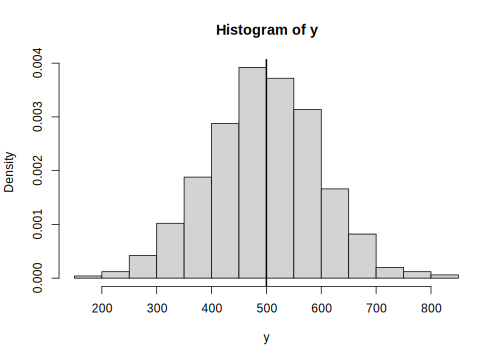
\includegraphics[width=0.75\linewidth]{Freq_CogSci_files/figure-latex/normalsample-1} \caption{A sample of data y, from the distribution  Normal(500,100).}\label{fig:normalsample}
\end{figure}

Suppose now that you had not a single sample of size 1000 but many repeated samples. This isn't something one can normally do in real life; we often run a single experiment or, at most, repeat the same experiment once. However, one can simulate repeated sampling easily within R. Let us take 100 repeated samples like the one above, and save the samples in a matrix containing n=1000 rows and 100 columns, each column representing an experiment:

\begin{Shaded}
\begin{Highlighting}[]
\NormalTok{mu <-}\StringTok{ }\DecValTok{500}
\NormalTok{sigma <-}\StringTok{ }\DecValTok{100}
\CommentTok{## number of experiments:}
\NormalTok{k <-}\StringTok{ }\DecValTok{100}
\CommentTok{## store for data:}
\NormalTok{y_matrix <-}\StringTok{ }\KeywordTok{matrix}\NormalTok{(}\KeywordTok{rep}\NormalTok{(}\OtherTok{NA}\NormalTok{, n }\OperatorTok{*}\StringTok{ }\NormalTok{k), }\DataTypeTok{ncol =}\NormalTok{ k)}
\ControlFlowTok{for}\NormalTok{ (i }\ControlFlowTok{in} \DecValTok{1}\OperatorTok{:}\NormalTok{k) \{}
  \CommentTok{## expt result with sample size n:}
\NormalTok{  y_matrix[, i] <-}\StringTok{ }\KeywordTok{rnorm}\NormalTok{(n, }\DataTypeTok{mean =}\NormalTok{ mu, }\DataTypeTok{sd =}\NormalTok{ sigma)}
\NormalTok{\}}
\end{Highlighting}
\end{Shaded}

Now, if we compute the means \(\bar{y}_k\) of \emph{each} of the \(k=1,\dots,100\) experiments we just carried out, if certain conditions are met, these means will be normally distributed, with mean \(\mu\) and standard deviation \(\sigma/\sqrt{n}\). To understand this point, it is useful to first visualize the distribution of means and graphically summarize this standard deviation, which confusingly is called \emph{standard error}.

\begin{Shaded}
\begin{Highlighting}[]
\CommentTok{## compute means from each replication:}
\NormalTok{y_means <-}\StringTok{ }\KeywordTok{colMeans}\NormalTok{(y_matrix)}
\CommentTok{## the mean and sd (=standard error) of the means}
\KeywordTok{mean}\NormalTok{(y_means)}
\end{Highlighting}
\end{Shaded}

\begin{verbatim}
## [1] 499.6
\end{verbatim}

\begin{Shaded}
\begin{Highlighting}[]
\KeywordTok{sd}\NormalTok{(y_means)}
\end{Highlighting}
\end{Shaded}

\begin{verbatim}
## [1] 3.053
\end{verbatim}

\begin{figure}
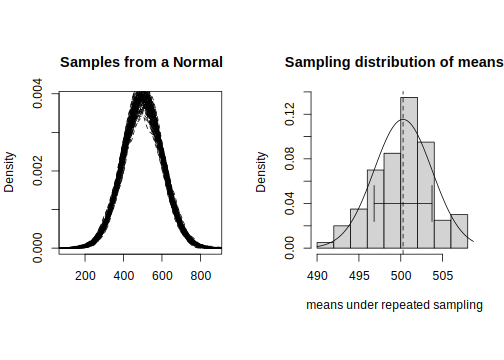
\includegraphics[width=0.75\linewidth]{Freq_CogSci_files/figure-latex/sdsmnormal-1} \caption{Sampling from a normal distribution (left); and the sampling distribution of the means under repeated sampling (right). The right-hand plot shows an overlaid normal distribution, and the standard deviation (standard error) as error bars.}\label{fig:sdsmnormal}
\end{figure}

The sampling distribution of means has a normal distribution provided two conditions are met: (a) the sample size should be large enough, and (b) \(\mu\) and \(\sigma\) are defined for the probability density or mass function that generated the data. This fact is called the \textbf{central limit theorem} (CLT). The significance of the CLT for us as researchers is that from the summary statistics computed from a \emph{single} sample, we can obtain an estimate of this distribution of means: \(Normal(\bar{y},s/\sqrt{n})\).

The statement that the sampling distribution of the means will be normal, with mean \(\mu\) and standard deviation \(\sigma/\sqrt{n}\), can be derived formally through a surprisingly simple application of random variable theory. Suppose we gather independent and identically distributed data \(y_1, \dots, y_n\), each of which is generated by a random variable \(Y\sim Normal(\mu,\sigma)\).

When we compute the mean \(\bar{y}\) for each sample, we are assuming that each of the means is coming from a random variable \(\bar{Y}\), which is just a linear combination of values generated by instances of the random variable \(Y\), which itself has a pdf with mean (expectation) \(\mu\) and variance \(\sigma^2\):

\begin{equation}
\bar{Y}=\frac{1}{n} \sum_{i=1}^n Y = \frac{1}{n}Y_1 + \dots + \frac{1}{n}Y_n
 \end{equation}

So, the expectation of \(\bar{Y}\) is

\begin{equation}
\begin{split}
E[\bar{Y}] =& E[\frac{1}{n}Y_1 + \dots + \frac{1}{n}Y_n]\\
=& \frac{1}{n} (E[Y] + \dots + E[Y])\\
=& \frac{1}{n} (\mu + \dots + \mu)\\
=& \frac{1}{n} n\mu \\
=& \mu \\
\end{split}
\end{equation}

And the variance of \(\bar{Y}\) is

\begin{equation}
\begin{split}
Var(\bar{Y}) =& Var(\frac{1}{n}Y_1 + \dots + \frac{1}{n}
Y_n)\\
=& \frac{1}{n} [Var(Y_1 + \dots + Y_n)]\\
=& \frac{1}{n^2} Var(Y_1 + \dots + Y_n)\\
\end{split}
\end{equation}

The last line above arises because the variance of a random variable \(Z\) multiplied by a constant \(a\), \(Var(aZ)\) is \(a^2 Var(Z)\). Here, \(a=1/n\), so \(a^2 = 1/n^2\).
Because \(Y_1,\dots,Y_n\) are independent, we can compute the variance \(Var(Y_1 + \dots + Y_n)\) by using the fact that the variance of the sum of independent random variables is the sum of their variances. This fact gives us:

\begin{equation} \label{sdsmderivation}
\begin{split}
\frac{1}{n^2} Var(Y_1 + \dots + Y_n) =& \frac{1}{n^2} (Var(Y) + \dots + Var(Y))\\
=&  \frac{1}{n^2}  n Var(Y)\\
=&  \frac{1}{n}  Var(Y)\\
=&  \frac{\sigma^2}{n}\\
\end{split}
\end{equation}

This derives the above result that the expectation (i.e., the mean) and variance of the sampling distribution of the sample means are

\begin{equation}
E[\bar{Y}] = \mu \quad Var(\bar{Y}) = \frac{\sigma^2}{n}
\end{equation}

The Central Limit Theorem, not proved here (for a proof, see p.~267 of \citet{millermiller}) can be summarized as follows.

\textbf{Central Limit Theorem}

Let \(f(Y)\) be the pdf of a random variable \(Y\), and assume that the pdf has mean \(\mu\) and variance \(\sigma^2\). Then:

\begin{equation}
\bar{Y} \sim Normal(\mu,\sigma^2/n) \quad  E[Y]=\mu,Var(Y)=\sigma^2 \quad \hbox{ when n is large}
\end{equation}

For us, the practical implication of this result is huge. From a \emph{single} sample \(y_1,\dots, y_n\), we can derive the distribution of \emph{hypothetical} sample means under repeated sampling. That is, it becomes possible to say something about what the plausible and implausible values of the sample mean are under repeated sampling. This is the basis for all hypothesis testing and statistical inference in the frequentist framework that we will look at in this book.

Sometimes the central limit theorem is misunderstood to imply that the distribution that is assumed to generate the data is always going to be normal. It is important to understand that there are two distributions we are talking about here. First, there is the distribution that the data were generated from; this need not be normal. For example, you could get data from a Normal, Exponential, Gamma, or other distribution. Second, there is the sampling distribution of the \emph{sample mean} under repeated sampling. It is the sampling distribution that the central limit theorem is about, not the distribution that generated the data.

\hypertarget{three-examples-of-the-sampling-distribution}{%
\section{Three examples of the sampling distribution}\label{three-examples-of-the-sampling-distribution}}

In the above discussion, the underlying pdf we sampled from above was a normal distribution. However, it need not be. Consider two examples: the underlying pdf is an Exponential or a Gamma distribution.

The Exponential distribution has a parameter \(\lambda\) (parameterized in \texttt{R} as a \texttt{rate}, \(1/\lambda\)); its mean is \(\lambda\) and its variance is \(1/\lambda^2\). The sampling distribution is normal, even though the underlying distribution is an Exponential.

\begin{figure}
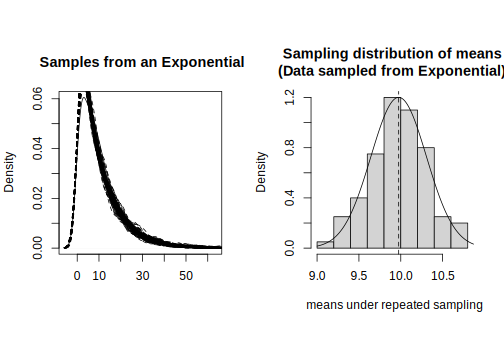
\includegraphics[width=0.75\linewidth]{Freq_CogSci_files/figure-latex/sdsmexp-1} \caption{Sampling from an exponential.}\label{fig:sdsmexp}
\end{figure}

A further example is samples from a Gamma distribution. Suppose we sample from a Gamma distribution with shape parameter chosen arbitrarily to be 1. The distribution of means is again going to be approximately normal.

\begin{figure}
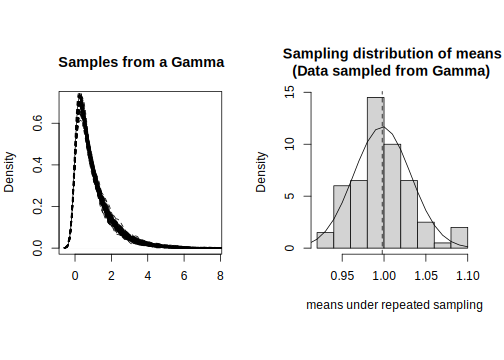
\includegraphics[width=0.75\linewidth]{Freq_CogSci_files/figure-latex/sdsmgamma-1} \caption{Sampling from a Gamma distribution.}\label{fig:sdsmgamma}
\end{figure}

As a final example, consider what happens if sample from a distribution, the Cauchy, that doesn't have any mean or variance defined for it.

\begin{figure}
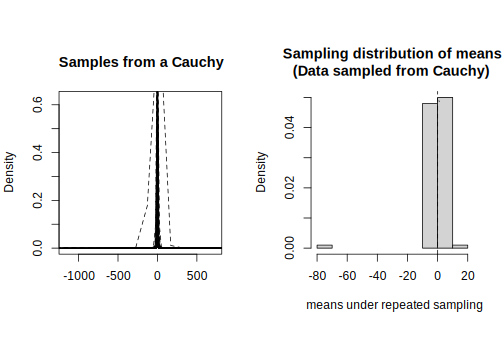
\includegraphics[width=0.75\linewidth]{Freq_CogSci_files/figure-latex/sdsmcauchy-1} \caption{Sampling from a Cauchy distribution.}\label{fig:sdsmcauchy}
\end{figure}

As the figure illustrates, when the mean and variance for the likelihood are undefined, the central limit theorem doesn't hold. In the rest of this book, we will always assume that the data are coming from a distribution that has a mean and variance defined for it.

\hypertarget{the-confidence-interval-and-what-its-good-for}{%
\section{The confidence interval, and what it's good for}\label{the-confidence-interval-and-what-its-good-for}}

Once we have sample of data \(y\), and once the sample mean \(\bar{y}\) and the \(SE = s/\sqrt{n}\) have been computed, it is common to define a so-called 95\% confidence interval:

\begin{equation}
\bar{y} \pm 2 SE
\end{equation}

Because the sampling distribution of means is normally distributed, and because 95\% of the area under the curve is covered by two times the standard deviation of the normal distribution,\\
the upper and lower bounds of the interval defined by the interval \(\bar{y} \pm 2 SE\) covers approximately 95\% of the area under the curve in the sampling distribution.

This interval is called the \emph{confidence interval} (CI) and has the following meaning: If you take samples repeatedly and compute the CI each time, 95\% of those CIs will contain the true population mean \(\mu\). One can simulate this situation. This time we will do 1000 repeated experiments instead of 100.

\begin{Shaded}
\begin{Highlighting}[]
\NormalTok{mu <-}\StringTok{ }\DecValTok{500}
\NormalTok{sigma <-}\StringTok{ }\DecValTok{100}
\NormalTok{n <-}\StringTok{ }\DecValTok{1000}
\NormalTok{nsim <-}\StringTok{ }\DecValTok{1000}
\NormalTok{lower <-}\StringTok{ }\KeywordTok{rep}\NormalTok{(}\OtherTok{NA}\NormalTok{, nsim)}
\NormalTok{upper <-}\StringTok{ }\KeywordTok{rep}\NormalTok{(}\OtherTok{NA}\NormalTok{, nsim)}
\ControlFlowTok{for}\NormalTok{ (i }\ControlFlowTok{in} \DecValTok{1}\OperatorTok{:}\NormalTok{nsim) \{}
\NormalTok{  y <-}\StringTok{ }\KeywordTok{rnorm}\NormalTok{(n, }\DataTypeTok{mean =}\NormalTok{ mu, }\DataTypeTok{sd =}\NormalTok{ sigma)}
\NormalTok{  lower[i] <-}\StringTok{ }\KeywordTok{mean}\NormalTok{(y) }\OperatorTok{-}\StringTok{ }\DecValTok{2} \OperatorTok{*}\StringTok{ }\KeywordTok{sd}\NormalTok{(y)}\OperatorTok{/}\KeywordTok{sqrt}\NormalTok{(n)}
\NormalTok{  upper[i] <-}\StringTok{ }\KeywordTok{mean}\NormalTok{(y) }\OperatorTok{+}\StringTok{ }\DecValTok{2} \OperatorTok{*}\StringTok{ }\KeywordTok{sd}\NormalTok{(y)}\OperatorTok{/}\KeywordTok{sqrt}\NormalTok{(n)}
\NormalTok{\}}

\CommentTok{## check how many CIs contain mu:}
\NormalTok{CIs <-}\StringTok{ }\KeywordTok{ifelse}\NormalTok{(lower }\OperatorTok{<}\StringTok{ }\NormalTok{mu }\OperatorTok{&}\StringTok{ }\NormalTok{upper }\OperatorTok{>}\StringTok{ }\NormalTok{mu, }\DecValTok{1}\NormalTok{, }\DecValTok{0}\NormalTok{)}
\CommentTok{## approx. 95% of the CIs contain true mean:}
\KeywordTok{round}\NormalTok{(}\KeywordTok{table}\NormalTok{(CIs)[}\DecValTok{2}\NormalTok{]}\OperatorTok{/}\KeywordTok{sum}\NormalTok{(}\KeywordTok{table}\NormalTok{(CIs)), }\DecValTok{2}\NormalTok{)}
\end{Highlighting}
\end{Shaded}

\begin{verbatim}
##    1 
## 0.94
\end{verbatim}

Figure \ref{fig:ciplot} visualizes the coverage properties of the confidence interval in 100 simulations; by coverage we mean here the proportion of cases where the true \(\mu\) is contained in the CI.

\textbackslash{}begin\{figure\}
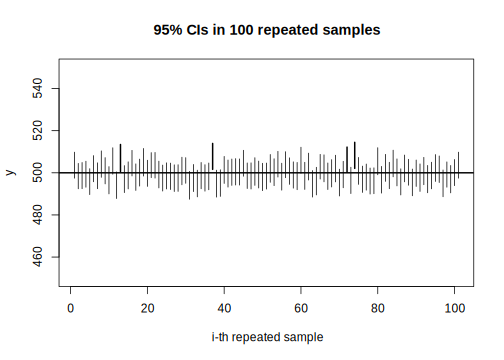
\includegraphics[width=0.75\linewidth]{Freq_CogSci_files/figure-latex/ciplot-1} \textbackslash{}caption\{Illustration of the meaning of the 95\% confidence interval. The dark bars are CIs which do not contain the true mean.\}\label{fig:ciplot}
\textbackslash{}end\{figure\}

The confidence interval is widely misinterpreted in a Bayesian way, i.e., as representing the range of plausible value of the \(\mu\) parameter. This is the wrong interpretation because \(\mu\) is a point value by assumption, it doesn't have a PDF associated with it. By contrast, the Bayesian credible interval does have this interpretation.
In practice, we find that in most modeling settings we have encountered, the frequentist and Bayesian credible interval have very similar widths, with the Bayesian interval being slightly wider depending on the prior specifications.

Given the convoluted meaning of the CI, and the impossibility of interpreting a single CI, it is reasonable to ask: what good is a CI? One can treat the CI as a graphical summary of width of the sampling distribution of the mean---the wider the sampling distribution, the more the implied variability under repeated sampling. The confidence interval can therefore be used as a visual summary of how uncertain we can be about the estimate of the sample mean under hypothetical repeated sampling. See \citet{cumming2014new} for a useful perspective relating to using confidence intervals for inference.

We turn next to the central ideas behind the hypothesis test. We begin with the humble one-sample t-test, which contains many subtleties and is well worth close study before we move on to the main topic of this book: linear mixed models.

\hypertarget{hypothesis-testing-the-one-sample-t-test}{%
\section{Hypothesis testing: The one sample t-test}\label{hypothesis-testing-the-one-sample-t-test}}

With the central limit theorem and the idea of hypothetical repeated sampling behind us, we turn now to one of the simplest statistical tests that one can do with continuous data: the t-test.

Due to its simplicity, it is tempting to take only a cursory look at the t-test and move on immediately to the linear (mixed) model. This would be a mistake. The humble t-test is surprising in many ways, and holds several important lessons for us. There are subtleties in this test, and a close connection to the linear mixed model. For these reasons, it is worth slowing down and spending some time understanding this test. Once the t-test is clear, more complex statistical tests will be easier to follow, because the logic of these more complex tests will essentially be more of the same, or variations on this general theme. You will see later that t-test can be seen as an analysis of variance or ANOVA; and the paired t-test is exactly the linear mixed model with varying intercepts.

\hypertarget{the-one-sample-t-test}{%
\subsection{The one-sample t-test}\label{the-one-sample-t-test}}

As in our running example, suppose we have a random sample \(y\) of size \(n\), and the data come from a \(N(\mu,\sigma)\) distribution, with unknown parameters \(\mu\) and \(\sigma\). We can estimate \(\mu\) from the sample mean \(\bar{y}\), which we will sometimes also write as \(\hat \mu\). We can also estimate \(\sigma\) from the sample standard deviation \(s\), which we can also write as \(\hat\sigma\). These estimates in turn allow us to estimate the sampling distribution of the mean under (hypothetical) repeated sampling:

\begin{equation}
N(\hat\mu,\frac{\hat \sigma}{\sqrt{n}})
\end{equation}

It is important to realize here that the above sampling distribution is only as realistic as the estimates of the mean and standard deviation parameters---if those are inaccurately estimated, then the sampling distribution is not realistic either.

Assume as before that we take an independent random sample of size \(1000\) from a random variable \(Y\) that is normally distributed, with mean 500 and standard deviation 100. As usual, begin by estimating the mean and SE:

\begin{Shaded}
\begin{Highlighting}[]
\NormalTok{n <-}\StringTok{ }\DecValTok{1000}
\NormalTok{mu <-}\StringTok{ }\DecValTok{500}
\NormalTok{sigma <-}\StringTok{ }\DecValTok{100}
\CommentTok{## generate simulated data:}
\NormalTok{y <-}\StringTok{ }\KeywordTok{rnorm}\NormalTok{(}\DecValTok{1000}\NormalTok{, }\DataTypeTok{mean =} \DecValTok{500}\NormalTok{, }\DataTypeTok{sd =} \DecValTok{100}\NormalTok{)}
\CommentTok{## compute summary statistics:}
\NormalTok{y_bar <-}\StringTok{ }\KeywordTok{mean}\NormalTok{(y)}
\NormalTok{SE <-}\StringTok{ }\KeywordTok{sd}\NormalTok{(y)}\OperatorTok{/}\KeywordTok{sqrt}\NormalTok{(n)}
\end{Highlighting}
\end{Shaded}

The null hypothesis significance testing (NHST) approach as practised in psychology and other areas is to set up a null hypothesis that \(\mu\) has some fixed value. Just as an example, assume that our null hypothesis is:

\begin{equation}
H_0: \mu = 450
\end{equation}

This amounts to assuming that the true sampling distribution of sample means is (approximately) normally distributed and centered around 450, with the standard error estimated from the data.

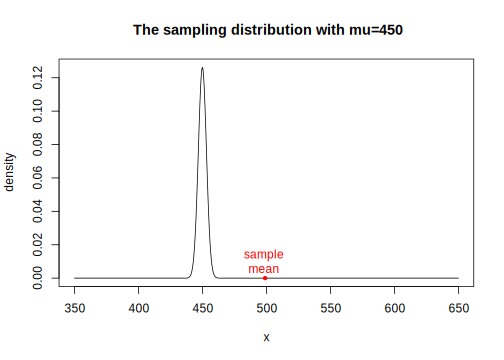
\includegraphics{Freq_CogSci_files/figure-latex/unnamed-chunk-35-1.pdf}

The intuitive idea here is that
- if the sample mean \(\bar{y}\) is ``near'' the hypothesized \(\mu\) (here, 450), the data are possibly consistent with the null hypothesis distribution.
- if the sample mean \(\bar{y}\) is ``far'' from the hypothesized \(\mu\), the data are inconsistent with the null hypothesis distribution.

The terms ``near'' and ``far'' will be quantified by determining how many standard error units the sample mean is from the hypothesized mean. This way of thinking shifts the focus away from the sampling distribution above, towards the distance measured in standard error units.

The distance between the sample mean and the hypothesized mean can be written in SE units. We will say that the sample mean is \(t\) standard errors away from the hypothesized mean:

\begin{equation}
t \times SE = \bar{x} - \mu 
\end{equation}

If we divide both sides with the standard error, we obtain the so-called observed t-statistic:

\begin{equation}
t  = \frac{\bar{x} - \mu}{SE}
\end{equation}

This observed t-value, an expression of the distance between the sample mean and the hypothesized mean, becomes the basis for the statistical test.

Notice that the t-value is a random variable: it is a transformation of \(\bar{X}\), the random variable generating the sample means. The t-value can therefore be seen as an instance of the following transformed random variable \(T\):

\begin{equation}
T  = \frac{\bar{X} - \mu}{SE}
\end{equation}

This random variable has a PDF associated with it, the t-distribution, which is defined in terms of the sample size \(n\); the pdf is written \(t(n-1)\). Under repeated sampling, the t-distribution is generated from this random variable \(T\).

We will compactly express the statement that ``the observed t-value is assumed to be generated under repeated sampling from a t-distribution with n-1 degrees of freedom'' as:

\begin{equation}
T \sim t(n-1)
\end{equation}

For large \(n\), the PDF of the random variable \(T\) approaches \(N(0,1)\). This is illustrated in Figure \ref{fig:tnormal}; notice that the t-distribution has fatter tails than the normal for small \(n\), say \(n<20\), but for larger n, the t-distribution and the normal are essentially identical. Incidentally, when n=2, the t-distribution \(t(1)\) is the Cauchy distribution we saw earlier; this distribution is characterized by fat tails, and has no mean or variance defined for it.

\begin{figure}
\centering
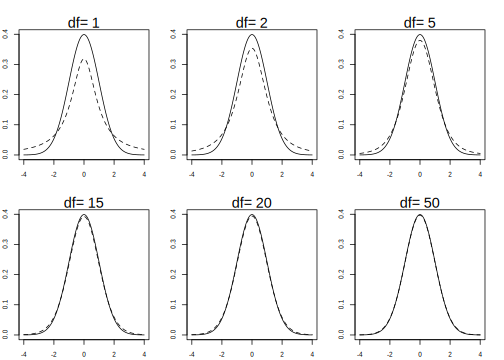
\includegraphics{Freq_CogSci_files/figure-latex/tnormal-1.pdf}
\caption{\label{fig:tnormal}A visual comparison of the t-distribution (with degrees of freedom ranging from 1 to 50) with the standard normal distribution (N(0,1)).}
\end{figure}

Thus, given a sample size \(n\), we can define a t-distribution corresponding to the null hypothesis distribution. For large values of \(n\), we could even use \(N(0,1)\), although it is traditional in psychology and linguistics to always use the t-distribution no matter how large \(n\) is.

The null hypothesis testing procedure proceeds as follows:

\begin{itemize}
\tightlist
\item
  Define the null hypothesis: in our example, the null hypothesis was that \(\mu = 450\). This amounts to making a commitment about what fixed value we think the true underlying distribution of sample means is centered at.
\item
  Given data of size \(n\), estimate \(\bar{y}\), standard deviation \(s\), and from that, estimate the standard error \(s/\sqrt{n}\). The standard error will be used to describe the sampling distribution's standard deviation.
\item
  Compute the observed t-value:
\end{itemize}

\begin{equation}
t=\frac{\bar{y}-\mu}{s/\sqrt{n}}
\end{equation}

\begin{itemize}
\tightlist
\item
  Reject null hypothesis if the observed t-value is ``large'' (to be made more precise next).
\item
  Fail to reject the null hypothesis, or (under some conditions) even go so far as to accept the null hypothesis, if the observed t-value is ``small''.
\end{itemize}

What constitutes a large or small observed t-value?
Intuitively, the t-value from the sample is large when we end up far in \emph{either} tail of the distribution. The two tails of the t-distribution will be referred to as the \emph{rejection region}. The word \emph{region} here refers to the real number line along the x-axis, under the tails of the distribution. The rejection region will go off to infinity on the outer sides, and is demarcated by a vertical line on the inner side of each tail. This is shown in Figure \ref{fig:tails}. It goes off to infinity because the support---the range of possible values---of the random variable that the t-distribution belongs to stretches from minus infinity to plus infinity.

\begin{figure}
\centering
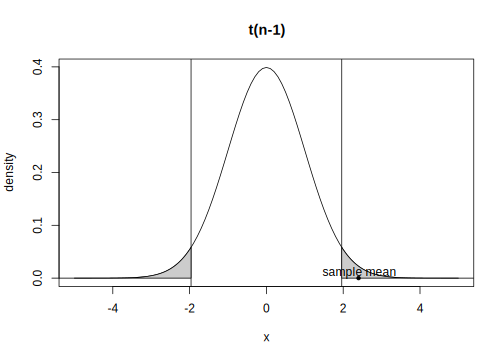
\includegraphics{Freq_CogSci_files/figure-latex/tails-1.pdf}
\caption{\label{fig:tails}The rejection region in a t-distribution.}
\end{figure}

The location of the vertical lines is determined by the so-called \emph{critical t-value} along the x-axis of the t-distribution. This is the value such that the area under the curve in the tails to the left or right of the tails is 0.025. As discussed in chapter 1, this area under the curve represents the probability of observing a value as extreme as the critical t-value, or some value that is more extreme. Notice that if we ask ourselves what the probability is of observing some particular t-value (a point value), the answer must necessarily be \(0\) (if you are unclear about why, re-read chapter 1). But we can ask the question: what is the absolute t-value, written \(|t|\), such that \(P(T>|t|)=0.025\)? That's the critical t-value.

For a given sample size \(n\), we can identify the rejection region by using the \texttt{qt} function, whose usage is analogous to the \texttt{qnorm} function, discussed in chapter 1.

Because the shape of the t-distribution depends on the degrees of freedom (n-1), the critical t-value beyond which we reject the null hypothesis will change depending on sample size. For large sample sizes, say \(n>50\), the rejection point is about 2.

\begin{Shaded}
\begin{Highlighting}[]
\KeywordTok{abs}\NormalTok{(}\KeywordTok{qt}\NormalTok{(}\FloatTok{0.025}\NormalTok{, }\DataTypeTok{df =} \DecValTok{15}\NormalTok{))}
\end{Highlighting}
\end{Shaded}

\begin{verbatim}
## [1] 2.131
\end{verbatim}

\begin{Shaded}
\begin{Highlighting}[]
\KeywordTok{abs}\NormalTok{(}\KeywordTok{qt}\NormalTok{(}\FloatTok{0.025}\NormalTok{, }\DataTypeTok{df =} \DecValTok{50}\NormalTok{))}
\end{Highlighting}
\end{Shaded}

\begin{verbatim}
## [1] 2.009
\end{verbatim}

Consider the observed t-value from our sample in our running example:

\begin{Shaded}
\begin{Highlighting}[]
\CommentTok{## null hypothesis mean:}
\NormalTok{mu <-}\StringTok{ }\DecValTok{450}
\NormalTok{(t_value <-}\StringTok{ }\NormalTok{(y_bar }\OperatorTok{-}\StringTok{ }\NormalTok{mu)}\OperatorTok{/}\NormalTok{SE)}
\end{Highlighting}
\end{Shaded}

\begin{verbatim}
## [1] 15.49
\end{verbatim}

This observed t-value is huge and is telling you the distance of the sample mean from the null hypothesis mean \(\mu\) in standard error units.

\begin{equation}
t=\frac{\bar{y}-\mu_0}{s/\sqrt{n}} \hbox{ or } t\frac{s}{\sqrt{n}}=\bar{y}-\mu_0
\end{equation}

For large sample sizes, if the absolute t-value \(|t|\) is greater than \(2\) (approximately), we will reject the null hypothesis. The choice of \(2\) is purely conventional and comes from standard practice in psychology and related disciplines (as we will see in this book, standard practice is sometimes not a good-enough reason to decide on such things!).

For a smaller sample size \(n\), you can compute the exact critical t-value:

\begin{Shaded}
\begin{Highlighting}[]
\KeywordTok{qt}\NormalTok{(}\FloatTok{0.025}\NormalTok{, }\DataTypeTok{df =}\NormalTok{ n }\OperatorTok{-}\StringTok{ }\DecValTok{1}\NormalTok{)}
\end{Highlighting}
\end{Shaded}

\begin{verbatim}
## [1] -1.962
\end{verbatim}

Why is this critical t-value negative in sign? That is because it is on the left-hand side of the t-distribution, which is symmetric.
The corresponding value on the right-hand side is:

\begin{Shaded}
\begin{Highlighting}[]
\KeywordTok{qt}\NormalTok{(}\FloatTok{0.975}\NormalTok{, }\DataTypeTok{df =}\NormalTok{ n }\OperatorTok{-}\StringTok{ }\DecValTok{1}\NormalTok{)}
\end{Highlighting}
\end{Shaded}

\begin{verbatim}
## [1] 1.962
\end{verbatim}

These values are of course identical if we ignore the sign. This is why we always frame our discussion around the absolute t-value.

In R, the built-in function \texttt{t.test} delivers the observed t-value. Given our running example, with the null hypothesis \(\mu=450\), R returns the following:

\begin{Shaded}
\begin{Highlighting}[]
\CommentTok{## observed t-value from t-test function:}
\KeywordTok{t.test}\NormalTok{(y, }\DataTypeTok{mu =} \DecValTok{450}\NormalTok{)}\OperatorTok{$}\NormalTok{statistic}
\end{Highlighting}
\end{Shaded}

\begin{verbatim}
##     t 
## 15.49
\end{verbatim}

The default value for the null hypothesis mean \(\mu\) in this function is 0; so if one doesn't define a null hypothesis mean, the statistical test is done with reference to a null hypothesis that \(\mu=0\). That is why this t-value does not match our calculation above:

\begin{Shaded}
\begin{Highlighting}[]
\KeywordTok{t.test}\NormalTok{(y)}\OperatorTok{$}\NormalTok{statistic}
\end{Highlighting}
\end{Shaded}

\begin{verbatim}
##     t 
## 157.8
\end{verbatim}

In the most common usage of the t-test, the null hypothesis mean will be \(0\), because usually one is comparing a difference in means between two conditions or two sets of conditions. So the above line of code will work out correctly in those cases; but if you ever have a different null hypothesis mean than \(0\), then you have to specify it in the \texttt{t.test} function.

So, the t-test is used as if it furnishes a \emph{decision rule}: either reject the null hypothesis or fail to reject it. Whenever we do an experiment and carry out a t-test, we use the t-test to make a decision: reject or fail to reject the null hypothesis.

Recall that behind the t-test lies the assumption that the observed t-value is coming from a random variable, \(T\sim t(n-1)\). The particular t-value we observe from a particular data-set belongs to a distribution of t-values under hypothetical repeated sampling. Thus, implicit in the logic of the t-test---and indeed every frequentist statistical test---is the assumption that the experiment is in principle repeatable: the experiment can in principle be re-run as many times as we want, assuming we have the necessary resources and time.

This implicit idea of the experiment's repeatability leads to an important aspect of the t-test: its long-run properties. In other words, its ability (at least in theory) to lead the researchers to the correct decision in the long run, i.e., under (hypothetical) repeated sampling. We turn to this issue next.

\hypertarget{type-i-ii-error-and-power}{%
\subsection{Type I, II error, and power}\label{type-i-ii-error-and-power}}

When we do a hypothesis test using the t-test, the observed t-value will either fall in the rejection region, leading us to reject the null hypothesis,
or it will land in the non-rejection region, leading us to fail to reject the null. That is a single, one-time event.

However, the null hypothesis can be either true or not true; we don't know which of those two possibilities is the reality.
When we say that the null could be true, we mean that the parameter \(\mu\) actually does have the hypothesized value \(\mu_0\); when we say that the null could be false, we mean that the parameter \(\mu\) has some \emph{specific} value \(\mu_{alt}\) other than \(\mu_0\).
We can represent these two alternative possible realities in a tabular form, as shown below. The two columns show the two possible worlds, one in which the null is true, and the other in which it is false. The two rows show the two possible decisions we can take based on the observed t-value: reject the null or fail to reject it.

\begin{tabular}{ccc}
        & \textbf{Possible world 1}      & \textbf{Possible world 2} \\  
\hline
 & $H_0$ TRUE: $\mu=\mu_0$  & $H_0$ FALSE $\mu=\mu_{alt}$ \\
\hline
Decision: `reject': & $\alpha$ & $1~-~\beta$ \\
                                     & Type I error                         & Power \\                                      
                                     & & \\
\hline
Decision: `fail to reject': & $1 - \alpha$ & $\beta$ \\                                    &                                 & Type II error\\
\hline
\end{tabular}

As the table shows, we can make two kinds of mistakes:

\begin{itemize}
\tightlist
\item
  Type I error or \(\alpha\): Reject the null when it's true.
\item
  Type II error or \(\beta\): Accept the null when it's false.
\end{itemize}

In psychology and related areas, Type I error is fixed a priori at 0.05. This stipulated Type I error value is why the absolute critical t-value is kept at approximately \(2\); if, following recommendations from \citet{benjamin2018redefine}, we were to stipulate that the Type I error be 0.005, then the critical t-value would have had to be set at:

\begin{Shaded}
\begin{Highlighting}[]
\KeywordTok{abs}\NormalTok{(}\KeywordTok{qt}\NormalTok{(}\FloatTok{0.0025}\NormalTok{, }\DataTypeTok{df =}\NormalTok{ n }\OperatorTok{-}\StringTok{ }\DecValTok{1}\NormalTok{))}
\end{Highlighting}
\end{Shaded}

\begin{verbatim}
## [1] 2.813
\end{verbatim}

This suggested change in convention hasn't been taken up yet in cognitive science, but this could well change one day.

Type II error, the probability of incorrectly accepting the null hypothesis when it is false with some particular value for the parameter \(\mu\), is conventionally recommended (e.g., by the American Psychological Association) to be kept at 0.20 or lower. This implies that the probability of correctly rejecting a null hypothesis for some particular true value of \(\mu\) is 1-Type II error. This probability, called statistical power, or just power, should then obviously be larger than 0.80. Again, there is nothing special about these stipulations; they are conventions that became the norm over time.

Next, we will consider the trade-off between Type I and II error. For simplicity, assume that the standard error is 1, and the null hypothesis is that \(\mu=0\). This means that the t-value is really the sample mean.

Consider the concrete situation where, in reality, the true value of \(\mu\) is \(2\). As mentioned above, the null hypothesis \(H_0\) is that \(\mu=0\). Now the \(H_0\) is false because \(\mu=2\) and not \(0\). Type I and II error can be visualized graphically as shown in Figure \ref{fig:type12}.

\begin{figure}
\centering
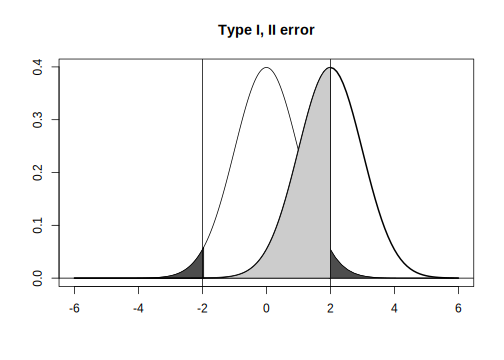
\includegraphics{Freq_CogSci_files/figure-latex/type12-1.pdf}
\caption{\label{fig:type12}A visualization of Type I and II error. The dark-shaded tails of the left-hand side distribution represent Type I error; and the light-colored shaded region of the right-hand side distribution represents Type II error. Power is the unshaded area under the curve in the right-hand side distribution.}
\end{figure}

To understand Figure \ref{fig:type12}, one has to consider two distributions side by side. First, consider the null hypothesis distribution, centered at 0. Under the null hypothesis distribution, the rejection region lies below the dark colored tails of the distributions. The area under the curve in these dark-colored tails is the Type I error (conventionally set at 0.05) that we decide on before we even conduct the experiment and collect the data. Because the Type I error is set at 0.05, and because the t-distribution is symmetric, the area under the curve in each tail is 0.025. The absolute critical t-value helps us demarcates the inner boundaries of the rejection regions through the vertical lines shown in the figure. These vertical lines play a crucial role in helping us understand Type II error and power. This becomes clear when we consider the distribution representing the alternative possible value of \(\mu\), the distribution centered around 2. In this second distribution, consider now the area under the curve between the vertical lines demarcating the rejection region under the null. This area under the curve is the probability of accepting the null hypothesis when the null hypothesis is false with some specific value (here, when \(\mu\) has value 2).

Some interesting observations follow. Suppose that the true effect is in fact \(\mu=2\), as in the above illustration. Then,

\begin{itemize}
\tightlist
\item
  Simply decreasing Type I error to a smaller value like 0.005 will also increase Type II error, which means that power (1-Type II error) will fall.
\item
  Increasing sample size will squeeze the vertical lines closer to each other, reducing Type II error, and therefore increasing power. Decreasing sample size will have the opposite effect.
\item
  If we design an experiment with a larger effect size, e.g., by setting up a stronger manipulation (concete examples will be discussed in this book later on), our Type II error will go down, and therefore power will go up. Figure \ref{fig:highpower} shows a graphical visualization of a situation where the true effect size is \(\mu=4\). Here, Type II error is much smaller compared to Figure \ref{fig:type12}, where \(\mu=2\).
\end{itemize}

\begin{figure}
\centering
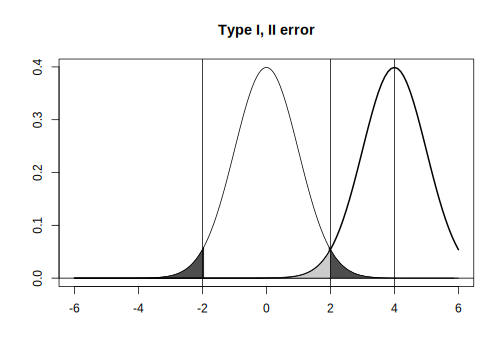
\includegraphics{Freq_CogSci_files/figure-latex/highpower-1.pdf}
\caption{\label{fig:highpower}The change in Type II error if the true effect has mean 4.}
\end{figure}

In summary, when we plan out an experiment, we are also required to specify the Type I and II error associated with the design. Both sources of error are within our control, at least to some extent. The Type I error we decide to use will determine our critical t-value and therefore our decision criterion for rejecting, failing to reject, or even (under certain conditions, to be discussed below) accepting the null hypothesis.

The Type II error we decide on will determine the long-run probability of incorrectly accepting the null hypothesis; its inverse (1-Type II error), statistical power, will determine the long-run probability of correctly rejecting the null hypothesis under the assumption that the \(\mu\) has some particular assumed value.

That's the theory anyway. In practice, researchers only rarely consider the power properties of their experiment design; the focus is almost exclusively on Type I error. The neglect of power in experiment design has had interesting consequences for theory development, as we will see later in this book. For a case study in psycholinguistics, see \citet{VasishthMertzenJaegerGelman2018}.

\hypertarget{how-to-compute-power-for-the-one-sample-t-test}{%
\subsection{How to compute power for the one-sample t-test}\label{how-to-compute-power-for-the-one-sample-t-test}}

Power is a function of three variables:

\begin{itemize}
\tightlist
\item
  the effect size
\item
  the standard deviation
\item
  the sample size.
\end{itemize}

There are two ways that one can compute power in connection with the t-test: either one can use the built-in R function, \texttt{power.t.test}, or one can use simulation.

\hypertarget{power-calculation-using-the-power.t.test}{%
\subsubsection{Power calculation using the power.t.test}\label{power-calculation-using-the-power.t.test}}

Suppose that we have an expectation that an effect size is 15 ms \(\pm 5\) ms (this could be based on the predictions of a theoretical model, or prior data); suppose also that prior experiments show standard deviations ranging from 100 to 300 ms. This is enough information to compute a power curve as a function of effect size and standard deviation. See Figure \ref{fig:powercurve} and the associated code below.

\begin{Shaded}
\begin{Highlighting}[]
\NormalTok{sds <-}\StringTok{ }\KeywordTok{seq}\NormalTok{(}\DecValTok{100}\NormalTok{, }\DecValTok{300}\NormalTok{, }\DataTypeTok{by =} \DecValTok{1}\NormalTok{)}
\NormalTok{lower <-}\StringTok{ }\KeywordTok{power.t.test}\NormalTok{(}\DataTypeTok{delta =} \DecValTok{15} \OperatorTok{-}\StringTok{ }\DecValTok{5}\NormalTok{, }\DataTypeTok{sd =}\NormalTok{ sds, }\DataTypeTok{n =} \DecValTok{10}\NormalTok{, }
  \DataTypeTok{strict =} \OtherTok{TRUE}\NormalTok{)}\OperatorTok{$}\NormalTok{power}
\NormalTok{upper <-}\StringTok{ }\KeywordTok{power.t.test}\NormalTok{(}\DataTypeTok{delta =} \DecValTok{15} \OperatorTok{+}\StringTok{ }\DecValTok{5}\NormalTok{, }\DataTypeTok{sd =}\NormalTok{ sds, }\DataTypeTok{n =} \DecValTok{10}\NormalTok{, }
  \DataTypeTok{strict =} \OtherTok{TRUE}\NormalTok{)}\OperatorTok{$}\NormalTok{power}
\NormalTok{meanval <-}\StringTok{ }\KeywordTok{power.t.test}\NormalTok{(}\DataTypeTok{delta =} \DecValTok{15}\NormalTok{, }\DataTypeTok{sd =}\NormalTok{ sds, }\DataTypeTok{n =} \DecValTok{10}\NormalTok{, }
  \DataTypeTok{strict =} \OtherTok{TRUE}\NormalTok{)}\OperatorTok{$}\NormalTok{power}

\KeywordTok{plot}\NormalTok{(sds, meanval, }\DataTypeTok{type =} \StringTok{"l"}\NormalTok{, }\DataTypeTok{main =} \StringTok{"Power curve (n=10)}\CharTok{\textbackslash{}n}\StringTok{ using power.t.test"}\NormalTok{, }
  \DataTypeTok{xlab =} \StringTok{"standard deviation"}\NormalTok{, }\DataTypeTok{ylab =} \StringTok{"effect size"}\NormalTok{)}
\KeywordTok{lines}\NormalTok{(sds, lower, }\DataTypeTok{lty =} \DecValTok{2}\NormalTok{)}
\KeywordTok{lines}\NormalTok{(sds, upper, }\DataTypeTok{lty =} \DecValTok{2}\NormalTok{)}
\KeywordTok{text}\NormalTok{(}\DecValTok{200}\NormalTok{, }\FloatTok{0.05}\NormalTok{, }\StringTok{"10"}\NormalTok{)}
\KeywordTok{text}\NormalTok{(}\DecValTok{200}\NormalTok{, }\FloatTok{0.054}\NormalTok{, }\StringTok{"15"}\NormalTok{)}
\KeywordTok{text}\NormalTok{(}\DecValTok{200}\NormalTok{, }\FloatTok{0.056}\NormalTok{, }\StringTok{"20"}\NormalTok{)}
\end{Highlighting}
\end{Shaded}

\begin{figure}
\centering
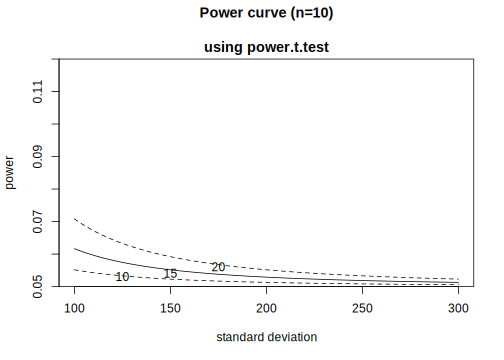
\includegraphics{Freq_CogSci_files/figure-latex/powercurve-1.pdf}
\caption{\label{fig:powercurve}An illustration of a power curve for 10 participants, as a function of standard deviation, and three estimates of the effect: 15, 10, and 20.}
\end{figure}

\hypertarget{power-calculations-using-simulation}{%
\subsubsection{Power calculations using simulation}\label{power-calculations-using-simulation}}

An analogous calculation as the one shown above using the \texttt{power.t.test} function can also be done using simulated data.
First, generate simulated data repeatedly for each possible combination of parameter values (here, effect size and standard deviation), and compute the proportion of significant effects for each parameter combination. This can be done by defining a function that takes as input the number of simulations, sample size, effect size, and standard deviation:

\begin{Shaded}
\begin{Highlighting}[]
\NormalTok{compute_power <-}\StringTok{ }\ControlFlowTok{function}\NormalTok{(}\DataTypeTok{nsim =} \DecValTok{1000}\NormalTok{, }\DataTypeTok{n =} \DecValTok{10}\NormalTok{, }\DataTypeTok{effect =} \OtherTok{NULL}\NormalTok{, }
  \DataTypeTok{stddev =} \OtherTok{NULL}\NormalTok{) \{}
\NormalTok{  temp_power <-}\StringTok{ }\KeywordTok{rep}\NormalTok{(}\OtherTok{NA}\NormalTok{, nsim)}
  \ControlFlowTok{for}\NormalTok{ (i }\ControlFlowTok{in} \DecValTok{1}\OperatorTok{:}\NormalTok{nsim) \{}
\NormalTok{    y <-}\StringTok{ }\KeywordTok{rnorm}\NormalTok{(n, }\DataTypeTok{mean =}\NormalTok{ effect, }\DataTypeTok{sd =}\NormalTok{ stddev)}
\NormalTok{    temp_power[i] <-}\StringTok{ }\KeywordTok{ifelse}\NormalTok{(}\KeywordTok{abs}\NormalTok{(}\KeywordTok{t.test}\NormalTok{(y)}\OperatorTok{$}\NormalTok{statistic) }\OperatorTok{>}\StringTok{ }
\StringTok{      }\DecValTok{2}\NormalTok{, }\DecValTok{1}\NormalTok{, }\DecValTok{0}\NormalTok{)}
\NormalTok{  \}}
  \CommentTok{## return power calculation:}
  \KeywordTok{mean}\NormalTok{(temp_power)}
\NormalTok{\}}
\end{Highlighting}
\end{Shaded}

Then, plot the power curves as a function of effect size and standard deviation, exactly as in Figure \ref{fig:powercurve}. Power calculations using simulations are shown in Figure \ref{fig:powercurve2}. It is clear that simulation-based power estimation is going to be noisy; this is because each time we are generating simulated data and then carrying out a statistical test on it. This is no longer a closed-form mathematical calculation as done in \texttt{power.t.test} (this function simply implements a formula for power calculation specified for this simple case). Because the power estimates will be noisy, we show a smoothed lowess line for each effect size estimate.

\begin{figure}
\centering
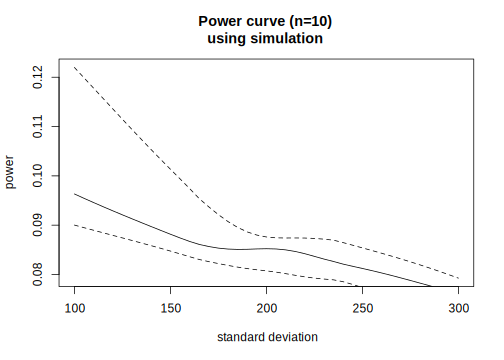
\includegraphics{Freq_CogSci_files/figure-latex/powercurve2-1.pdf}
\caption{\label{fig:powercurve2}An illustration of a power curve using simulation, for 10 participants, as a function of standard deviation, and three estimates of the effect: 15, 10, and 20. The power curves are lowess-smoothed.}
\end{figure}

In the above example, simulation-based power calculation is overkill, and completely unnecessary because we have \texttt{power.t.test}. However, the technique shown above will be extended and will become our bread-and-butter method once we switch to power calculations for complicated linear mixed models. There, no closed form calculation can be done to compute power, at least not without oversimplifying the model; simulation will be the only practical way to calculate power.

It is important to appreciate the fact that power is a \emph{function}; it isn't a single number. Because we can never be sure what the true effect size is, or what the true standard deviation is, we should always aim to report a power function, as a function of plausible values of the relevant parameters.

\hypertarget{the-p-value}{%
\subsection{The p-value}\label{the-p-value}}

Continuing with our t-test example, the \texttt{t.test} function in R will not only print out a t-value as shown above, but also a probability known as a \emph{p-value}. This is the probability of obtaining the observed t-value that we did, or some value more extreme than that, conditional on the assumption that the null hypothesis is true.

We can compute the p-value ``by hand''. This can be computed, as done earlier, simply by calculating the area under the curve that lies beyond the observed t-value. It is standard practice to take the tail probability on both sides of the t-distribution.

\begin{Shaded}
\begin{Highlighting}[]
\NormalTok{(t_value <-}\StringTok{ }\KeywordTok{t.test}\NormalTok{(y, }\DataTypeTok{mu =} \DecValTok{450}\NormalTok{)}\OperatorTok{$}\NormalTok{statistic)}
\end{Highlighting}
\end{Shaded}

\begin{verbatim}
##     t 
## 15.49
\end{verbatim}

\begin{Shaded}
\begin{Highlighting}[]
\DecValTok{2} \OperatorTok{*}\StringTok{ }\KeywordTok{pt}\NormalTok{(}\KeywordTok{abs}\NormalTok{(t_value), }\DataTypeTok{df =}\NormalTok{ n }\OperatorTok{-}\StringTok{ }\DecValTok{1}\NormalTok{, }\DataTypeTok{lower.tail =} \OtherTok{FALSE}\NormalTok{)}
\end{Highlighting}
\end{Shaded}

\begin{verbatim}
##         t 
## 8.529e-08
\end{verbatim}

The area from both sides of the tail is taken because it is conventional to do a so-called \emph{two-sided t-test}: our null hypothesis is that \(\mu=450\), and our alternative hypothesis is two-sided: \(\mu\) is either less than 450 or \(\mu\) is larger than 450. When we reject the null hypothesis, we are accepting this alternative, that \(\mu\) could be some value other than 450. Notice that this alternative hypothesis is remarkably vague; we would reject the null hypothesis regardless of whether the sample mean turns out to be 600 or -600, for example. The practical implication is that the p-value gives us the strength of the evidence against the null hypothesis; it doesn't give us evidence in favor of a specific alternative, such as saying that \(\mu\) is positive or negative in sign. In psychology and allied disciplines, whenever the p-value falls below \(0.05\), it is common practice to write something along the lines that ``there was reliable evidence for the predicted effect.'' This statement is technically incorrect; we only ever have evidence against the null. By looking at the sample mean and its sign, we are making a very big leap that we have evidence for the specific sample mean we happened to get. As we will see below, the sample mean can be wildly far from the true mean that produced the data.

One need not have done a two-sided alternative; one could have defined the alternative to be one-sided. In that case, one would compute only one side of the area under the curve. This kind of one-sided test is not normally done, but one can imagine a situation where a one-sided test is justified (for example, when only one sign of the effect is possible, or if there is a strong theoretical reason to expect only one particular sign---positive or negative---on an effect). That said, in their scientific career, none of the authors of this book have ever had occasion to use a one-sided test.

The p-value is always interpreted with reference to the pre-defined Type I error. Conventionally, we reject the null if \(p<0.05\). This is because we set the Type I error at 0.05. Keep in mind that Type I error and the p-value are two distinct things.
Type I error is the probability of your incorrectly rejecting the null under repeated sampling. This is not the same thing as your p-value. The latter will be obtained from a particular experiment, and will vary from experiment to experiment; it is a random variable. Type I error is a value we fix in advance.

\hypertarget{the-distribution-of-the-p-value-under-the-null-hypothesis}{%
\subsubsection{*The distribution of the p-value under the null hypothesis}\label{the-distribution-of-the-p-value-under-the-null-hypothesis}}

We have been talking about a continuous random variable as a dependent measure, and have learnt about the standard two-sided t-test, with a point null hypothesis. When we do such a test, we usually use the p-value to decide whether to reject the null hypothesis or not.

Sometimes, you will hear statisticians (e.g., Andrew Gelman on his blog) say that the null hypothesis significance test is a specific random number generator. What does that sentence mean? We explain this point here.

It's worth briefly reflecting on the fact that the p-value is a random variable; call it \(Z\). The p-value is the cumulative distribution function (CDF) of the random variable \(T\), which itself is a transformation of the random variable \(\bar{Y}\):

\(T=(\bar{X}-\mu)/(\sigma/\sqrt{n})\)

This random variable \(T\) has some CDF \(F(T)\). It is possible to show that if a random variable \(Z=F(T)\), i.e., if \(Z\) is the
CDF for the random variable \(T\), then \(Z \sim Uniform(0,1)\).

This is an amazing fact. To get a grip on this, let's first think about the fact that when a random variable \(Z\) comes from a \(Uniform(0,1)\) distribution, then \(P(Z<z)=z\). Consider some examples:

\begin{itemize}
\tightlist
\item
  when \(z=0\), then \(P(Z<0)=0\);
\item
  when \(z=0.25\), then \(P(Z<0.25)=0.25\);
\item
  when \(z=0.5\), then \(P(Z<0.5)=0.5\);
\item
  when \(z=0.75\), then \(P(Z<0.75)=0.75\);
\item
  when \(z=1\), then \(P(Z<1)=1\).
\end{itemize}

Next, we will prove the above statement, that if a random variable \(Z=F(T)\), i.e., if \(Z\) is the
CDF for a random variable \(T\), then \(Z \sim Uniform(0,1)\).
The proof is actually quite astonishing and even has a name: it's called the \emph{probability integral transform}.

Suppose that \(Z\) is the CDF of a random variable \(T\): \(Z=F(T)\). Then, it follows that \(P(Z\leq z)\) can be rewritten in terms of the CDF of T: \(P(F(T)\leq z)\). Now, if we apply the inverse of the CDF (\(F^{-1}\)) to both the left and right sides of the inequality, we get \(P(F^{-1}F(T)\leq F^{-1}(z))\).
But \(F^{-1}F(T)\) gives us back \(T\); this holds because if we have a one-to-one onto function \(f(x)\), then applying the inverse \(f^{-1}\) to this function gives us back \(x\).

The fact that \(F^{-1}F(T)\) gives us back \(T\) means that we can rewrite \(P(F^{-1}F(T)\leq F^{-1}(z))\) as \(P(T\leq F^{-1}(z) )\). But this probability is simply the CDF \(F(F^{-1} (z))\), which simplifies to \(z\). This shows that \(P(Z\leq z) = z\); i.e., that the p-value has a uniform distribution under the null hypothesis.

The above proof is restated below compactly:

\begin{equation}
\begin{split}
P(Z\leq z) =& P(F(T)\leq z)\\
=& P(F^{-1}F(T)\leq F^{-1}(z))\\
=& P(T\leq F^{-1}(z) ) \\
=& F(F^{-1} (z))\\
=& z\\
\end{split}
\end{equation}

It is for this reason that statisticians like Andrew Gelman periodically point out that ``the null hypothesis significance test is a specific random number generator''. The practical implication of this observation is that we should not place our theory development exclusively at the feet of the p-value. As we discuss in this book, other considerations (such as replicability, uncertainty of the estimates, and power) are as or even more important.

\hypertarget{type-m-and-s-error-in-the-face-of-low-power}{%
\subsection{Type M and S error in the face of low power}\label{type-m-and-s-error-in-the-face-of-low-power}}

Beyond Type I and II error, there are also two other kinds of error to be aware of. These are Type M and S error; both sources of error are closely related to statistical power.

The terms Type M and S error were introduced by \citet{Gelman14}, but the ideas has been in existence for some time \citep[\citet{lane1978estimating}]{hedges1984estimation}. \citet{powerfailure} refer to Type M and S error as the ``winner's curse'' and ``the vibration of effects.'' In related work, \citet{ioannidis2008most} discusses refers to the vibration ratio in the context of epidemiology.

Type S and M error can be illustrated with the following example.
Suppose your true effect size is believed to be \(D=15\),
then we can compute (apart from statistical power) the following error rates, which are defined as follows:

\begin{itemize}
\tightlist
\item
  \textbf{Type S error}: the probability that the sign of the effect is incorrect, given that the result is statistically significant.
\item
  \textbf{Type M error}: the expectation of the ratio of the absolute magnitude of the effect to the hypothesized true effect size, given that result is significant.
  Gelman and Carlin also call this the exaggeration ratio, which is perhaps more descriptive than ``Type M error''.
\end{itemize}

Suppose that our particular study has standard error \(46\), and sample size \(37\). And suppose that our true \(\mu=15\), as stated above. Then, we can compute statistical power, Type S and M error through simulation in the following manner:

\begin{Shaded}
\begin{Highlighting}[]
\CommentTok{## probable effect size, derived from past studies:}
\NormalTok{D <-}\StringTok{ }\DecValTok{15}
\CommentTok{## SE from the study of interest:}
\NormalTok{se <-}\StringTok{ }\DecValTok{46}
\NormalTok{stddev <-}\StringTok{ }\NormalTok{se }\OperatorTok{*}\StringTok{ }\KeywordTok{sqrt}\NormalTok{(}\DecValTok{37}\NormalTok{)}
\NormalTok{nsim <-}\StringTok{ }\DecValTok{10000}
\NormalTok{drep <-}\StringTok{ }\KeywordTok{rep}\NormalTok{(}\OtherTok{NA}\NormalTok{, nsim)}
\ControlFlowTok{for}\NormalTok{ (i }\ControlFlowTok{in} \DecValTok{1}\OperatorTok{:}\NormalTok{nsim) \{}
\NormalTok{  samp <-}\StringTok{ }\KeywordTok{rnorm}\NormalTok{(}\DecValTok{37}\NormalTok{, }\DataTypeTok{mean =}\NormalTok{ D, }\DataTypeTok{sd =}\NormalTok{ stddev)}
\NormalTok{  drep[i] <-}\StringTok{ }\KeywordTok{mean}\NormalTok{(samp)}
\NormalTok{\}}
\end{Highlighting}
\end{Shaded}

Power can be computed by simply determining the proportion of times that the absolute observed t-value is larger than 2:

\begin{Shaded}
\begin{Highlighting}[]
\CommentTok{## power: the proportion of cases where we reject}
\CommentTok{## the null hypothesis correctly:}
\NormalTok{(pow <-}\StringTok{ }\KeywordTok{mean}\NormalTok{(}\KeywordTok{ifelse}\NormalTok{(}\KeywordTok{abs}\NormalTok{(drep}\OperatorTok{/}\NormalTok{se) }\OperatorTok{>}\StringTok{ }\DecValTok{2}\NormalTok{, }\DecValTok{1}\NormalTok{, }\DecValTok{0}\NormalTok{)))}
\end{Highlighting}
\end{Shaded}

\begin{verbatim}
## [1] 0.0608
\end{verbatim}

Power is quite low here (we deliberately chose an example with low power to illustrate Type S and M error).

Next, we figure out which of the cases are statistically significant (which simulated values yield \(p<0.05\)). As a criterion, we use a t-value of 2 to declare \(p<0.05\); we could have done this more precisely by working out an exact critical t-value.

\begin{Shaded}
\begin{Highlighting}[]
\CommentTok{## which results in drep are significant at}
\CommentTok{## alpha=0.05?}
\NormalTok{signif <-}\StringTok{ }\KeywordTok{which}\NormalTok{(}\KeywordTok{abs}\NormalTok{(drep}\OperatorTok{/}\NormalTok{se) }\OperatorTok{>}\StringTok{ }\DecValTok{2}\NormalTok{)}
\end{Highlighting}
\end{Shaded}

Type S error is the proportion of significant cases with the wrong sign (sign error), and Type M error is the ratio by the true effect (of \(\mu=15\)) is exaggerated in those simulations that happened to come out significant.

\begin{Shaded}
\begin{Highlighting}[]
\CommentTok{## Type S error rate | signif:}
\NormalTok{(types_sig <-}\StringTok{ }\KeywordTok{mean}\NormalTok{(drep[signif] }\OperatorTok{<}\StringTok{ }\DecValTok{0}\NormalTok{))}
\end{Highlighting}
\end{Shaded}

\begin{verbatim}
## [1] 0.1645
\end{verbatim}

\begin{Shaded}
\begin{Highlighting}[]
\CommentTok{## Type M error rate | signif:}
\NormalTok{(typem_sig <-}\StringTok{ }\KeywordTok{mean}\NormalTok{(}\KeywordTok{abs}\NormalTok{(drep[signif])}\OperatorTok{/}\NormalTok{D))}
\end{Highlighting}
\end{Shaded}

\begin{verbatim}
## [1] 7.414
\end{verbatim}

In this scenario, when power is approximately 6\%, whenever we get a significant effect, the probability of obtaining the wrong sign is a whopping 16\% and the effect is likely to be 7.4144 times larger than its true magnitude. The practical implication is as follows.

When power is low, relying on the p-value (statistical significance) to declare an effect as being present will be misleading because the decision will be based on an overestimate of the effect (Type M error), and even the sign of the effect could be wrong. This isn't just a theoretical point; it has real-world consequences for theory development. For an example from psycholinguistics regarding this point, see \citet{VasishthMertzenJaegerGelman2018}.

Another useful way to visualize Type M and S error is through the so-called funnel plot. As shown in Figure \ref{fig:funnel}, estimates obtained from low-powered studies will tend to be exaggerated (the lower part of the funnel), and as power goes up, the effect estimates start to cluster tightly around the true value of the effect.

\begin{figure}
\centering
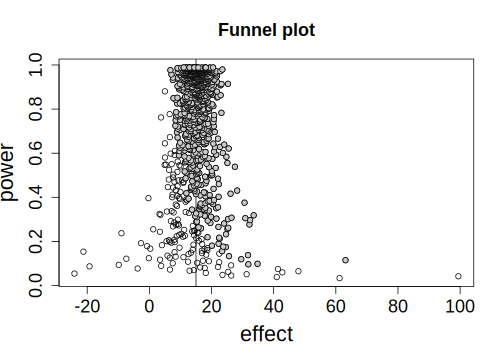
\includegraphics{Freq_CogSci_files/figure-latex/funnel-1.pdf}
\caption{\label{fig:funnel}An illustration of a funnel plot. Shown are repeated samples of an effect estimate under different values of power, where the true value of the effect is 15 (marked by the vertical line). Significant effects are shaded gray. The lower the power, the wider the fluctuation of the effect; under low power, it is the exaggerated effects that end up statistically significant, even though they are very biased relative to the true value. As power goes up, the effect estimates start to cluster around the true value, and significant effects are also accurate estimates of the effect. Thus, low power leads to exaggerated estimates of the effect, especially if the data are filtered by statistical significance.}
\end{figure}

What is important to appreciate here is the fact that significant effects ``point to the truth'' just in case power is high; when power is low, either null results will frequently be found even if the null is false, and those results that turn out significant will be based on Type M error.

In many fields, it is practically impossible to conduct a high-powered study. What should one do in this situation? When reporting results that are likely based on an underpowered study, the best approach ia to openly acknowledge the power limitation, to attempt to conduct a direct replication of the effect to establish robustness, and to attempt to synthesize the evidence from existing knowlege \citep{cumming2014new}.

By direct replication, we mean that the study should be run multiple times with the same materials and design but new participants, to establish whether effect estimates in the original study and the replication study are consistent with each other. Direct replications stand in contrast to so-called conceptual replications, which are not exact repetitions of the original design, but involve some further or slightly different but related experimental manipulation. Conceptual replications are also a very useful tool for cross-validating the existence of an effect.

Direct replications will always differ from the original study in some way or another---the lab may differ, the protocols might differ slightly, the experimenter is different, etc. Such between-study variability is obviously unavoidable in direct-replication attempts, but they are still worthwhile for establishing the existence of an effect. To make the idea of establishing robustness through replication attempts, detailed examples of different kinds of replication attempts will be presented in this book's example data-sets.

\hypertarget{searching-for-significance}{%
\subsection{Searching for significance}\label{searching-for-significance}}

The NHST procedure is essentially a decision procedure: if \(p<0.05\), we reject the null hypothesis; otherwise, we fail to reject the null. Because significant results are easier to publish than non-significant results, a common approach taken by researchers (including the first author of this book, when he was a graduate student) is to run the experiment and periodically check if statistical significance has been reached. The procedure can be described as follows:

\begin{itemize}
\tightlist
\item
  The experimenter gathers \(n\) data points, then checks for significance (is \(p<0.05\) or not?).
\item
  If the result is not significant, he gets more data (say, \(n\) more data points). Then he checks for significance, and repeats.
\end{itemize}

Since time and money are limited, he might decide to stop collecting data after some multiple of \(n\) have been collected.

One can simulate different scenarios here. Suppose that \(n\) is initially \(15\).\\
Under the standard assumptions, we set Type I error to be \(0.05\). Let's suppose that the null hypothesis that \(\mu=0\) is in fact true, and that standard deviation is 250.

\begin{Shaded}
\begin{Highlighting}[]
\CommentTok{## Standard properties of the t-test:}
\NormalTok{pvals <-}\StringTok{ }\OtherTok{NULL}
\NormalTok{tstat_standard <-}\StringTok{ }\OtherTok{NULL}
\NormalTok{n <-}\StringTok{ }\DecValTok{15}
\NormalTok{nsim <-}\StringTok{ }\DecValTok{10000}
\CommentTok{## assume a standard dev of 1:}
\NormalTok{stddev <-}\StringTok{ }\DecValTok{250}
\NormalTok{mn <-}\StringTok{ }\DecValTok{0}
\ControlFlowTok{for}\NormalTok{ (i }\ControlFlowTok{in} \DecValTok{1}\OperatorTok{:}\NormalTok{nsim) \{}
\NormalTok{  samp <-}\StringTok{ }\KeywordTok{rnorm}\NormalTok{(n, }\DataTypeTok{mean =}\NormalTok{ mn, }\DataTypeTok{sd =}\NormalTok{ stddev)}
\NormalTok{  pvals[i] <-}\StringTok{ }\KeywordTok{t.test}\NormalTok{(samp)}\OperatorTok{$}\NormalTok{p.value}
\NormalTok{  tstat_standard[i] <-}\StringTok{ }\KeywordTok{t.test}\NormalTok{(samp)}\OperatorTok{$}\NormalTok{statistic}
\NormalTok{\}}
\end{Highlighting}
\end{Shaded}

Type I error rate is about 5\%, consistent with our expectations:

\begin{Shaded}
\begin{Highlighting}[]
\KeywordTok{round}\NormalTok{(}\KeywordTok{table}\NormalTok{(pvals }\OperatorTok{<}\StringTok{ }\FloatTok{0.05}\NormalTok{)[}\DecValTok{2}\NormalTok{]}\OperatorTok{/}\NormalTok{nsim, }\DecValTok{2}\NormalTok{)}
\end{Highlighting}
\end{Shaded}

\begin{verbatim}
## TRUE 
## 0.05
\end{verbatim}

But the situation quickly deteriorates as soon as we adopt the strategy outlined above. Below, we will also track the distribution of the t-statistic.

\begin{Shaded}
\begin{Highlighting}[]
\NormalTok{pvals <-}\StringTok{ }\OtherTok{NULL}
\NormalTok{tstat <-}\StringTok{ }\OtherTok{NULL}
\CommentTok{## how many subjects can I run?}
\NormalTok{upper_bound <-}\StringTok{ }\NormalTok{n }\OperatorTok{*}\StringTok{ }\DecValTok{6}

\ControlFlowTok{for}\NormalTok{ (i }\ControlFlowTok{in} \DecValTok{1}\OperatorTok{:}\NormalTok{nsim) \{}
\NormalTok{  significant <-}\StringTok{ }\OtherTok{FALSE}
\NormalTok{  x <-}\StringTok{ }\KeywordTok{rnorm}\NormalTok{(n, }\DataTypeTok{mean =}\NormalTok{ mn, }\DataTypeTok{sd =}\NormalTok{ stddev)  }\CommentTok{## take sample}
  \ControlFlowTok{while}\NormalTok{ (}\OperatorTok{!}\NormalTok{significant }\OperatorTok{&}\StringTok{ }\KeywordTok{length}\NormalTok{(x) }\OperatorTok{<}\StringTok{ }\NormalTok{upper_bound) \{}
    \CommentTok{## if not significant:}
    \ControlFlowTok{if}\NormalTok{ (}\KeywordTok{t.test}\NormalTok{(x)}\OperatorTok{$}\NormalTok{p.value }\OperatorTok{>}\StringTok{ }\FloatTok{0.05}\NormalTok{) \{}
\NormalTok{      x <-}\StringTok{ }\KeywordTok{append}\NormalTok{(x, }\KeywordTok{rnorm}\NormalTok{(n, }\DataTypeTok{mean =}\NormalTok{ mn, }\DataTypeTok{sd =}\NormalTok{ stddev))  }\CommentTok{## get more data}
\NormalTok{    \} }\ControlFlowTok{else}\NormalTok{ \{}
\NormalTok{      significant <-}\StringTok{ }\OtherTok{TRUE}
\NormalTok{    \}  }\CommentTok{## otherwise stop:}
\NormalTok{  \}}
\NormalTok{  pvals[i] <-}\StringTok{ }\KeywordTok{t.test}\NormalTok{(x)}\OperatorTok{$}\NormalTok{p.value}
\NormalTok{  tstat[i] <-}\StringTok{ }\KeywordTok{t.test}\NormalTok{(x)}\OperatorTok{$}\NormalTok{statistic}
\NormalTok{\}}
\end{Highlighting}
\end{Shaded}

Now, Type I error rate is much higher than 5\%:

\begin{Shaded}
\begin{Highlighting}[]
\KeywordTok{round}\NormalTok{(}\KeywordTok{table}\NormalTok{(pvals }\OperatorTok{<}\StringTok{ }\FloatTok{0.05}\NormalTok{)[}\DecValTok{2}\NormalTok{]}\OperatorTok{/}\NormalTok{nsim, }\DecValTok{2}\NormalTok{)}
\end{Highlighting}
\end{Shaded}

\begin{verbatim}
## TRUE 
## 0.15
\end{verbatim}

Figure \ref{fig:stoppingrule} shows the distributions of the t-statistic in the standard case vs with the above stopping rule:

\begin{figure}
\centering
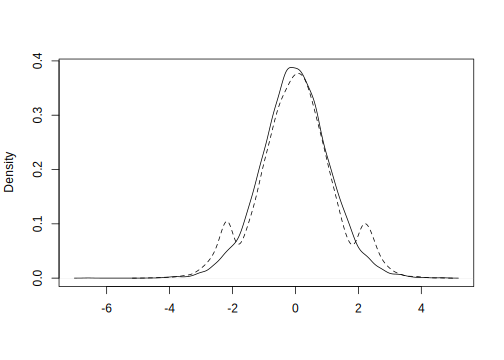
\includegraphics{Freq_CogSci_files/figure-latex/stoppingrule-1.pdf}
\caption{\label{fig:stoppingrule}A comparison of the distribution of t-values with an a priori fixed stopping rule, versus a flexible stopping rule conditional on finding significance.}
\end{figure}

What is important to realize here is that the inflation in Type I error we observed above was due to the fact that the t-distribution is no longer a t-distribution: we have bumps in the tails when we use the flexible stopping rule, and these raise our Type I error. This demonstrates why one should fix one's sample size in advance, based on a power analysis. One should not deploy a stopping rule like the one above; if we used such a stopping rule, we are much more likely to incorrectly declare a result as statistically significant. There can be compelling reasons to adopt the peek-and-run strategy; e.g., if one wants to avoid exposing patients to a treatment that might turn out to be harmful. In such situations, one can run an adaptive experimental trial by correcting for Type I error inflation \citep{pocock2013clinical}. In this book, we will aim to develop a workflow whereby the sample size is fixed through power analysis, in advance of running an experiment.

\hypertarget{the-two-sample-t-test-vs.the-paired-t-test}{%
\section{The two-sample t-test vs.~the paired t-test}\label{the-two-sample-t-test-vs.the-paired-t-test}}

In our running example above, we examined the case where we have a single vector of data \(y\). This led to the one-sample t-test.

Next, we consider a case where we have two vectors of data. The data-set below is from \citet{johnson2011quantitative}. Shown below are F1 formant data (in Herz), productions of different vowels by male and female speakers of different languages.

\begin{Shaded}
\begin{Highlighting}[]
\NormalTok{F1data <-}\StringTok{ }\KeywordTok{read.table}\NormalTok{(}\StringTok{"data/F1_data.txt"}\NormalTok{, }\DataTypeTok{header =} \OtherTok{TRUE}\NormalTok{)}
\NormalTok{F1data}
\end{Highlighting}
\end{Shaded}

\begin{verbatim}
##    female male vowel  language
## 1     391  339     i  W.Apache
## 2     561  512     e  W.Apache
## 3     826  670     a  W.Apache
## 4     453  427     o  W.Apache
## 5     358  291     i CAEnglish
## 6     454  406     e CAEnglish
## 7     991  706     a CAEnglish
## 8     561  439     o CAEnglish
## 9     398  324     u CAEnglish
## 10    334  307     i   Ndumbea
## 11    444  361     e   Ndumbea
## 12    796  678     a   Ndumbea
## 13    542  474     o   Ndumbea
## 14    333  311     u   Ndumbea
## 15    343  293     i      Sele
## 16    520  363     e      Sele
## 17    989  809     a      Sele
## 18    507  367     o      Sele
## 19    357  300     u      Sele
\end{verbatim}

Notice that the male and female values can be seen as \emph{dependent} or \emph{paired}: each row belongs to the same vowel and language. Nevertheless, we can compare males' and females' F1 frequencies, completely ignoring this paired nature of the data. The t-test does not ``know'' whether these data are paired or not---it is the researcher's job to make sure that model assumptions are met.

Let's ignore the paired nature of the data for now, and treat the two vectors as independent vectors. Suppose that our null hypothesis is that there is no difference between the mean F1's for males (\(\mu_m\)) and females (\(\mu_f\)).
Now, our null hypothesis is \(H_0: \mu_m = \mu_f\) or \(H_0: \mu_m - \mu_f = \delta = 0\).

This kind of statistical test calls for a two-sample t-test. Note here that we are assuming that both the male and female F1 scores have equal variance.

The function call in R for a two-sample t-test is shown below:

\begin{Shaded}
\begin{Highlighting}[]
\KeywordTok{t.test}\NormalTok{(F1data}\OperatorTok{$}\NormalTok{female, F1data}\OperatorTok{$}\NormalTok{male, }\DataTypeTok{paired =} \OtherTok{FALSE}\NormalTok{, }
  \DataTypeTok{var.equal =} \OtherTok{TRUE}\NormalTok{)}
\end{Highlighting}
\end{Shaded}

\begin{verbatim}
## 
## 	Two Sample t-test
## 
## data:  F1data$female and F1data$male
## t = 1.5, df = 36, p-value = 0.1
## alternative hypothesis: true difference in means is not equal to 0
## 95 percent confidence interval:
##  -30.07 217.54
## sample estimates:
## mean of x mean of y 
##     534.6     440.9
\end{verbatim}

This t-test is computing the following t-statistic:

\begin{equation}
t=\frac{d-(\mu_m - \mu_f)}{SE} = \frac{d-0}{SE} 
\end{equation}

\noindent 
where \(d\) is the difference between the two sample means; the rest of the terms we are familiar with. SE is the standard error of the sampling distribution of the difference between the means.

We will now do this calculation ``by hand''. The only new things are the formula for the SE calculation, and the degrees of freedom for t-distribution \((2\times n - 2)=36\).

The standard error for the difference in the means in the two-sample t-test is computed using this formula:

\begin{equation}
SE_\delta 
= \sqrt{\frac{\hat\sigma_m^2}{n_m} + \frac{\hat\sigma_f^2}{n_f}}
\end{equation}

Here, \(\hat\sigma_m\) is estimate of the standard deviation for males, and \(\hat\sigma_f\) for the females; the \(n\) are the respective sample sizes.

\begin{Shaded}
\begin{Highlighting}[]
\NormalTok{n_m <-}\StringTok{ }\NormalTok{n_f <-}\StringTok{ }\DecValTok{19}
\CommentTok{## difference of sample means:}
\NormalTok{d <-}\StringTok{ }\KeywordTok{mean}\NormalTok{(F1data}\OperatorTok{$}\NormalTok{female) }\OperatorTok{-}\StringTok{ }\KeywordTok{mean}\NormalTok{(F1data}\OperatorTok{$}\NormalTok{male)}
\NormalTok{(SE <-}\StringTok{ }\KeywordTok{sqrt}\NormalTok{(}\KeywordTok{var}\NormalTok{(F1data}\OperatorTok{$}\NormalTok{male)}\OperatorTok{/}\NormalTok{n_m }\OperatorTok{+}\StringTok{ }\KeywordTok{var}\NormalTok{(F1data}\OperatorTok{$}\NormalTok{female)}\OperatorTok{/}\NormalTok{n_f))}
\end{Highlighting}
\end{Shaded}

\begin{verbatim}
## [1] 61.04
\end{verbatim}

\begin{Shaded}
\begin{Highlighting}[]
\NormalTok{(observed_t <-}\StringTok{ }\NormalTok{(d }\OperatorTok{-}\StringTok{ }\DecValTok{0}\NormalTok{)}\OperatorTok{/}\NormalTok{SE)}
\end{Highlighting}
\end{Shaded}

\begin{verbatim}
## [1] 1.536
\end{verbatim}

\begin{Shaded}
\begin{Highlighting}[]
\CommentTok{## p-value:}
\DecValTok{2} \OperatorTok{*}\StringTok{ }\NormalTok{(}\DecValTok{1} \OperatorTok{-}\StringTok{ }\KeywordTok{pt}\NormalTok{(observed_t, }\DataTypeTok{df =} \DecValTok{36}\NormalTok{))}
\end{Highlighting}
\end{Shaded}

\begin{verbatim}
## [1] 0.1334
\end{verbatim}

The output of the two-sample t-test and the hand-calculation above match up.

Now consider what will change once we take into account the fact that the data are paired. The two-sample t-test now becomes a so-called paired t-test.

For such paired data, the null hypothesis is as before: \(H_0: \delta=0\). But since each row in the data-frame is paired (from the same vowel+language), we subtract the vector row-wise, and get a new \emph{vector} \(d\) (not a single number \(d\) as in the two-sample t-test) with the row-wise differences. Then, we just do the familiar one-sample test we saw earlier:

\begin{Shaded}
\begin{Highlighting}[]
\NormalTok{d <-}\StringTok{ }\NormalTok{F1data}\OperatorTok{$}\NormalTok{female }\OperatorTok{-}\StringTok{ }\NormalTok{F1data}\OperatorTok{$}\NormalTok{male}
\KeywordTok{t.test}\NormalTok{(d)}
\end{Highlighting}
\end{Shaded}

\begin{verbatim}
## 
## 	One Sample t-test
## 
## data:  d
## t = 6.1, df = 18, p-value = 9e-06
## alternative hypothesis: true mean is not equal to 0
## 95 percent confidence interval:
##   61.48 125.99
## sample estimates:
## mean of x 
##     93.74
\end{verbatim}

An alternative syntax for the paired t-test explicitly feeds the two paired vectors into the function, but one must explicitly specify that they are paired, otherwise the test is a two-sample (i.e., unpaired) t-test:

\begin{Shaded}
\begin{Highlighting}[]
\KeywordTok{t.test}\NormalTok{(F1data}\OperatorTok{$}\NormalTok{female, F1data}\OperatorTok{$}\NormalTok{male, }\DataTypeTok{paired =} \OtherTok{TRUE}\NormalTok{)}
\end{Highlighting}
\end{Shaded}

\begin{verbatim}
## 
## 	Paired t-test
## 
## data:  F1data$female and F1data$male
## t = 6.1, df = 18, p-value = 9e-06
## alternative hypothesis: true difference in means is not equal to 0
## 95 percent confidence interval:
##   61.48 125.99
## sample estimates:
## mean of the differences 
##                   93.74
\end{verbatim}

Incidentally, notice that the p-value in the paired t-test is statistically significant, unlike the two-sample t-test above. The null hypothesis is the same in both tests, but the significance level leads to different conclusions.

Which analysis is correct, the two-sample t-test or the paired t-test? It all depends on your assumptions about what the data represent. If you consider the data paired, for the reasons given above, then a paired test is called for. If the pairing (the same vowel and language in each row) is unlikely to create a dependency between the two data points in a row (here, domain knowledge is required), we can treat this as unpaired data.

Next, we look at some perhaps subtle points about the paired t-test.

\hypertarget{common-mistakes-involving-the-t-test}{%
\subsection{Common mistakes involving the t-test}\label{common-mistakes-involving-the-t-test}}

The paired t-test assumes that each row in the data-frame is independent of the other rows. This implies that the data-frame cannot have more than one row for a particular pair. In other words, the data-frame cannot have repeated measurements spread out across rows.

For example, doing a paired t-test on this hypothetical data-frame would be incorrect:

\begin{table}[ht]
\centering
\begin{tabular}{rrrll}
\hline
female & male & vowel & language \\ 
\hline
391 & 339 & i & W.Apache \\ 
400 & 320 & i & W.Apache \\ 
$\vdots$ & $\vdots$ & $\vdots$ & $\vdots$\\
\hline
\end{tabular}
\end{table}

Why? Because the assumption is that each row is independent of the others. This assumption is violated here (this is assuming that repeating the vowel from the same language will lead to some commonalities between the two repetitions).

Consider another hypothetical example. In the table below, from subject 1 we see two data points each for condition a and for condition b.

\begin{table}[ht]
\centering
\begin{tabular}{rrrll}
\hline
condition a & condition b & subject & item \\ 
\hline
391 & 339 & 1 & 1 \\ 
400 & 320 & 1 & 2 \\ 
$\vdots$ & $\vdots$ & $\vdots$ & $\vdots$\\
\hline
\end{tabular}
\end{table}

Here, we again have repeated measurements from subject 1. The independence assumption is violated.

How to proceed when we have repeated measurements from each subject or each item?
The solution is to aggregate the data so that each subject (or item) has only \emph{one} value for each condition.

This aggregation allows us to meet the independence assumption of the t-test, but it has a potentially huge drawback: it pretends we have one measurement from each subject for each condition.
Later on we will learn how to analyze unaggregated data, but if we want to do a paired t-test, we have no choice but to aggregate the data in this way.

A fully worked example will make this clear. We have repeated measures data on subject versus object relative clauses in English. The data are from a self-paced reading study reported in \citet{grodner}, their experiment 1. A theoretical prediction is that in English, object relatives are harder to read than subject relatives, in the relative clause verb region. We want to test this prediction.

First, load the data containing reading times from the region of interest (the relative clause verb):

\begin{Shaded}
\begin{Highlighting}[]
\NormalTok{gg05e1 <-}\StringTok{ }\KeywordTok{read.table}\NormalTok{(}\StringTok{"data/grodnergibsonE1crit.txt"}\NormalTok{,}
                     
                     \DataTypeTok{header=}\OtherTok{TRUE}\NormalTok{)}

\KeywordTok{head}\NormalTok{(gg05e1)}
\end{Highlighting}
\end{Shaded}

\begin{verbatim}
##    subject item condition rawRT
## 6        1    1    objgap   320
## 19       1    2   subjgap   424
## 34       1    3    objgap   309
## 49       1    4   subjgap   274
## 68       1    5    objgap   333
## 80       1    6   subjgap   266
\end{verbatim}

We have repeated measurements for each condition from the subjects, and from items. You can establish this by using the \texttt{xtabs} command.
Notice that there are no missing data points:

\begin{Shaded}
\begin{Highlighting}[]
\KeywordTok{t}\NormalTok{(}\KeywordTok{xtabs}\NormalTok{(}\OperatorTok{~}\NormalTok{subject }\OperatorTok{+}\StringTok{ }\NormalTok{condition, gg05e1))}
\end{Highlighting}
\end{Shaded}

\begin{verbatim}
##          subject
## condition 1 2 3 4 5 6 7 8 9 10 11 12 13 14 15 16 17 18
##   objgap  8 8 8 8 8 8 8 8 8  8  8  8  8  8  8  8  8  8
##   subjgap 8 8 8 8 8 8 8 8 8  8  8  8  8  8  8  8  8  8
##          subject
## condition 19 20 21 22 23 24 25 26 27 28 29 30 31 32 33
##   objgap   8  8  8  8  8  8  8  8  8  8  8  8  8  8  8
##   subjgap  8  8  8  8  8  8  8  8  8  8  8  8  8  8  8
##          subject
## condition 34 35 36 37 38 39 40 41 42
##   objgap   8  8  8  8  8  8  8  8  8
##   subjgap  8  8  8  8  8  8  8  8  8
\end{verbatim}

\begin{Shaded}
\begin{Highlighting}[]
\KeywordTok{t}\NormalTok{(}\KeywordTok{xtabs}\NormalTok{(}\OperatorTok{~}\NormalTok{item }\OperatorTok{+}\StringTok{ }\NormalTok{condition, gg05e1))}
\end{Highlighting}
\end{Shaded}

\begin{verbatim}
##          item
## condition  1  2  3  4  5  6  7  8  9 10 11 12 13 14 15
##   objgap  21 21 21 21 21 21 21 21 21 21 21 21 21 21 21
##   subjgap 21 21 21 21 21 21 21 21 21 21 21 21 21 21 21
##          item
## condition 16
##   objgap  21
##   subjgap 21
\end{verbatim}

It is important to stress once more that it is the researcher's responsibility to make sure that the t-test's assumptions are met. For example, one could fit a two-sample t-test to the data as provided. The two-sample t-test can be implemented using the syntax shown below:

\begin{Shaded}
\begin{Highlighting}[]
\KeywordTok{t.test}\NormalTok{(rawRT }\OperatorTok{~}\StringTok{ }\NormalTok{condition, gg05e1)}
\end{Highlighting}
\end{Shaded}

\begin{verbatim}
## 
## 	Welch Two Sample t-test
## 
## data:  rawRT by condition
## t = 3.8, df = 431, p-value = 2e-04
## alternative hypothesis: true difference in means is not equal to 0
## 95 percent confidence interval:
##   48.98 155.59
## sample estimates:
##  mean in group objgap mean in group subjgap 
##                 471.4                 369.1
\end{verbatim}

This t-test is incorrect for several reasons, but the most egregious error here is that the data are paired (each subject delivers data for both conditions), and that property of the data is being ignored.

Another common mistake is to do a paired t-test on the data as provided. Again, the t.test function will happily return a meaningless result:

\begin{Shaded}
\begin{Highlighting}[]
\KeywordTok{t.test}\NormalTok{(rawRT }\OperatorTok{~}\StringTok{ }\NormalTok{condition, }\DataTypeTok{paired =} \OtherTok{TRUE}\NormalTok{, gg05e1)}
\end{Highlighting}
\end{Shaded}

\begin{verbatim}
## 
## 	Paired t-test
## 
## data:  rawRT by condition
## t = 4, df = 335, p-value = 8e-05
## alternative hypothesis: true difference in means is not equal to 0
## 95 percent confidence interval:
##   51.98 152.59
## sample estimates:
## mean of the differences 
##                   102.3
\end{verbatim}

Here, the degrees of freedom indicate that we have fit the incorrect model. There are 42 subjects and 16 items, and the presentation of items to subjects uses a Latin square design (each subject sees only one condition per item). The 335 degrees of freedom come from \(42\times 8=336\) data points, minus one. Why do we say \(42\times 8\) and not \(42\times 16\)? That is because each subject will return eight differences in reading time for each condition: each subject gives us eight subject-relative data points and eight object-relative data points.

For each of the 42 subjects, the t-test function internally creates a vector of eight data points of subject relatives and subtracts the vector of eight data points of object relatives. That is how we end up with \(42\times 8=336\) data points.

These 336 data points are assumed by the t-test to be independent of each other; but this cannot be the case because each subject delivers eight data points for each condition; these are obviously dependent (correlated) because they come from the same subject.

What is needed is a \emph{single} data-point for each subject and condition, and for each item and condition. In order to conduct the t-test, aggregation of the data by subjects and by items is necessary.

Consider the by-subjects aggregation procedure below. Now we have only one data-point for each condition and subject:

\begin{Shaded}
\begin{Highlighting}[]
\NormalTok{bysubj <-}\StringTok{ }\KeywordTok{aggregate}\NormalTok{(rawRT }\OperatorTok{~}\StringTok{ }\NormalTok{subject }\OperatorTok{+}\StringTok{ }\NormalTok{condition, mean, }
  \DataTypeTok{data =}\NormalTok{ gg05e1)}
\KeywordTok{t}\NormalTok{(}\KeywordTok{xtabs}\NormalTok{(}\OperatorTok{~}\NormalTok{subject }\OperatorTok{+}\StringTok{ }\NormalTok{condition, bysubj))}
\end{Highlighting}
\end{Shaded}

\begin{verbatim}
##          subject
## condition 1 2 3 4 5 6 7 8 9 10 11 12 13 14 15 16 17 18
##   objgap  1 1 1 1 1 1 1 1 1  1  1  1  1  1  1  1  1  1
##   subjgap 1 1 1 1 1 1 1 1 1  1  1  1  1  1  1  1  1  1
##          subject
## condition 19 20 21 22 23 24 25 26 27 28 29 30 31 32 33
##   objgap   1  1  1  1  1  1  1  1  1  1  1  1  1  1  1
##   subjgap  1  1  1  1  1  1  1  1  1  1  1  1  1  1  1
##          subject
## condition 34 35 36 37 38 39 40 41 42
##   objgap   1  1  1  1  1  1  1  1  1
##   subjgap  1  1  1  1  1  1  1  1  1
\end{verbatim}

Notice that the data are correlated: the longer the subject relative clause data from a participant, the longer their object relative clause data:

\begin{Shaded}
\begin{Highlighting}[]
\NormalTok{SRdata <-}\StringTok{ }\KeywordTok{subset}\NormalTok{(bysubj, condition }\OperatorTok{==}\StringTok{ "subjgap"}\NormalTok{)}\OperatorTok{$}\NormalTok{rawRT}
\NormalTok{ORdata <-}\StringTok{ }\KeywordTok{subset}\NormalTok{(bysubj, condition }\OperatorTok{==}\StringTok{ "objgap"}\NormalTok{)}\OperatorTok{$}\NormalTok{rawRT}
\KeywordTok{plot}\NormalTok{(SRdata, ORdata)}
\KeywordTok{abline}\NormalTok{(}\KeywordTok{lm}\NormalTok{(ORdata }\OperatorTok{~}\StringTok{ }\NormalTok{SRdata))}
\end{Highlighting}
\end{Shaded}

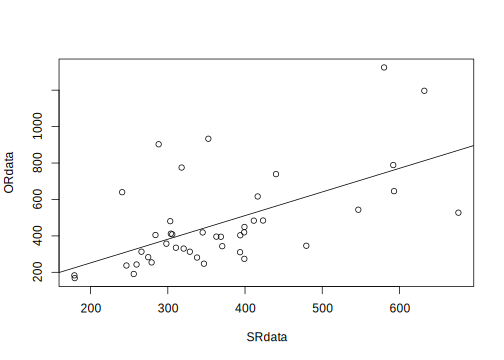
\includegraphics{Freq_CogSci_files/figure-latex/unnamed-chunk-63-1.pdf}

\begin{Shaded}
\begin{Highlighting}[]
\KeywordTok{cor}\NormalTok{(SRdata, ORdata)}
\end{Highlighting}
\end{Shaded}

\begin{verbatim}
## [1] 0.5876
\end{verbatim}

Returning to the t-test, by aggregating the data the t-test's assumptions are met, and the degrees of freedom for this by-subjects analysis are now correct (\(42-1=41\)):

\begin{Shaded}
\begin{Highlighting}[]
\KeywordTok{t.test}\NormalTok{(rawRT }\OperatorTok{~}\StringTok{ }\NormalTok{condition, bysubj, }\DataTypeTok{paired =} \OtherTok{TRUE}\NormalTok{)}
\end{Highlighting}
\end{Shaded}

\begin{verbatim}
## 
## 	Paired t-test
## 
## data:  rawRT by condition
## t = 3.1, df = 41, p-value = 0.003
## alternative hypothesis: true difference in means is not equal to 0
## 95 percent confidence interval:
##   35.85 168.72
## sample estimates:
## mean of the differences 
##                   102.3
\end{verbatim}

Similar to the by-subjects aggregation done above, one could do a by-items aggregation and then a by-items t-test (What should be the degrees of freedom for the by-items analysis? There are 16 items in this data-set). This is left as an exercise for the reader.

The paired t-test illustrated above is actually not the best way to analyze this data-set, because it ignores the fact that each subject delivers not one but eight data points per condition. Each subject's repeated measurements will introduce a source of variance, but this source of variance is being suppressed in this t-test, leading to a possibly over-enthusiastic t-value. In order to take this variability into account, we must switch to the linear mixed model. But before we get to the linear mixed model, we have to consider the linear model. The next chapter turns to this topic.

\hypertarget{sec:SamplingDistrnexercises}{%
\section{Exercises}\label{sec:SamplingDistrnexercises}}

\hypertarget{sec:SamplingDistrnexercisesPart1}{%
\subsection{Computing the p-value}\label{sec:SamplingDistrnexercisesPart1}}

A paired t-test is done with data from 10 participants. The t-value from the test is 2.1. What is the p-value associated with a two-sided null hypothesis test?

\hypertarget{sec:SamplingDistrnexercisesPart2}{%
\subsection{Computing the t-value}\label{sec:SamplingDistrnexercisesPart2}}

If the p-value from a two-sided null hypothesis test had been 0.09, what would be the associated absolute t-value (i.e., ignoring the sign on the t-value)? The number of participants is 10, as above.

\hypertarget{sec:SamplingDistrnexercisesPart3}{%
\subsection{Type I and II error}\label{sec:SamplingDistrnexercisesPart3}}

Given that Type I error is 0.01; what is the highest value possible for Type II error?

\hypertarget{linear-models-and-linear-mixed-models}{%
\chapter{Linear models and linear mixed models}\label{linear-models-and-linear-mixed-models}}

\hypertarget{from-the-t-test-to-the-linear-mixed-model}{%
\section{From the t-test to the linear (mixed) model}\label{from-the-t-test-to-the-linear-mixed-model}}

We begin with the \citet{grodner} self-paced reading data we saw in the previous chapter. Load the data and compute the means by condition at the relative clause verb:

\begin{Shaded}
\begin{Highlighting}[]
\NormalTok{gg05e1 <-}\StringTok{ }\KeywordTok{read.table}\NormalTok{(}\StringTok{"data/grodnergibsonE1crit.txt"}\NormalTok{, }
  \DataTypeTok{header =} \OtherTok{TRUE}\NormalTok{)}
\NormalTok{means <-}\StringTok{ }\KeywordTok{round}\NormalTok{(}\KeywordTok{with}\NormalTok{(gg05e1, }\KeywordTok{tapply}\NormalTok{(rawRT, }\DataTypeTok{IND =}\NormalTok{ condition, }
\NormalTok{  mean)))}
\NormalTok{means}
\end{Highlighting}
\end{Shaded}

\begin{verbatim}
##  objgap subjgap 
##     471     369
\end{verbatim}

As predicted by theory, object relatives (labeled objgap here) are read slower than subject relatives (labeled subjgap).

As discussed in the previous chapter, a paired t-test can be done to evaluate whether we have evidence against the null hypothesis that object relatives and subject relatives have identical reading times. However, we have to aggregate the data by subjects and by items first.

\begin{Shaded}
\begin{Highlighting}[]
\NormalTok{bysubj <-}\StringTok{ }\KeywordTok{aggregate}\NormalTok{(rawRT }\OperatorTok{~}\StringTok{ }\NormalTok{subject }\OperatorTok{+}\StringTok{ }\NormalTok{condition, mean, }
  \DataTypeTok{data =}\NormalTok{ gg05e1)}
\NormalTok{byitem <-}\StringTok{ }\KeywordTok{aggregate}\NormalTok{(rawRT }\OperatorTok{~}\StringTok{ }\NormalTok{item }\OperatorTok{+}\StringTok{ }\NormalTok{condition, mean, }
  \DataTypeTok{data =}\NormalTok{ gg05e1)}
\KeywordTok{t.test}\NormalTok{(rawRT }\OperatorTok{~}\StringTok{ }\NormalTok{condition, }\DataTypeTok{paired =} \OtherTok{TRUE}\NormalTok{, bysubj)}\OperatorTok{$}\NormalTok{statistic}
\end{Highlighting}
\end{Shaded}

\begin{verbatim}
##     t 
## 3.109
\end{verbatim}

\begin{Shaded}
\begin{Highlighting}[]
\KeywordTok{t.test}\NormalTok{(rawRT }\OperatorTok{~}\StringTok{ }\NormalTok{condition, }\DataTypeTok{paired =} \OtherTok{TRUE}\NormalTok{, byitem)}\OperatorTok{$}\NormalTok{statistic}
\end{Highlighting}
\end{Shaded}

\begin{verbatim}
##     t 
## 3.754
\end{verbatim}

What these two t-tests show is that both by subjects and by items, there is strong evidence against the null hypothesis that the object and relatives have identical reading times.

Interestingly, exactly the same t-values can be obtained by running the following commands, which implement a kind of linear model called the \emph{linear mixed model}:

\begin{Shaded}
\begin{Highlighting}[]
\KeywordTok{library}\NormalTok{(lme4)}
\end{Highlighting}
\end{Shaded}

\begin{verbatim}
## Loading required package: Matrix
\end{verbatim}

\begin{Shaded}
\begin{Highlighting}[]
\NormalTok{m0lmersubj <-}\StringTok{ }\KeywordTok{lmer}\NormalTok{(rawRT }\OperatorTok{~}\StringTok{ }\NormalTok{condition }\OperatorTok{+}\StringTok{ }\NormalTok{(}\DecValTok{1} \OperatorTok{|}\StringTok{ }\NormalTok{subject), }
\NormalTok{  bysubj)}
\KeywordTok{summary}\NormalTok{(m0lmersubj)}\OperatorTok{$}\NormalTok{coefficients}
\end{Highlighting}
\end{Shaded}

\begin{verbatim}
##                  Estimate Std. Error t value
## (Intercept)         471.4      31.13  15.143
## conditionsubjgap   -102.3      32.90  -3.109
\end{verbatim}

\begin{Shaded}
\begin{Highlighting}[]
\NormalTok{m0lmeritem <-}\StringTok{ }\KeywordTok{lmer}\NormalTok{(rawRT }\OperatorTok{~}\StringTok{ }\NormalTok{condition }\OperatorTok{+}\StringTok{ }\NormalTok{(}\DecValTok{1} \OperatorTok{|}\StringTok{ }\NormalTok{item), }
\NormalTok{  byitem)}
\KeywordTok{summary}\NormalTok{(m0lmeritem)}\OperatorTok{$}\NormalTok{coefficients}
\end{Highlighting}
\end{Shaded}

\begin{verbatim}
##                  Estimate Std. Error t value
## (Intercept)         471.4      20.20  23.336
## conditionsubjgap   -102.3      27.25  -3.754
\end{verbatim}

The signs of the t-values are the opposite to that of the paired t-tests above; the reason for that will presently become clear.

Our goal in this chapter is to understand the above model involving the \texttt{lmer} function, using the familiar paired t-test as a starting point.

For now, consider only the by-subject analysis.
Given the sample means shown above for the two conditions,
we can rewrite our best guess about how the object and subject relative clause reading time distributions were generated:

\begin{itemize}
\tightlist
\item
  Object relative: \(Normal(471 - 102 \times 0,\hat\sigma)\)
\item
  Subject relative: \(Normal(471-102 \times 1,\hat\sigma)\)
\end{itemize}

Note that the two distributions for object and subject relative are assumed to be independent. This assumed independence is expressed by the fact that we define two separate Normal distributions, one for object relatives and the other for subject relatives. We saw earlier that this independence assumption of independence does not hold in our data, because we have one data point for each RC type from the same subject. However, for now we will ignore this detail; we will fix this shortcoming later.

The interesting point to notice here is that the mean for the object and subject relatives' distributions can be rewritten as a sum of two terms. A completely equivalent way to express the fact that object relatives are coming from a \(Normal(471,\hat\sigma)\) is to say that each object relative data-point can be described by the following equation:

\begin{equation}
y = 471 + -102 \times 0 + \varepsilon \hfill \hbox{ where } \varepsilon \sim Normal(0,\hat\sigma)
\end{equation}

Similarly, the subject relative's distribution can be written as being generated from:

\begin{equation}
y = 471 - 102 \times 1 + \varepsilon \hbox{ where } \varepsilon \sim Normal(0,\hat\sigma)
\end{equation}

In these data, the parameter \(\hat\sigma\) is estimated to be \(213\). How do we know what this estimate is? This parameter's estimate can be derived from the by-subjects t-test output above: The observed t-value is

\begin{equation}
obs.t= \frac{\bar{x}}{s/\sqrt{n}} 
\end{equation}

Solving for \(s\):

\begin{equation}
 s = \bar{x} \times \sqrt{n}/obs.t = -103 \times \sqrt{42}/-3.109  =  213
\end{equation}

So, our model for the relative clause data consists of two equations:

Object relatives:

\begin{equation}
y = 471 -102\times 0 + \varepsilon \hfill \hbox{ where } \varepsilon \sim Normal(0,213)
\end{equation}

Subject relatives:

\begin{equation}
y = 471 - 102\times 1 + \varepsilon \hbox{ where } \varepsilon \sim Normal(0,213)
\end{equation}

The above statements describe a \emph{generative process} for the data.

Given such a statement about the generative process, we can express the estimated mean reading times for each RC type as follows. We can ignore the term \(\varepsilon\) because it has mean 0 (we stipulate this when we specify that \(\varepsilon \sim Normal(0,\sigma)\)).

Mean object relative reading times:

\begin{equation}
\hbox{Mean OR RT}= 471 -102\times 0
\end{equation}

Mean subject relative reading times:

\begin{equation}
\hbox{Mean SR RT} = 471 - 102\times 1 
\end{equation}

There is a function in R, the \texttt{lm()} function, which expresses the above statistical model, and prints out exactly the same numerical values that we used above:

\begin{Shaded}
\begin{Highlighting}[]
\KeywordTok{summary}\NormalTok{(m0 <-}\StringTok{ }\KeywordTok{lm}\NormalTok{(rawRT }\OperatorTok{~}\StringTok{ }\NormalTok{condition, bysubj))}\OperatorTok{$}\NormalTok{coefficients}
\end{Highlighting}
\end{Shaded}

\begin{verbatim}
##                  Estimate Std. Error t value  Pr(>|t|)
## (Intercept)         471.4      31.13  15.143 1.795e-25
## conditionsubjgap   -102.3      44.02  -2.324 2.263e-02
\end{verbatim}

The linear model function \texttt{lm()} prints out two coefficients, \(471\) and \(-102\), that help express the mean reading times for object and subject relative data, using a simple coding scheme: object relatives are coded as 0, and subject relatives are coded as 1. This coding scheme is not visible to the user, but is represented internally in R. The user can see the coding for each condition level by typing:

\begin{Shaded}
\begin{Highlighting}[]
\CommentTok{## make sure that the condition column is of type}
\CommentTok{## factor:}
\NormalTok{bysubj}\OperatorTok{$}\NormalTok{condition <-}\StringTok{ }\KeywordTok{factor}\NormalTok{(bysubj}\OperatorTok{$}\NormalTok{condition)}
\KeywordTok{contrasts}\NormalTok{(bysubj}\OperatorTok{$}\NormalTok{condition)}
\end{Highlighting}
\end{Shaded}

\begin{verbatim}
##         subjgap
## objgap        0
## subjgap       1
\end{verbatim}

We will discuss coding in detail in a later chapter, but right now the simple 0,1 coding above---called treatment contrasts---is enough for our purposes.

Thus, what the linear model above gives us is two numbers: the mean object relative reading time (471), and the \emph{difference} between object and subject relative (-102). We can extract the two coefficients by typing:

\begin{Shaded}
\begin{Highlighting}[]
\KeywordTok{round}\NormalTok{(}\KeywordTok{coef}\NormalTok{(m0))}
\end{Highlighting}
\end{Shaded}

\begin{verbatim}
##      (Intercept) conditionsubjgap 
##              471             -102
\end{verbatim}

In the vocabulary of linear modeling, the first number is called the \emph{intercept}, and the second one is called the \emph{slope}.
Note that the meaning of the intercept and slope depends on the ordering of the factor levels. We can make the sample mean of the subject relative represent the intercept:

\begin{Shaded}
\begin{Highlighting}[]
\CommentTok{## reverse the factor level ordering:}
\NormalTok{bysubj}\OperatorTok{$}\NormalTok{condition <-}\StringTok{ }\KeywordTok{factor}\NormalTok{(bysubj}\OperatorTok{$}\NormalTok{condition, }\DataTypeTok{levels =} \KeywordTok{c}\NormalTok{(}\StringTok{"subjgap"}\NormalTok{, }
  \StringTok{"objgap"}\NormalTok{))}
\KeywordTok{contrasts}\NormalTok{(bysubj}\OperatorTok{$}\NormalTok{condition)}
\end{Highlighting}
\end{Shaded}

\begin{verbatim}
##         objgap
## subjgap      0
## objgap       1
\end{verbatim}

Now, the intercept is the mean of the subject relatives, and the slope is the difference between object and subject relative reading time. Note that the sign of the t-value has changed---the sign depends on the contrast coding.

\begin{Shaded}
\begin{Highlighting}[]
\NormalTok{m1a <-}\StringTok{ }\KeywordTok{lm}\NormalTok{(rawRT }\OperatorTok{~}\StringTok{ }\NormalTok{condition, bysubj)}
\KeywordTok{summary}\NormalTok{(m1a)}\OperatorTok{$}\NormalTok{coefficients}
\end{Highlighting}
\end{Shaded}

\begin{verbatim}
##                 Estimate Std. Error t value  Pr(>|t|)
## (Intercept)        369.1      31.13  11.857 1.819e-19
## conditionobjgap    102.3      44.02   2.324 2.263e-02
\end{verbatim}

Let's switch back to the original factor level ordering:

\begin{Shaded}
\begin{Highlighting}[]
\NormalTok{bysubj}\OperatorTok{$}\NormalTok{condition <-}\StringTok{ }\KeywordTok{factor}\NormalTok{(bysubj}\OperatorTok{$}\NormalTok{condition, }\DataTypeTok{levels =} \KeywordTok{c}\NormalTok{(}\StringTok{"objgap"}\NormalTok{, }
  \StringTok{"subjgap"}\NormalTok{))}
\KeywordTok{contrasts}\NormalTok{(bysubj}\OperatorTok{$}\NormalTok{condition)}
\end{Highlighting}
\end{Shaded}

\begin{verbatim}
##         subjgap
## objgap        0
## subjgap       1
\end{verbatim}

In mathematical form, the model can now be stated as a single equation:

\begin{equation}
rawRT = \beta_0 + \beta_1 condition + \varepsilon
\end{equation}

where

\begin{itemize}
\tightlist
\item
  condition is a 0,1 coded vector, with object relatives coded as 0, and subject relatives coded as 1.
\item
  \(\beta_0\) is the mean for the object relative (which is coded as 0)
\item
  \(\beta_1\) is the amount by which the object relative mean must be
  changed to obtain the mean for the subject relative.
\item
  \(\varepsilon\) is the noisy variation from trial to trial around the means for the two conditions, represented by \(Normal(0,213)\).
\end{itemize}

The null hypothesis of scientific interest here is always with reference to the slope, that the difference in means between the two relative clause types \(\beta_1\) is:

\(H_0: \beta_1 = 0\)

The t-test value printed out in the linear model is simply the familiar t-test formula in action:

\begin{equation}
obs.t = \frac{\beta_1 - 0}{SE}
\end{equation}

The intercept also has a null hypothesis associated with it, namely that
\(H_0: \beta_0 = 0\). However, this null hypothesis test is of absolutely no interest for us. This hypothesis test is reported by the lm() function only because the intercept is needed for technical reasons, to be discussed later.

The \emph{contrast coding} mentioned above determines the meaning of the \(\beta\) parameters:

\begin{Shaded}
\begin{Highlighting}[]
\NormalTok{bysubj}\OperatorTok{$}\NormalTok{condition <-}\StringTok{ }\KeywordTok{factor}\NormalTok{(bysubj}\OperatorTok{$}\NormalTok{condition, }\DataTypeTok{levels =} \KeywordTok{c}\NormalTok{(}\StringTok{"objgap"}\NormalTok{, }
  \StringTok{"subjgap"}\NormalTok{))}
\KeywordTok{contrasts}\NormalTok{(bysubj}\OperatorTok{$}\NormalTok{condition)}
\end{Highlighting}
\end{Shaded}

\begin{verbatim}
##         subjgap
## objgap        0
## subjgap       1
\end{verbatim}

When discussing linear models, we will make a distinction between the unknown true means \(\beta_0, \beta_1\) and the estimated mean from the data \(\hat\beta_0, \hat\beta_1\). The estimates that we have from the data are:

\begin{itemize}
\tightlist
\item
  Estimated mean object relative processing time: \(\hat\beta_0=471\)
  .
\item
  Estimated mean subject relative processing time: \(\hat\beta_0+\hat\beta_1=471+-102=369\).
\end{itemize}

\hypertarget{sum-coding}{%
\section{Sum coding}\label{sum-coding}}

We have established so far that the mathematical form of the model is:

\begin{equation}
rt = \beta_0 + \beta_1 condition + \varepsilon
\end{equation}

We can change the contrast coding of the \texttt{condition} vector in the following way. First, recode the levels of the condition column as shown below.

\begin{Shaded}
\begin{Highlighting}[]
\CommentTok{## new contrast coding:}
\NormalTok{bysubj}\OperatorTok{$}\NormalTok{cond <-}\StringTok{ }\KeywordTok{ifelse}\NormalTok{(bysubj}\OperatorTok{$}\NormalTok{condition }\OperatorTok{==}\StringTok{ "objgap"}\NormalTok{, }
  \DecValTok{1}\NormalTok{, }\DecValTok{-1}\NormalTok{)}
\end{Highlighting}
\end{Shaded}

Now, the two conditions are coded not as 0, 1 but as -1 and +1:

\begin{Shaded}
\begin{Highlighting}[]
\KeywordTok{xtabs}\NormalTok{(}\OperatorTok{~}\NormalTok{cond }\OperatorTok{+}\StringTok{ }\NormalTok{condition, bysubj)}
\end{Highlighting}
\end{Shaded}

\begin{verbatim}
##     condition
## cond objgap subjgap
##   -1      0      42
##   1      42       0
\end{verbatim}

With this coding, the model parameters have a different meaning:

\begin{Shaded}
\begin{Highlighting}[]
\NormalTok{m1 <-}\StringTok{ }\KeywordTok{lm}\NormalTok{(rawRT }\OperatorTok{~}\StringTok{ }\NormalTok{cond, bysubj)}
\KeywordTok{round}\NormalTok{(}\KeywordTok{coef}\NormalTok{(m1))}
\end{Highlighting}
\end{Shaded}

\begin{verbatim}
## (Intercept)        cond 
##         420          51
\end{verbatim}

\begin{itemize}
\tightlist
\item
  The intercept now represents the grand mean processing time: \(\hat \beta_0=420\).
\item
  The mean object relative processing time is now: \(\hat\beta_0+\hat\beta_1\times 1=420+51=471\).
\item
  The mean subject relative processing time is: \(\hat\beta_0+\hat\beta_1\times (-1)=420-51=369\).
\end{itemize}

This kind of parameterization is called \emph{sum-to-zero contrast} or more simply \emph{sum contrast} coding. This is the coding we will use most frequently in this book. We will elaborate on contrast coding in a later chapter; there, the advantages of sum coding over treatment coding will become clear. For now, it is sufficient to understand that one can \emph{reparametrize} the model using different contrast codings, and that such a reparametrization impacts the interpretation of the parameters.

With sum coding, the null hypothesis for the slope is

\begin{equation}
H_0: \mathbf{1\times} \mu_{obj} + (\mathbf{-1}) \times\mu_{subj} = 0   
\end{equation}

The sum contrast coding of +1 standing for object relatives and -1 standing for subject relatives in the linear model directly refer to the \(\pm 1\) coefficients in the null hypothesis above.
Now the model is as follows.

Object relative reading times:

\begin{equation}
rt = 420\mathbf{\times 1} + 51\mathbf{\times 1} + \varepsilon
\end{equation}

Subject relative reading times:

\begin{equation}
rt = 420\mathbf{\times 1} + 51\mathbf{\times (-1)} + \varepsilon
\end{equation}

One could write it in a single line as:

\begin{equation}
rt = 420 + 51\times condition + \varepsilon
\end{equation}

\hypertarget{checking-model-assumptions}{%
\section{Checking model assumptions}\label{checking-model-assumptions}}

It is an assumption of the linear model that the residuals are (approximately) normally distributed, That is what the statement \(\varepsilon\sim Normal(0,\sigma)\) implies. It is important to check that model assumptions are approximately satisfied; this is because the null hypothesis significance testing procedure requires approximate normality of residuals.

Here is how we can check whether this normality assumption is met:

\begin{Shaded}
\begin{Highlighting}[]
\CommentTok{## extract residuals:}
\NormalTok{res.m1 <-}\StringTok{ }\KeywordTok{residuals}\NormalTok{(m1)}
\end{Highlighting}
\end{Shaded}

Compare the residuals to the quantiles of the standard normal distribution (\(Normal(0,1)\)):

\begin{Shaded}
\begin{Highlighting}[]
\KeywordTok{library}\NormalTok{(car)}
\end{Highlighting}
\end{Shaded}

\begin{verbatim}
## Loading required package: carData
\end{verbatim}

\begin{verbatim}
## Registered S3 methods overwritten by 'car':
##   method                          from
##   influence.merMod                lme4
##   cooks.distance.influence.merMod lme4
##   dfbeta.influence.merMod         lme4
##   dfbetas.influence.merMod        lme4
\end{verbatim}

\begin{verbatim}
## 
## Attaching package: 'car'
\end{verbatim}

\begin{verbatim}
## The following object is masked from 'package:purrr':
## 
##     some
\end{verbatim}

\begin{verbatim}
## The following object is masked from 'package:dplyr':
## 
##     recode
\end{verbatim}

\begin{Shaded}
\begin{Highlighting}[]
\KeywordTok{qqPlot}\NormalTok{(res.m1)}
\end{Highlighting}
\end{Shaded}

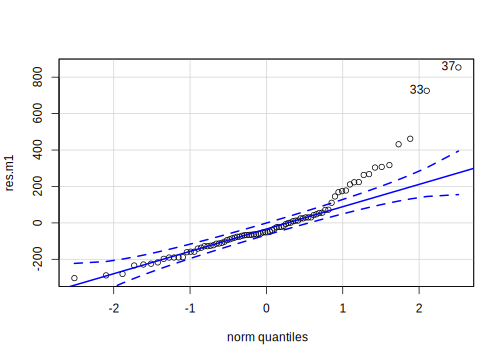
\includegraphics{Freq_CogSci_files/figure-latex/unnamed-chunk-80-1.pdf}

\begin{verbatim}
## [1] 37 33
\end{verbatim}

When the normality assumption is met, the residuals will align perfectly with the quantiles of the standard normal distribution, resulting in a straight diagonal line in the above plot. When the normality assumption is not met, the line will tend to curve away from the diagonal.

In the above case, a log transform of the data improves the normality of residuals:

\begin{Shaded}
\begin{Highlighting}[]
\NormalTok{m1log <-}\StringTok{ }\KeywordTok{lm}\NormalTok{(}\KeywordTok{log}\NormalTok{(rawRT) }\OperatorTok{~}\StringTok{ }\NormalTok{cond, bysubj)}
\KeywordTok{qqPlot}\NormalTok{(}\KeywordTok{residuals}\NormalTok{(m1log))}
\end{Highlighting}
\end{Shaded}

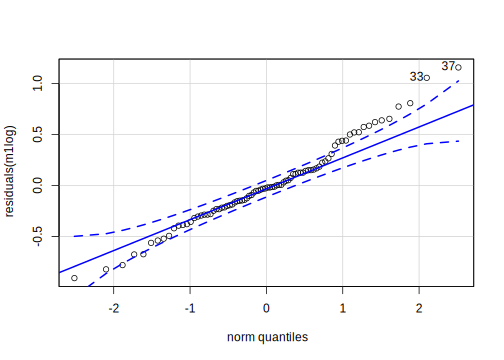
\includegraphics{Freq_CogSci_files/figure-latex/unnamed-chunk-81-1.pdf}

\begin{verbatim}
## [1] 37 33
\end{verbatim}

The estimates of the parameters are now in the log scale:

\begin{itemize}
\tightlist
\item
  The estimated grand mean processing time: \(\hat\beta_0=5.9488\).
\item
  The estimated mean object relative processing time: \(\hat\beta_0+\hat\beta_1=5.9488+0.0843=6.0331\).
\item
  The estimated mean subject relative processing time: \(\hat\beta_0-\hat\beta_1=5.9488-0.0843=5.8645\).
\end{itemize}

The model does not change, only the scale does:

\begin{equation}
\log rt = \beta_0 + \beta_1 condition  + \varepsilon 
\end{equation}

Now, the intercept and slope can be used to compute the reading time in the two conditions:

\begin{itemize}
\tightlist
\item
  Estimated mean object relative reading time: \(\hat\beta_0+\hat\beta_1=5.9488+0.0843=6.0331\).
\item
  Estimated mean subject relative reading time: \(\hat\beta_0-\hat\beta_1=5.9488-0.0843=5.8645\).
\end{itemize}

Note that because \(exp(log(rt))=rt\), to get the mean estimates on the raw ms scale, we just need to exponentiate both sides of the equation:

\begin{equation}
exp(\log rt) = exp( \beta_0 + \beta_1 condition)
\end{equation}

This approach gives us the following estimates on the ms scale:

\begin{itemize}
\tightlist
\item
  Estimated mean object relative reading time: \(exp(\hat\beta_0+\hat\beta_1)=exp(5.9488+0.0843)=417\).
\item
  Estimated mean subject relative reading time: \(exp(\hat\beta_0-\hat\beta_1)=exp(5.9488-0.0843=352\).
\end{itemize}

The difference in reading time is 417-352=65 ms (cf.~102 ms from the model using the raw scale). The larger estimate based on the raw scale is less realistic, and we will see later that the large difference between the two conditions is driven by a few extreme, influential values.

In a later chapter, we will return to the issue of which transform to choose, and what the options are that are available for different situations.

\hypertarget{from-the-paired-t-test-to-the-linear-mixed-model}{%
\section{From the paired t-test to the linear mixed model}\label{from-the-paired-t-test-to-the-linear-mixed-model}}

One interesting point to notice is that the observed t-value of the paired t-test and the t-test printed out by the linear model don't match:

\begin{Shaded}
\begin{Highlighting}[]
\KeywordTok{t.test}\NormalTok{(rawRT }\OperatorTok{~}\StringTok{ }\NormalTok{condition, bysubj, }\DataTypeTok{paired =} \OtherTok{TRUE}\NormalTok{)}\OperatorTok{$}\NormalTok{statistic}
\end{Highlighting}
\end{Shaded}

\begin{verbatim}
##     t 
## 3.109
\end{verbatim}

\begin{Shaded}
\begin{Highlighting}[]
\KeywordTok{round}\NormalTok{(}\KeywordTok{summary}\NormalTok{(m0)}\OperatorTok{$}\NormalTok{coefficients, }\DecValTok{2}\NormalTok{)[, }\KeywordTok{c}\NormalTok{(}\DecValTok{1}\OperatorTok{:}\DecValTok{3}\NormalTok{)]}
\end{Highlighting}
\end{Shaded}

\begin{verbatim}
##                  Estimate Std. Error t value
## (Intercept)         471.4      31.13   15.14
## conditionsubjgap   -102.3      44.02   -2.32
\end{verbatim}

This is because the linear model implements the unpaired (i.e., two sample) t-test:

\begin{Shaded}
\begin{Highlighting}[]
\KeywordTok{summary}\NormalTok{(}\KeywordTok{lm}\NormalTok{(rawRT }\OperatorTok{~}\StringTok{ }\NormalTok{condition, bysubj))}
\end{Highlighting}
\end{Shaded}

\begin{verbatim}
## 
## Call:
## lm(formula = rawRT ~ condition, data = bysubj)
## 
## Residuals:
##    Min     1Q Median     3Q    Max 
## -303.4 -116.4  -51.6   49.1  853.3 
## 
## Coefficients:
##                  Estimate Std. Error t value Pr(>|t|)
## (Intercept)         471.4       31.1   15.14   <2e-16
## conditionsubjgap   -102.3       44.0   -2.32    0.023
## 
## Residual standard error: 202 on 82 degrees of freedom
## Multiple R-squared:  0.0618,	Adjusted R-squared:  0.0503 
## F-statistic:  5.4 on 1 and 82 DF,  p-value: 0.0226
\end{verbatim}

\begin{Shaded}
\begin{Highlighting}[]
\KeywordTok{round}\NormalTok{(}\KeywordTok{t.test}\NormalTok{(rawRT }\OperatorTok{~}\StringTok{ }\NormalTok{condition, bysubj, }\DataTypeTok{paired =} \OtherTok{FALSE}\NormalTok{)}\OperatorTok{$}\NormalTok{statistic, }
  \DecValTok{2}\NormalTok{)}
\end{Highlighting}
\end{Shaded}

\begin{verbatim}
##    t 
## 2.32
\end{verbatim}

The paired t-test has an equivalent in the linear modeling framework: the linear mixed model. We turn next to this extension of the simple linear model. The command corresponding to the paired t-test in the linear modeling framework is:

\begin{Shaded}
\begin{Highlighting}[]
\NormalTok{m0.lmer <-}\StringTok{ }\KeywordTok{lmer}\NormalTok{(rawRT }\OperatorTok{~}\StringTok{ }\NormalTok{condition }\OperatorTok{+}\StringTok{ }\NormalTok{(}\DecValTok{1} \OperatorTok{|}\StringTok{ }\NormalTok{subject), }
\NormalTok{  bysubj)}
\KeywordTok{summary}\NormalTok{(m0.lmer)}\OperatorTok{$}\NormalTok{coefficients}
\end{Highlighting}
\end{Shaded}

\begin{verbatim}
##                  Estimate Std. Error t value
## (Intercept)         471.4      31.13  15.143
## conditionsubjgap   -102.3      32.90  -3.109
\end{verbatim}

To understand the connection between the paired t-test and the above command, it is necessary to consider how a paired t-test is assembled.

First, some background. If you have two random variables that have correlation \(\rho\), the variance of the difference between the two random variables is:

\begin{equation}
Var(X_1-X_2)=Var(X_1) + Var(X_2) - 2\times Cov(X_1, X2)
\end{equation}

\(Cov(X_1, X2)\) is the covariance between the two random variables and is defined as:

\begin{equation}
Cov(X_1, X_2) = \rho \sqrt{Var(X_1)}\sqrt{Var(X_2)}
\end{equation}

You can find the proofs of the above assertions in books like \citet{rice1995mathematical}.

As discussed earlier, a paired t-test is used when you have paired data from subject \(i=1,...,n\) in two conditions, say conditions 1 and 2. Let's write the data as two vectors \(X_{1}, X_{2}\). Because the pairs of data points are coming from the same subject, they are correlated with some correlation \(\rho\). Assume that both conditions 1 and 2 have standard deviation \(\sigma\).

To make this discussion concrete, let's generate some simulated bivariate data that are correlated. Assume that \(\sigma = 1\),
\(\rho=0.5\), and that the data are balanced.

\begin{Shaded}
\begin{Highlighting}[]
\KeywordTok{library}\NormalTok{(MASS)}
\NormalTok{samplesize <-}\StringTok{ }\DecValTok{12}
\NormalTok{mu <-}\StringTok{ }\KeywordTok{c}\NormalTok{(}\FloatTok{0.3}\NormalTok{, }\FloatTok{0.2}\NormalTok{)}
\NormalTok{rho <-}\StringTok{ }\FloatTok{0.5}
\NormalTok{stddev <-}\StringTok{ }\DecValTok{1}
\NormalTok{Sigma <-}\StringTok{ }\KeywordTok{matrix}\NormalTok{(stddev, }\DataTypeTok{nrow =} \DecValTok{2}\NormalTok{, }\DataTypeTok{ncol =} \DecValTok{2}\NormalTok{) }\OperatorTok{+}\StringTok{ }\KeywordTok{diag}\NormalTok{(}\DecValTok{2}\NormalTok{)}
\NormalTok{Sigma <-}\StringTok{ }\NormalTok{Sigma}\OperatorTok{/}\DecValTok{2}
\NormalTok{Sigma}
\end{Highlighting}
\end{Shaded}

\begin{verbatim}
##      [,1] [,2]
## [1,]  1.0  0.5
## [2,]  0.5  1.0
\end{verbatim}

\begin{Shaded}
\begin{Highlighting}[]
\CommentTok{## simulated data:}
\NormalTok{x <-}\StringTok{ }\KeywordTok{mvrnorm}\NormalTok{(}\DataTypeTok{n =}\NormalTok{ samplesize, }\DataTypeTok{mu =}\NormalTok{ mu, }\DataTypeTok{Sigma =}\NormalTok{ Sigma, }
  \DataTypeTok{empirical =} \OtherTok{TRUE}\NormalTok{)}
\KeywordTok{head}\NormalTok{(x)}
\end{Highlighting}
\end{Shaded}

\begin{verbatim}
##         [,1]    [,2]
## [1,] -0.4241 -1.1746
## [2,]  0.4285  0.1175
## [3,] -1.1445 -1.6417
## [4,]  2.1234  0.1617
## [5,] -0.9182  0.3638
## [6,]  0.6915  1.6569
\end{verbatim}

\begin{Shaded}
\begin{Highlighting}[]
\NormalTok{n <-}\StringTok{ }\NormalTok{samplesize}
\NormalTok{x1 <-}\StringTok{ }\NormalTok{x[, }\DecValTok{1}\NormalTok{]}
\NormalTok{x2 <-}\StringTok{ }\NormalTok{x[, }\DecValTok{2}\NormalTok{]}
\NormalTok{x1}
\end{Highlighting}
\end{Shaded}

\begin{verbatim}
##  [1] -0.4241  0.4285 -1.1445  2.1234 -0.9182  0.6915
##  [7] -0.3609  0.2910  0.9116  1.8084  0.4441 -0.2508
\end{verbatim}

\begin{Shaded}
\begin{Highlighting}[]
\NormalTok{x2}
\end{Highlighting}
\end{Shaded}

\begin{verbatim}
##  [1] -1.17458  0.11751 -1.64174  0.16166  0.36377
##  [6]  1.65688  1.12933 -0.26363  1.21378  1.22185
## [11] -0.41870  0.03387
\end{verbatim}

To carry out the paired t-test,
we need to know the variance of \(X_1-X_2\) because the t-statistic will be:

\begin{equation}
t_{n-1} = \frac{X_1 - X_2}{\sqrt{Var(X_1 - X_2)/n}}
\end{equation}

Now,

\begin{equation}
Var(X_1 - X_2) = \sigma^2 + \sigma^2 - 2 \rho \sigma\sigma = 2\sigma^2 (1-\rho)
\end{equation}

Now let's compute the t-statistic using the above formula. Let the actual data vectors be \(x_1, x_2\).

\begin{equation}
t_{n-1} = \frac{mean(x_1) - mean(x_2)}{\sqrt{Var(X_1 - X_2)/n}}
\end{equation}

This simplifies to:

\begin{equation}
t_{n-1} = \frac{mean(x_1) - mean(x_2)}{\sqrt{2\sigma^2(1-\rho)/n}}
\end{equation}

Now compare the paired t-test output and the by-hand calculation:

\begin{Shaded}
\begin{Highlighting}[]
\KeywordTok{t.test}\NormalTok{(x1, x2, }\DataTypeTok{paired =} \OtherTok{TRUE}\NormalTok{)}\OperatorTok{$}\NormalTok{statistic}
\end{Highlighting}
\end{Shaded}

\begin{verbatim}
##      t 
## 0.3464
\end{verbatim}

\begin{Shaded}
\begin{Highlighting}[]
\NormalTok{(}\KeywordTok{mean}\NormalTok{(x1) }\OperatorTok{-}\StringTok{ }\KeywordTok{mean}\NormalTok{(x2))}\OperatorTok{/}\KeywordTok{sqrt}\NormalTok{((}\DecValTok{2} \OperatorTok{*}\StringTok{ }\NormalTok{stddev}\OperatorTok{^}\DecValTok{2} \OperatorTok{*}\StringTok{ }\NormalTok{(}\DecValTok{1} \OperatorTok{-}\StringTok{ }\NormalTok{rho))}\OperatorTok{/}\NormalTok{n)}
\end{Highlighting}
\end{Shaded}

\begin{verbatim}
## [1] 0.3464
\end{verbatim}

The linear mixed model we present next will fit exactly the same model as in the paired t-test above. To see this, suppose we have \(i\) subjects and \(j=1,2\) conditions. For simplicity, assume that each subject sees each condition once (e.g., the by-subjects aggregated English relative clause data), so we have two data points from each subject. In other words, the data are paired.

Then, for condition 1, the dependent variable can be described by the equation:

\(y_{i1} = \beta_0 + u0_i + \varepsilon_{i1}\)

Here, \(\beta_0\) is the mean reading time, and \(\varepsilon\) is the usual residual error term. The interesting new term is \(u0_i\). This is the adjustment to the mean reading time for subject \(i\). That is, if some subject is slower than average, \(u0_i\) will be a positive number; if a subject is faster than average, then that subject's adjustment \(u0_i\) will be negative in sign; and if a subject has exactly the same reading time as the mean for all subjects, then \(u0_i\) for that subject will be 0.

Similarly, for condition 2, the dependent variable is described by the equation:

\(y_{i2} = \beta_0 + \delta + u0_i + \varepsilon_{i2}\)

Here, \(\delta\) is the additional time taken to process condition 2 (thus, this is the treatment contrast coding we saw earlier in this chapter).

If we subtract the equation for condition 2 from the equation for condition 1, the resulting equation is:

\(d_i=y_{i1} - y_{i2}= \delta + (\varepsilon_{i1}-\varepsilon_{i2})\)

The expectation of \(d_i\) is \(\delta\) because the expectation of the \(\varepsilon\) terms is 0 (we set up the model such that \(\varepsilon \sim Normal(0,\sigma)\)).

Now, assuming that the error terms are correlated with correlation \(\rho\), the result presented at the beginning of this section applies:

\begin{equation}
Var(y_{i1}-y_{i2}) = \sigma^2 + \sigma^2-2\rho\sigma^2=2\sigma^2(1-\rho)
\end{equation}

The generative distribution for \(d_i\), the pairwise differences in the two conditions, is

\begin{equation}
d \sim Normal(\delta, \sqrt{2\sigma^2(1-\rho)})
\end{equation}

But that is exactly the same standard deviation as the one used in the paired t-test.

So, the paired t-test will deliver exactly the same t-score as the above linear mixed model.

Let's check that this is true using our simulated data. In the code below, the term \texttt{(1\textbar{}subj)} is the adjustment by subject to the intercepts---the term \(u0_i\) above.

\begin{Shaded}
\begin{Highlighting}[]
\KeywordTok{library}\NormalTok{(lme4)}
\NormalTok{dat <-}\StringTok{ }\KeywordTok{data.frame}\NormalTok{(}\DataTypeTok{y =} \KeywordTok{c}\NormalTok{(x1, x2), }\DataTypeTok{cond =} \KeywordTok{rep}\NormalTok{(letters[}\DecValTok{1}\OperatorTok{:}\DecValTok{2}\NormalTok{], }
  \DataTypeTok{each =}\NormalTok{ n), }\DataTypeTok{subj =} \KeywordTok{rep}\NormalTok{(}\DecValTok{1}\OperatorTok{:}\NormalTok{n, }\DecValTok{2}\NormalTok{))}
\NormalTok{dat}\OperatorTok{$}\NormalTok{cond <-}\StringTok{ }\KeywordTok{factor}\NormalTok{(dat}\OperatorTok{$}\NormalTok{cond)}
\KeywordTok{contrasts}\NormalTok{(dat}\OperatorTok{$}\NormalTok{cond) <-}\StringTok{ }\KeywordTok{contr.sum}\NormalTok{(}\DecValTok{2}\NormalTok{)}
\KeywordTok{contrasts}\NormalTok{(dat}\OperatorTok{$}\NormalTok{cond)}
\end{Highlighting}
\end{Shaded}

\begin{verbatim}
##   [,1]
## a    1
## b   -1
\end{verbatim}

\begin{Shaded}
\begin{Highlighting}[]
\KeywordTok{summary}\NormalTok{(m <-}\StringTok{ }\KeywordTok{lmer}\NormalTok{(y }\OperatorTok{~}\StringTok{ }\NormalTok{cond }\OperatorTok{+}\StringTok{ }\NormalTok{(}\DecValTok{1} \OperatorTok{|}\StringTok{ }\NormalTok{subj), dat))}
\end{Highlighting}
\end{Shaded}

\begin{verbatim}
## Linear mixed model fit by REML ['lmerMod']
## Formula: y ~ cond + (1 | subj)
##    Data: dat
## 
## REML criterion at convergence: 65.6
## 
## Scaled residuals: 
##    Min     1Q Median     3Q    Max 
## -1.226 -0.533  0.032  0.487  1.737 
## 
## Random effects:
##  Groups   Name        Variance Std.Dev.
##  subj     (Intercept) 0.5      0.707   
##  Residual             0.5      0.707   
## Number of obs: 24, groups:  subj, 12
## 
## Fixed effects:
##             Estimate Std. Error t value
## (Intercept)    0.250      0.250    1.00
## cond1          0.050      0.144    0.35
## 
## Correlation of Fixed Effects:
##       (Intr)
## cond1 0.000
\end{verbatim}

The t-statistic from the linear mixed model is exactly the same as that from the paired t-test.

With this as background, we are ready to look at linear mixed models in detail.

\hypertarget{linear-mixed-models}{%
\section{Linear mixed models}\label{linear-mixed-models}}

We return to our subject and object relative clause data from English (Grodner and Gibson, Expt 1). First we load the data as usual, define relative clause type as a sum coded predictor, and create a new column called \texttt{so} that represents the contrast coding (\(\pm 1\) sum contrasts), and a column that holds log-transformed reading time.

\begin{Shaded}
\begin{Highlighting}[]
\NormalTok{gg05e1 <-}\StringTok{ }\KeywordTok{read.table}\NormalTok{(}\StringTok{"data/grodnergibsonE1crit.txt"}\NormalTok{, }
  \DataTypeTok{header =} \OtherTok{TRUE}\NormalTok{)}

\NormalTok{gg05e1}\OperatorTok{$}\NormalTok{so <-}\StringTok{ }\KeywordTok{ifelse}\NormalTok{(gg05e1}\OperatorTok{$}\NormalTok{condition }\OperatorTok{==}\StringTok{ "objgap"}\NormalTok{, }\DecValTok{1}\NormalTok{, }
  \DecValTok{-1}\NormalTok{)}
\NormalTok{gg05e1}\OperatorTok{$}\NormalTok{logrt <-}\StringTok{ }\KeywordTok{log}\NormalTok{(gg05e1}\OperatorTok{$}\NormalTok{rawRT)}
\end{Highlighting}
\end{Shaded}

Recall that these data have multiple measurements from each subject for each condition:

\begin{Shaded}
\begin{Highlighting}[]
\KeywordTok{t}\NormalTok{(}\KeywordTok{xtabs}\NormalTok{(}\OperatorTok{~}\NormalTok{subject }\OperatorTok{+}\StringTok{ }\NormalTok{condition, gg05e1))}
\end{Highlighting}
\end{Shaded}

\begin{verbatim}
##          subject
## condition 1 2 3 4 5 6 7 8 9 10 11 12 13 14 15 16 17 18
##   objgap  8 8 8 8 8 8 8 8 8  8  8  8  8  8  8  8  8  8
##   subjgap 8 8 8 8 8 8 8 8 8  8  8  8  8  8  8  8  8  8
##          subject
## condition 19 20 21 22 23 24 25 26 27 28 29 30 31 32 33
##   objgap   8  8  8  8  8  8  8  8  8  8  8  8  8  8  8
##   subjgap  8  8  8  8  8  8  8  8  8  8  8  8  8  8  8
##          subject
## condition 34 35 36 37 38 39 40 41 42
##   objgap   8  8  8  8  8  8  8  8  8
##   subjgap  8  8  8  8  8  8  8  8  8
\end{verbatim}

We can visualize the different responses of subjects:

\begin{verbatim}
## `geom_smooth()` using formula 'y ~ x'
\end{verbatim}

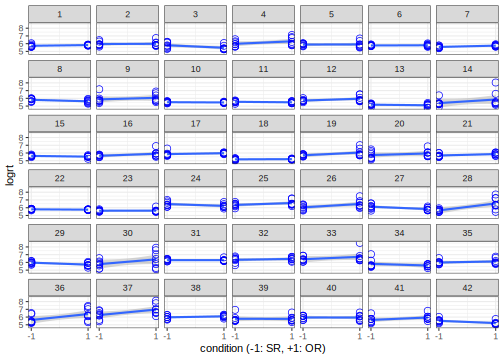
\includegraphics{Freq_CogSci_files/figure-latex/unnamed-chunk-90-1.pdf}

It's clear that different subjects have different effects of the relative clause manipulation: some slopes are positive sloping, some are flat, and some are negatively sloping. There is between-subject variability in the relative clause effect.

Given these differences between subjects, you could fit a separate linear model for each subject, collect together the intercepts and slopes for each subject, and then check if the slopes are significantly different from zero. There is a function in the package \texttt{lme4} that computes separate linear models for each subject: \emph{lmList}.

\begin{Shaded}
\begin{Highlighting}[]
\KeywordTok{library}\NormalTok{(lme4)}

\NormalTok{lmlist.fm1 <-}\StringTok{ }\KeywordTok{lmList}\NormalTok{(logrt }\OperatorTok{~}\StringTok{ }\NormalTok{so }\OperatorTok{|}\StringTok{ }\NormalTok{subject, gg05e1)}
\end{Highlighting}
\end{Shaded}

One can extract the intercept and slope estimates for each subject. For example, for subject 1:

\begin{Shaded}
\begin{Highlighting}[]
\NormalTok{lmlist.fm1}\OperatorTok{$}\StringTok{`}\DataTypeTok{1}\StringTok{`}\OperatorTok{$}\NormalTok{coefficients}
\end{Highlighting}
\end{Shaded}

\begin{verbatim}
## (Intercept)          so 
##     5.76962     0.04352
\end{verbatim}

One can plot the individual lines for each subject, as well as the fit of a simple linear model m0 for all the data taken together; this will show how each subject deviates in intercept and slope from the model m0's intercept and slope.

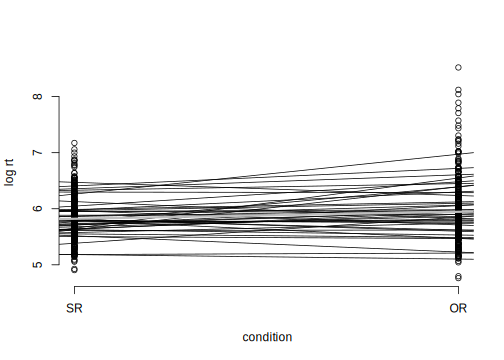
\includegraphics{Freq_CogSci_files/figure-latex/unnamed-chunk-93-1.pdf}

To find out if there is an effect of relative clause type, we simply need to check whether the slopes of the individual subjects' fitted lines taken together are significantly different from zero. A one-sample t-test will achieve this:

\begin{Shaded}
\begin{Highlighting}[]
\KeywordTok{t.test}\NormalTok{(}\KeywordTok{coef}\NormalTok{(lmlist.fm1)[}\DecValTok{2}\NormalTok{])}
\end{Highlighting}
\end{Shaded}

\begin{verbatim}
## 
## 	One Sample t-test
## 
## data:  coef(lmlist.fm1)[2]
## t = 2.8, df = 41, p-value = 0.008
## alternative hypothesis: true mean is not equal to 0
## 95 percent confidence interval:
##  0.01745 0.10658
## sample estimates:
## mean of x 
##   0.06202
\end{verbatim}

The above test is \emph{exactly} the same as the paired t-test and the varying intercepts linear mixed model that we fit in the last chapter using the by-subject aggregated data:

\begin{Shaded}
\begin{Highlighting}[]
\NormalTok{bysubj <-}\StringTok{ }\KeywordTok{aggregate}\NormalTok{(}\KeywordTok{log}\NormalTok{(rawRT) }\OperatorTok{~}\StringTok{ }\NormalTok{subject }\OperatorTok{+}\StringTok{ }\NormalTok{condition, }
\NormalTok{  mean, }\DataTypeTok{data =}\NormalTok{ gg05e1)}

\KeywordTok{colnames}\NormalTok{(bysubj)[}\DecValTok{3}\NormalTok{] <-}\StringTok{ "logrt"}

\KeywordTok{t.test}\NormalTok{(logrt }\OperatorTok{~}\StringTok{ }\NormalTok{condition, bysubj, }\DataTypeTok{paired =} \OtherTok{TRUE}\NormalTok{)}\OperatorTok{$}\NormalTok{statistic}
\end{Highlighting}
\end{Shaded}

\begin{verbatim}
##    t 
## 2.81
\end{verbatim}

\begin{Shaded}
\begin{Highlighting}[]
\CommentTok{## compare with linear mixed model:}
\KeywordTok{summary}\NormalTok{(}\KeywordTok{lmer}\NormalTok{(logrt }\OperatorTok{~}\StringTok{ }\NormalTok{condition }\OperatorTok{+}\StringTok{ }\NormalTok{(}\DecValTok{1} \OperatorTok{|}\StringTok{ }\NormalTok{subject), bysubj))}\OperatorTok{$}\NormalTok{coefficients[}\DecValTok{2}\NormalTok{, }
\NormalTok{  ]}
\end{Highlighting}
\end{Shaded}

\begin{verbatim}
##   Estimate Std. Error    t value 
##   -0.12403    0.04414   -2.81021
\end{verbatim}

The above lmList model we just fit is called \emph{repeated measures regression}. We now look at how to model unaggregated data using the linear mixed model. Incidentally, this repeated measures regression model is now only of historical interest, and useful only for understanding the linear mixed model, which is the modern standard approach.

We turn next to three main types of linear mixed model; other variants will be introduced in later chapters.

\hypertarget{model-type-1-varying-intercepts}{%
\subsection{Model type 1: Varying intercepts}\label{model-type-1-varying-intercepts}}

The \emph{linear mixed model} does something related to the above by-subject fits, but with some crucial twists, as we see below.
In the model shown below, the statement

\begin{equation}
(1 \mid \hbox{subject}) 
\end{equation}

adjusts the grand mean estimates of the intercept by a term (a number) for each subject.

\begin{Shaded}
\begin{Highlighting}[]
\NormalTok{m0.lmer <-}\StringTok{ }\KeywordTok{lmer}\NormalTok{(logrt }\OperatorTok{~}\StringTok{ }\NormalTok{so }\OperatorTok{+}\StringTok{ }\NormalTok{(}\DecValTok{1} \OperatorTok{|}\StringTok{ }\NormalTok{subject), gg05e1)}
\end{Highlighting}
\end{Shaded}

Notice that we did not aggregate the data.

Here is the abbreviated output:

\begin{verbatim}
Random effects:
 Groups   Name        Variance Std.Dev.
 subject  (Intercept) 0.09983  0.3160  
 Residual             0.14618  0.3823  
Number of obs: 672, groups:  subject, 42

Fixed effects:
            Estimate Std. Error t value
(Intercept)  5.88306    0.05094 115.497
so           0.06202    0.01475   4.205
\end{verbatim}

One thing to notice is that the coefficients (intercept and slope) of the fixed effects of the above model are identical to those in the linear model \texttt{m0} above. What is different between the linear model and the linear mixed model is the standard error. In the latter, the standard error is determined by more than one source of variance, as we explain below.

The intercept adjustments for each subject can be viewed by typing:

\begin{Shaded}
\begin{Highlighting}[]
\CommentTok{## first 10 subjects' intercept adjustments:}
\KeywordTok{ranef}\NormalTok{(m0.lmer)}\OperatorTok{$}\NormalTok{subject[, }\DecValTok{1}\NormalTok{][}\DecValTok{1}\OperatorTok{:}\DecValTok{10}\NormalTok{]}
\end{Highlighting}
\end{Shaded}

\begin{verbatim}
##  [1] -0.103928  0.077195 -0.230621  0.234198  0.008828
##  [6] -0.095363 -0.205571 -0.155371  0.075944 -0.364367
\end{verbatim}

Here is another way to summarize the adjustments to the grand mean intercept by subject. The error bars represent 95\% confidence intervals.

\begin{Shaded}
\begin{Highlighting}[]
\KeywordTok{library}\NormalTok{(lattice)}
\KeywordTok{print}\NormalTok{(}\KeywordTok{dotplot}\NormalTok{(}\KeywordTok{ranef}\NormalTok{(m0.lmer, }\DataTypeTok{condVar =} \OtherTok{TRUE}\NormalTok{)))}
\end{Highlighting}
\end{Shaded}

\begin{verbatim}
## $subject
\end{verbatim}

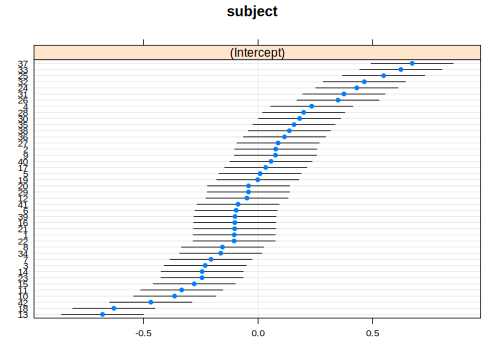
\includegraphics{Freq_CogSci_files/figure-latex/unnamed-chunk-98-1.pdf}

\hypertarget{the-formal-statement-of-the-varying-intercepts-model}{%
\subsection{The formal statement of the varying intercepts model}\label{the-formal-statement-of-the-varying-intercepts-model}}

The model \texttt{m0.lmer} above prints out the following type of linear model. \(i\) indexes subject, and \(j\) indexes items.

Once we know the subject id and the item id, we know which subject saw which condition:

\begin{Shaded}
\begin{Highlighting}[]
\KeywordTok{subset}\NormalTok{(gg05e1, subject }\OperatorTok{==}\StringTok{ }\DecValTok{1} \OperatorTok{&}\StringTok{ }\NormalTok{item }\OperatorTok{==}\StringTok{ }\DecValTok{1}\NormalTok{)}
\end{Highlighting}
\end{Shaded}

\begin{verbatim}
##   subject item condition rawRT so logrt
## 6       1    1    objgap   320  1 5.768
\end{verbatim}

The mathematical form of the linear mixed model is:

\begin{equation}
y_{ij} = \beta_0 + u_{0i}+\beta_1\times so_{ij} + \varepsilon_{ij}
\end{equation}

The \emph{only} new thing here beyond the linear model we saw earlier is the by-subject adjustment to the intercept. These by-subject adjustments to the intercept \(u_{0i}\) are assumed by lmer to come from a normal distribution centered around 0:

\begin{equation}
u_{0i} \sim Normal(0,\sigma_{u0})
\end{equation}

The ordinary linear model m0 has one intercept \(\beta_0\) for all subjects, whereas this linear mixed model with varying intercepts \texttt{m0.lmer} has a different intercept (\(\beta_0 + u_{0i}\)) for each subject \(i\).

We can visualize the adjustments for each subject to the intercepts as shown below.

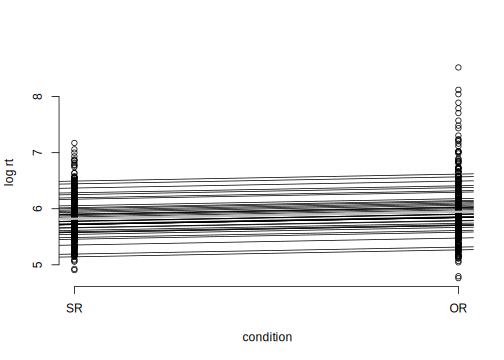
\includegraphics{Freq_CogSci_files/figure-latex/unnamed-chunk-100-1.pdf}

An important point is that in this model there are two variance components or sources of variance (cf.~the linear model, which had only one):

\begin{itemize}
\tightlist
\item
  \(u_0 \sim Normal(0,\sigma_{u0})\)
\item
  \(\varepsilon \sim Normal(0,\sigma)\)
\end{itemize}

These two standard deviations determine the standard error of the \(\beta_1\) slope parameter.

\hypertarget{model-type-2-varying-intercepts-and-slopes-without-a-correlation}{%
\subsection{Model type 2: Varying intercepts and slopes, without a correlation}\label{model-type-2-varying-intercepts-and-slopes-without-a-correlation}}

Unlike the figure associated with the \texttt{lmlist.fm1} model above, which also involves fitting separate models for each subject, the model \texttt{m0.lmer} assumes \emph{different intercepts} for each subject \emph{but the same slope}.

We can choose to fit different intercepts as well as different slopes for each subject. To achieve this, assume now that each subject's slope is also adjusted by subject:

\begin{equation}
y_{ij} = \beta_0 + u_{0i}+(\beta_1+u_{1i})\times so_{ij} + \varepsilon_{ij}
\end{equation}

That is, we additionally assume that \(u_{1i} \sim Normal(0,\sigma_{u1})\). The \texttt{lmer} notation for fitting separate intercepts and slopes is \texttt{(1+so\textbar{}\textbar{}subject)}. We will just explain what the double vertical bars represent.

\begin{Shaded}
\begin{Highlighting}[]
\NormalTok{m1.lmer <-}\StringTok{ }\KeywordTok{lmer}\NormalTok{(logrt }\OperatorTok{~}\StringTok{ }\NormalTok{so }\OperatorTok{+}\StringTok{ }\NormalTok{(}\DecValTok{1} \OperatorTok{+}\StringTok{ }\NormalTok{so }\OperatorTok{||}\StringTok{ }\NormalTok{subject), gg05e1)}
\end{Highlighting}
\end{Shaded}

The output of this model will now show that there are not two but three sources of variability. These are:

\begin{itemize}
\tightlist
\item
  \(u_0 \sim Normal(0,\sigma_{u0})\)
\item
  \(u_1 \sim Normal(0,\sigma_{u1})\)
\item
  \(\varepsilon \sim Normal(0,\sigma)\)
\end{itemize}

In particular, the model estimates the following standard deviations:

\begin{itemize}
\tightlist
\item
  \(\hat\sigma_{u0}=0.317\)
\item
  \(\hat\sigma_{u0}=0.110\)
\item
  \(\hat\sigma = 0.365\).
\end{itemize}

\begin{verbatim}
Random effects:
 Groups    Name        Variance Std.Dev.
 subject   (Intercept) 0.1006   0.317   
 subject.1 so          0.0121   0.110   
 Residual              0.1336   0.365   
Number of obs: 672, groups:  subject, 42

Fixed effects:
            Estimate Std. Error t value
(Intercept)   5.8831     0.0509  115.50
so            0.0620     0.0221    2.81
\end{verbatim}

These fits for each subject are visualized below (the gray line shows the model with a single intercept and slope, i.e., our old model \texttt{m0}):

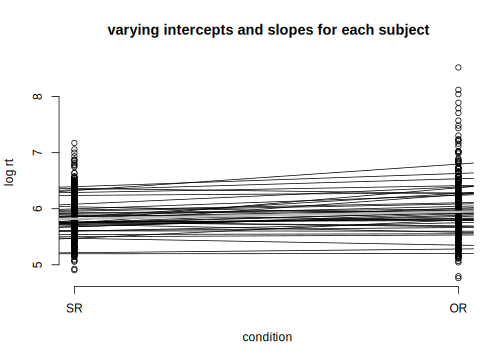
\includegraphics{Freq_CogSci_files/figure-latex/unnamed-chunk-102-1.pdf}

\hypertarget{comparing-lmlist-model-with-the-varying-intercepts-model}{%
\subsubsection{Comparing lmList model with the varying intercepts model}\label{comparing-lmlist-model-with-the-varying-intercepts-model}}

Compare this model with the \texttt{lmlist.fm1} model we fitted earlier:

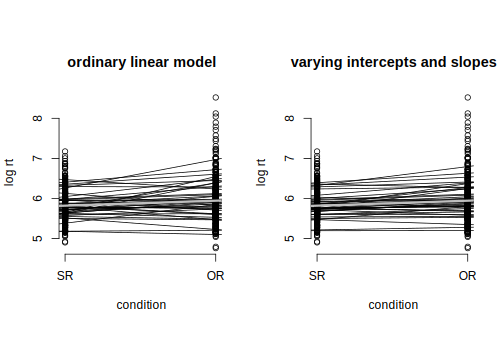
\includegraphics{Freq_CogSci_files/figure-latex/unnamed-chunk-103-1.pdf}

What is striking is that each subject's estimated best fit line is ``smooothed out'' compared to the lmList fits. This aspect of the linear mixed model is called shrinkage; we return to this point presently.

\hypertarget{visualizing-random-effects}{%
\subsubsection{Visualizing random effects}\label{visualizing-random-effects}}

As before, it is instructive to visualize the individual level adjustments to the intercept and slope:

\begin{Shaded}
\begin{Highlighting}[]
\KeywordTok{print}\NormalTok{(}\KeywordTok{dotplot}\NormalTok{(}\KeywordTok{ranef}\NormalTok{(m1.lmer, }\DataTypeTok{condVar =} \OtherTok{TRUE}\NormalTok{)))}
\end{Highlighting}
\end{Shaded}

\begin{verbatim}
## $subject
\end{verbatim}

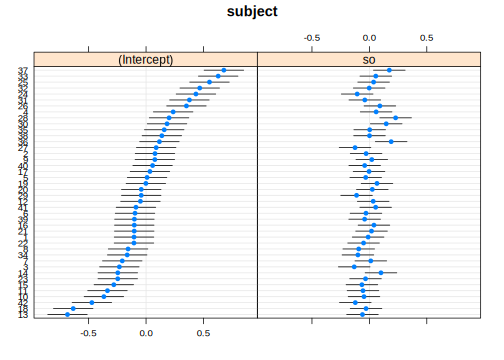
\includegraphics{Freq_CogSci_files/figure-latex/unnamed-chunk-104-1.pdf}

What this is showing is wide variability in the mean reading times between subjects, but very little variation in the slope between subjects.

\hypertarget{the-formal-statement-of-varying-intercepts-and-varying-slopes-linear-mixed-model}{%
\subsubsection{The formal statement of varying intercepts and varying slopes linear mixed model}\label{the-formal-statement-of-varying-intercepts-and-varying-slopes-linear-mixed-model}}

Here is the full statement of the varying intercept and slopes model. Again, i indexes subjects, j items.

\begin{equation}
y_{ij} = \beta_0 + u_{0i}+(\beta_1+u_{1i})\times so_{ij} + \varepsilon_{ij}
\end{equation}

As mentioned before, there are now three variance components:

\begin{itemize}
\tightlist
\item
  \(u_0 \sim Normal(0,\sigma_{u0})\)
\item
  \(u_1 \sim Normal(0,\sigma_{u1})\)
\item
  \(\varepsilon \sim Normal(0,\sigma)\)
\end{itemize}

\hypertarget{crossed-random-effects-for-subjects-and-for-items}{%
\subsubsection{Crossed random effects for subjects and for items}\label{crossed-random-effects-for-subjects-and-for-items}}

Now, one interesting fact about the varying intercepts and slopes model is that it doesn't capture all the sources of variance yet. The items also contribute sources of variance: just like subjects, items may also have different intercepts and slopes.

Notice that subjects and items are fully crossed: each subject sees each item once.

\begin{Shaded}
\begin{Highlighting}[]
\KeywordTok{head}\NormalTok{(}\KeywordTok{xtabs}\NormalTok{(}\OperatorTok{~}\NormalTok{subject }\OperatorTok{+}\StringTok{ }\NormalTok{item, gg05e1))}
\end{Highlighting}
\end{Shaded}

\begin{verbatim}
##        item
## subject 1 2 3 4 5 6 7 8 9 10 11 12 13 14 15 16
##       1 1 1 1 1 1 1 1 1 1  1  1  1  1  1  1  1
##       2 1 1 1 1 1 1 1 1 1  1  1  1  1  1  1  1
##       3 1 1 1 1 1 1 1 1 1  1  1  1  1  1  1  1
##       4 1 1 1 1 1 1 1 1 1  1  1  1  1  1  1  1
##       5 1 1 1 1 1 1 1 1 1  1  1  1  1  1  1  1
##       6 1 1 1 1 1 1 1 1 1  1  1  1  1  1  1  1
\end{verbatim}

Linear mixed model with crossed subject and items random effects can be defined with the following syntax:

\begin{Shaded}
\begin{Highlighting}[]
\NormalTok{m2.lmer <-}\StringTok{ }\KeywordTok{lmer}\NormalTok{(logrt }\OperatorTok{~}\StringTok{ }\NormalTok{so }\OperatorTok{+}\StringTok{ }\NormalTok{(}\DecValTok{1} \OperatorTok{+}\StringTok{ }\NormalTok{so }\OperatorTok{||}\StringTok{ }\NormalTok{subject) }\OperatorTok{+}\StringTok{ }
\StringTok{  }\NormalTok{(}\DecValTok{1} \OperatorTok{+}\StringTok{ }\NormalTok{so }\OperatorTok{||}\StringTok{ }\NormalTok{item), gg05e1)}
\end{Highlighting}
\end{Shaded}

Analogously to the preceding example, now there are five variance components:

\begin{verbatim}
Random effects:
 Groups    Name        Variance Std.Dev.
 subject   (Intercept) 0.10090  0.3177  
 subject.1 so          0.01224  0.1106  
 item      (Intercept) 0.00127  0.0356  
 item.1    so          0.00162  0.0402  
 Residual              0.13063  0.3614  
Number of obs: 672, groups:  subject, 42; item, 16

Fixed effects:
            Estimate Std. Error t value
(Intercept)   5.8831     0.0517  113.72
so            0.0620     0.0242    2.56
\end{verbatim}

The item intercept and slope adjustments can be visualized as well. Notice that there is a lot less item-level variation; this is often the case in planned experiments like this one, where the experimental items are carefully constructed to vary as little as possible.

\begin{Shaded}
\begin{Highlighting}[]
\KeywordTok{print}\NormalTok{(}\KeywordTok{dotplot}\NormalTok{(}\KeywordTok{ranef}\NormalTok{(m2.lmer, }\DataTypeTok{condVar =} \OtherTok{TRUE}\NormalTok{))}\OperatorTok{$}\NormalTok{item)}
\end{Highlighting}
\end{Shaded}

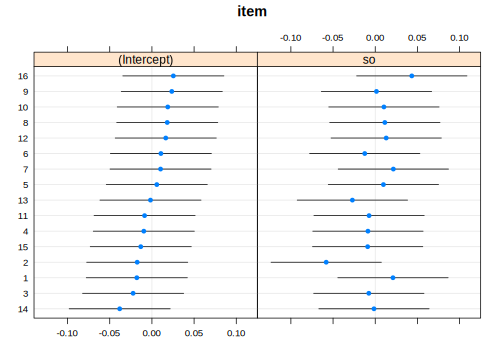
\includegraphics{Freq_CogSci_files/figure-latex/unnamed-chunk-107-1.pdf}

One thing missing in the above models is any assumption about the relationship between the intercept and slope adjustements by subject and by item. It is possible that the intercept and slope adjustments are correlated: e.g., there could be a theoretical prediction that says that the slower a subject's average reading time, the larger the difference between object and subject relative clause reading times. This kind of prediction can be tested by testing what the correlation is between the varying intercepts and slopes. We turn to this model next.

\hypertarget{model-type-3-varying-intercepts-and-varying-slopes-with-correlation}{%
\subsection{Model type 3: Varying intercepts and varying slopes, with correlation}\label{model-type-3-varying-intercepts-and-varying-slopes-with-correlation}}

A correlation can be introduced between the intercept and slope adjustments by using a single vertical bar instead of two vertical bars in the random effects structure:

\begin{Shaded}
\begin{Highlighting}[]
\NormalTok{m3.lmer <-}\StringTok{ }\KeywordTok{lmer}\NormalTok{(logrt }\OperatorTok{~}\StringTok{ }\NormalTok{so }\OperatorTok{+}\StringTok{ }\NormalTok{(}\DecValTok{1} \OperatorTok{+}\StringTok{ }\NormalTok{so }\OperatorTok{|}\StringTok{ }\NormalTok{subject) }\OperatorTok{+}\StringTok{ }\NormalTok{(}\DecValTok{1} \OperatorTok{+}\StringTok{ }
\StringTok{  }\NormalTok{so }\OperatorTok{|}\StringTok{ }\NormalTok{item), gg05e1)}
\end{Highlighting}
\end{Shaded}

\begin{verbatim}
## boundary (singular) fit: see ?isSingular
\end{verbatim}

To understand what this model is doing, we have to recall what a bivariate/multivariate distribution is.

\begin{verbatim}
Random effects:
 Groups   Name        Variance Std.Dev. Corr
 subject  (Intercept) 0.10103  0.3178       
          so          0.01228  0.1108   0.58
 item     (Intercept) 0.00172  0.0415       
          so          0.00196  0.0443   1.00 <= degeneracy
 Residual             0.12984  0.3603       
Number of obs: 672, groups:  subject, 42; item, 16

Fixed effects:
            Estimate Std. Error t value
(Intercept)   5.8831     0.0520  113.09
so            0.0620     0.0247    2.51
\end{verbatim}

The correlations (0.58 and 1.00) you see in the model output below are the correlations between the varying intercepts and slopes for subjects and for items. Notice that the variance covariance matrix for items is degenerate: its correlation is 1. This matrix cannot be inverted.

When the correlation is +1 or -1 or near these numbers, this means that the optimizer in lme4 is unable to estimate the correlation parameter, usually due to there not being enough data. If you are in such a situation, you are better off not trying to estimate this parameter with the data you have, and instead fitting one of the simpler models. We will return to this point when discussing model selection. For further discussion, see \citet{barr2013}, \citet{BatesEtAlParsimonious}, and \citet{hannesBEAP}.

\hypertarget{formal-statement-of-varying-intercepts-and-varying-slopes-linear-mixed-model-with-correlation}{%
\subsubsection{Formal statement of varying intercepts and varying slopes linear mixed model with correlation}\label{formal-statement-of-varying-intercepts-and-varying-slopes-linear-mixed-model-with-correlation}}

As usual, i indexes subjects, j items. The vector \texttt{so} is the sum-coded factor levels: +1 for object relatives and -1 for subject relatives. The only new thing in this model is the item-level effects, and the specification of the variance-covariance matrix for subjects and items, in order to include the correlation parameters.

\begin{equation}
y_{ij} = \alpha + u_{0i} + w_{0j} + (\beta + u_{1i} + w_{1j}) \times so_{ij} + \varepsilon_{ij}
\end{equation}

where \(\varepsilon_{ij} \sim Normal(0,\sigma)\) and

\begin{equation}\label{eq:covmatLM}
\Sigma_u
=
\begin{pmatrix}
\sigma _{u0}^2  & \rho _{u}\sigma _{u0}\sigma _{u1}\\
\rho _{u}\sigma _{u0}\sigma _{u1}    & \sigma _{u1}^2\\
\end{pmatrix}
\quad 
\Sigma _w
=
\begin{pmatrix}
\sigma _{w0}^2  & \rho _{w}\sigma _{w0}\sigma _{w1}\\
\rho _{w}\sigma _{w0}\sigma _{w1}    & \sigma _{w1}^2\\
\end{pmatrix}
\end{equation}

\begin{equation}\label{eq:jointpriordistLM}
\begin{pmatrix}
  u_0 \\ 
  u_1 \\
\end{pmatrix}
\sim 
\mathcal{N} \left(
\begin{pmatrix}
  0 \\
  0 \\
\end{pmatrix},
\Sigma_{u}
\right),
\quad
\begin{pmatrix}
  w_0 \\ 
  w_1 \\
\end{pmatrix}
\sim 
\mathcal{N}\left(
\begin{pmatrix}
  0 \\
  0 \\
\end{pmatrix},
\Sigma_{w}
\right)
\end{equation}

\hypertarget{visualizing-the-random-effects}{%
\subsubsection{Visualizing the random effects}\label{visualizing-the-random-effects}}

One can visualize the correlation between intercepts and slopes by subjects. The positive correlation of 0.58 between subject intercept and slope adjustments implies that slower subjects show larger effects. However, the dotplot below doesn't show a convincing pattern:

\begin{Shaded}
\begin{Highlighting}[]
\KeywordTok{print}\NormalTok{(}\KeywordTok{dotplot}\NormalTok{(}\KeywordTok{ranef}\NormalTok{(m3.lmer, }\DataTypeTok{condVar =} \OtherTok{TRUE}\NormalTok{))}\OperatorTok{$}\NormalTok{subject)}
\end{Highlighting}
\end{Shaded}

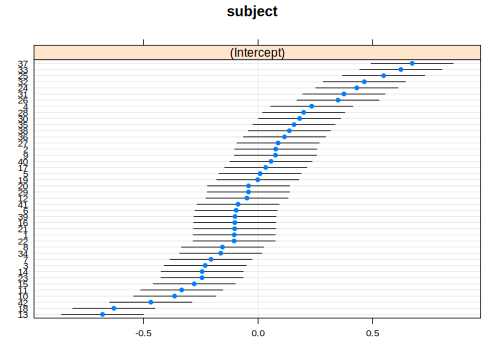
\includegraphics{Freq_CogSci_files/figure-latex/unnamed-chunk-109-1.pdf}

The correlation pattern is easier to see if we plot the slope adjustments against the intercept adjustments.

\begin{Shaded}
\begin{Highlighting}[]
\KeywordTok{plot}\NormalTok{(}\KeywordTok{ranef}\NormalTok{(m3.lmer)}\OperatorTok{$}\NormalTok{subject[, }\DecValTok{1}\NormalTok{], }\KeywordTok{ranef}\NormalTok{(m3.lmer)}\OperatorTok{$}\NormalTok{subject[, }
  \DecValTok{2}\NormalTok{], }\DataTypeTok{xlab =} \StringTok{"Intercept adjustments (subject)"}\NormalTok{, }\DataTypeTok{ylab =} \StringTok{"Slope adjustments"}\NormalTok{)}
\end{Highlighting}
\end{Shaded}

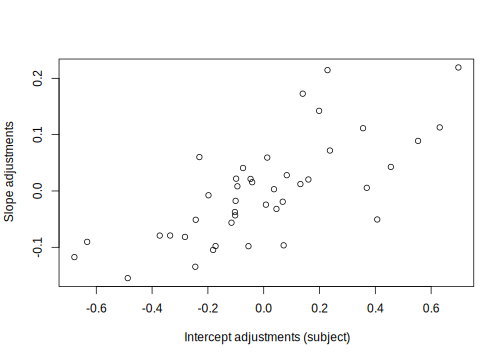
\includegraphics{Freq_CogSci_files/figure-latex/unnamed-chunk-110-1.pdf}

When we talk about hypothesis testing, we will look at what inferences we can draw from this correlation.

The dotplot showing the item-level effects shows a perfect correlation between intercept and slope adjustments, but as mentioned above these are from a degenerate variance covariance matrix and not meaningful.

\begin{Shaded}
\begin{Highlighting}[]
\KeywordTok{print}\NormalTok{(}\KeywordTok{dotplot}\NormalTok{(}\KeywordTok{ranef}\NormalTok{(m3.lmer, }\DataTypeTok{condVar =} \OtherTok{TRUE}\NormalTok{))}\OperatorTok{$}\NormalTok{item)}
\end{Highlighting}
\end{Shaded}

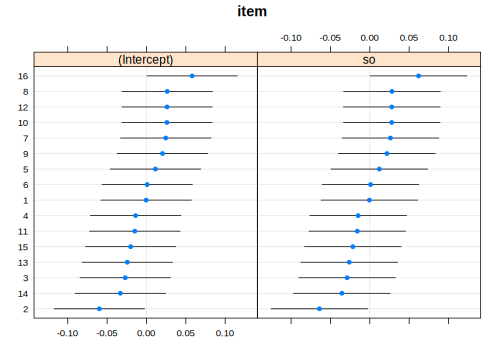
\includegraphics{Freq_CogSci_files/figure-latex/unnamed-chunk-111-1.pdf}

\hypertarget{shrinkage-in-linear-mixed-models}{%
\section{Shrinkage in linear mixed models}\label{shrinkage-in-linear-mixed-models}}

The estimate of the effect by participant is smaller than when we fit a separate linear model to the subject's data.
This is called shrinkage in linear mixed models: the individual level estimates are shrunk towards the mean slope.
The less data we have from a given subject, the greater the shrinkage.

\begin{figure}
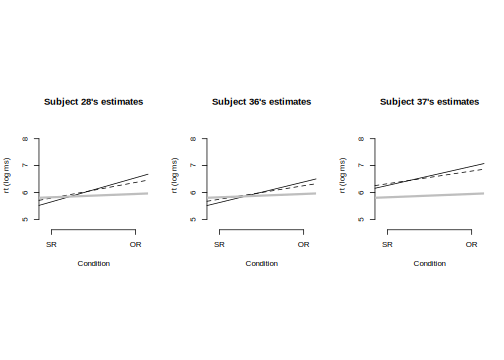
\includegraphics[width=0.75\linewidth]{Freq_CogSci_files/figure-latex/shrinkage-1} \caption{The figures show linear model fits (the grand mean estimates) for three subjects; shown are the simple linear model fit on all the data (gray line), the lmList model fit to the individual subject's data (black line), and the linear mixed model fit (the broken line). In all three subjects' models, the linear mixed model estimates are shrunk towards the grand mean (gray line) estimates.}\label{fig:shrinkage}
\end{figure}

\hypertarget{shrinkage-in-action-when-data-are-missing}{%
\subsubsection{Shrinkage in action: when data are missing}\label{shrinkage-in-action-when-data-are-missing}}

The importance and value of shrinkage becomes clear once we simulate a situation where there is some missing data. Missingness can happen in experiments, either due to lost measurements (arising from computer error or programming errors), or some other reason. To see what happens when we have missing data, let's randomly delete some data from one subject. We will randomly delete 50\% of subject 37's data:

\begin{Shaded}
\begin{Highlighting}[]
\KeywordTok{set.seed}\NormalTok{(}\DecValTok{4321}\NormalTok{)}
\CommentTok{## choose some data randomly to remove:}
\NormalTok{rand <-}\StringTok{ }\KeywordTok{rbinom}\NormalTok{(}\DecValTok{1}\NormalTok{, }\DataTypeTok{n =} \DecValTok{16}\NormalTok{, }\DataTypeTok{prob =} \FloatTok{0.5}\NormalTok{)}
\end{Highlighting}
\end{Shaded}

Here are subject 37's reading times (16 data points):

\begin{Shaded}
\begin{Highlighting}[]
\NormalTok{gg05e1[}\KeywordTok{which}\NormalTok{(gg05e1}\OperatorTok{$}\NormalTok{subject }\OperatorTok{==}\StringTok{ }\DecValTok{37}\NormalTok{), ]}\OperatorTok{$}\NormalTok{rawRT}
\end{Highlighting}
\end{Shaded}

\begin{verbatim}
##  [1]  770  536  686  578  457  487 2419  884 3365  233
## [11]  715  671 1104  281 1081  971
\end{verbatim}

Now, we randomly delete half the data:

\begin{Shaded}
\begin{Highlighting}[]
\NormalTok{gg05e1}\OperatorTok{$}\NormalTok{deletedRT <-}\StringTok{ }\NormalTok{gg05e1}\OperatorTok{$}\NormalTok{rawRT}
\NormalTok{gg05e1[}\KeywordTok{which}\NormalTok{(gg05e1}\OperatorTok{$}\NormalTok{subject }\OperatorTok{==}\StringTok{ }\DecValTok{37}\NormalTok{), ]}\OperatorTok{$}\NormalTok{deletedRT <-}\StringTok{ }\KeywordTok{ifelse}\NormalTok{(rand, }
  \OtherTok{NA}\NormalTok{, gg05e1[}\KeywordTok{which}\NormalTok{(gg05e1}\OperatorTok{$}\NormalTok{subject }\OperatorTok{==}\StringTok{ }\DecValTok{37}\NormalTok{), ]}\OperatorTok{$}\NormalTok{rawRT)}
\end{Highlighting}
\end{Shaded}

Now subject 37's estimates are going to be pretty wild, because they are based on much less data (even one extreme value can strongly influence the mean):

\begin{Shaded}
\begin{Highlighting}[]
\KeywordTok{subset}\NormalTok{(gg05e1, subject }\OperatorTok{==}\StringTok{ }\DecValTok{37}\NormalTok{)}\OperatorTok{$}\NormalTok{deletedRT}
\end{Highlighting}
\end{Shaded}

\begin{verbatim}
##  [1]  770   NA  686  578   NA   NA   NA   NA 3365  233
## [11]   NA  671 1104   NA   NA  971
\end{verbatim}

\begin{verbatim}
## [1] 6.617
\end{verbatim}

\begin{verbatim}
## [1] 0.3554
\end{verbatim}

\begin{verbatim}
## [1] 6.688
\end{verbatim}

\begin{verbatim}
## [1] 0.3884
\end{verbatim}

Now fit the hierarchical model and examine subject 37's estimates on undeleted vs deleted data:

\begin{figure}
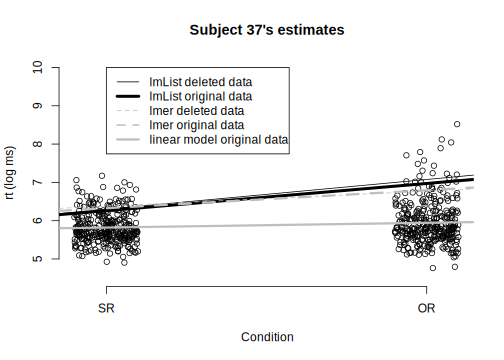
\includegraphics[width=0.75\linewidth]{Freq_CogSci_files/figure-latex/shrinkage2-1} \caption{The figures show linear model fits (the grand mean estimates) for subject 37. When using lmList, deleting data leads to very different estimates; but using lmer, deleting half the data from this subject hardly affects the individual subject's estimates.}\label{fig:shrinkage2}
\end{figure}

What we see here is that the estimates from the hierarchical model are barely affected by the missingness, but the estimates from the lmList model are heavily affected.
This means that linear mixed models will give you more robust estimates (think Type M error!) compared to no pooling models. This property of shrinkage is one reason why linear mixed models are so important in cognitive science.

\hypertarget{summary}{%
\section{Summary}\label{summary}}

\hypertarget{sec:LMExercises}{%
\section{Exercises}\label{sec:LMExercises}}

Download the data-set E1\_data.csv. Then run the following commands to load the \texttt{lme4} library and to set up your data for analysis:

\begin{Shaded}
\begin{Highlighting}[]
\KeywordTok{library}\NormalTok{(lme4)}

\CommentTok{## load data:}
\NormalTok{dat <-}\StringTok{ }\KeywordTok{read.csv}\NormalTok{(}\StringTok{"data/E1_data.csv"}\NormalTok{, }\DataTypeTok{header =} \OtherTok{TRUE}\NormalTok{)}
\CommentTok{## convert RT to milliseconds:}
\NormalTok{dat}\OperatorTok{$}\NormalTok{RT <-}\StringTok{ }\NormalTok{dat}\OperatorTok{$}\NormalTok{RT }\OperatorTok{*}\StringTok{ }\DecValTok{1000}
\CommentTok{## choose critical region:}
\NormalTok{word_n <-}\StringTok{ }\DecValTok{4}
\CommentTok{## subset critical data:}
\NormalTok{crit <-}\StringTok{ }\KeywordTok{subset}\NormalTok{(dat, Position }\OperatorTok{==}\StringTok{ }\NormalTok{word_n)}
\end{Highlighting}
\end{Shaded}

The data consist of a repeated measures experiment comparing two conditions which are labeled Type 1 and Type 2. The column Sub refers to subject id, and the column ID refers to item id. RT refers to reading time in seconds (we have converted it above to milliseconds); NA is missing data. You can ignore the other columns. This is a standard Latin square design. We will work with the data frame \texttt{crit} below.

\hypertarget{sec:LMExercisesPart1}{%
\subsection{By-subjects t-test}\label{sec:LMExercisesPart1}}

Using RT as a dependent variable, carry out the appropriate by-subjects t-test to evaluate the null hypothesis that there is no difference between the conditions labeled Type 1 and 2. Write down all the R commands needed to do the appropriate t-test, and the resulting t-value and p-value. State whether we can reject the null hypothesis given the results of the t-test; explain why.

\hypertarget{sec:LMExercisesPart2}{%
\subsection{Fitting a linear mixed model}\label{sec:LMExercisesPart2}}

Now, using the data-frame called \texttt{crit} above as the data-frame, fit a linear mixed model (called M0) with the column called Type coded as sum contrasts.

Assume varying intercepts for subjects and varying intercepts for items (varying intercepts are sometimes called random intercepts). Write down the linear mixed models command, and write down the fixed-effects estimates (Intercept and slope) along with their standard errors. State whether we can reject the null hypothesis given the results of the t-value shown in the linear mixed model output; explain why.

\hypertarget{sec:LMExercisesPart3}{%
\subsection{t-test vs.~linear mixed model}\label{sec:LMExercisesPart3}}

Why do the results of the t-test and the linear mixed model M0 differ?

\hypertarget{sec:LMExercisesPart4}{%
\subsection{Power calculation using power.t.test}\label{sec:LMExercisesPart4}}

The researcher wants to achieve 80\% statistical power in a future study. Based on the available data above, she determines that the standard error (note: not the standard deviation!) of the difference in means between the conditions Type 1 and Type 2 is 21. She has reason to believe that the true difference in means is 30 ms. What is the number of participants (to the nearest whole number) needed to achieve approximately 80\% power? Use the power.t.test function to compute your answer. Write down the \texttt{power.t.test} function specification you used, as well as the number of participants needed, based on the output of the power.t.test function.

\hypertarget{sec:LMExercisesPart5}{%
\subsection{Residuals}\label{sec:LMExercisesPart5}}

The plot below shows the distribution of the residuals from model M0 plotted against the standard normal distribution with mean 0 and standard deviation 1. Explain what the plot tells us about one of the model assumptions of the linear mixed model M0 that you fit earlier.

(You can ignore the numbers below the plot.)

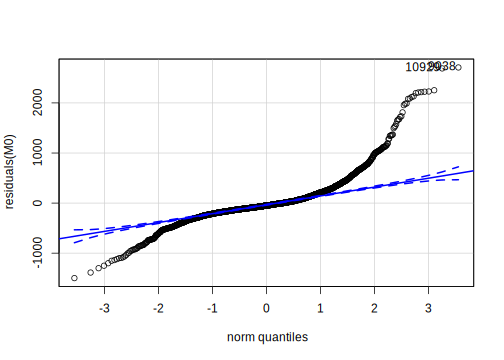
\includegraphics{Freq_CogSci_files/figure-latex/unnamed-chunk-123-1.pdf} 9038 10929
726 2544

\hypertarget{sec:LMExercisesPart6}{%
\subsection{Understanding contrast coding}\label{sec:LMExercisesPart6}}

Using only your estimates of the intercept and the slope in model M0's fixed effects output, write down the mean of the condition labeled Type 1 in the data, and the mean of the condition labeled Type 2.

\hypertarget{sec:LMExercisesPart7}{%
\subsection{Understanding the fixed-effects output}\label{sec:LMExercisesPart7}}

Suppose that the model M0's output for the fixed effects analysis were as follows. SO is a sum-coded contrast specification for the conditions labeled Type.

\begin{Shaded}
\begin{Highlighting}[]
\NormalTok{results}
\end{Highlighting}
\end{Shaded}

\begin{verbatim}
##             Estimate Std. Error t value
## (Intercept)   686.01      47.54   14.43
## SO             18.94         NA    2.00
\end{verbatim}

What is the value of the standard error of the slope (SO), which is labeled NA above?

\hypertarget{sec:LMExercisesPart8}{%
\subsection{Understanding the null hypothesis test}\label{sec:LMExercisesPart8}}

A researcher fits a linear mixed model to compare the reading times between two conditions (a) and (b), just like in the above study. Her hypothesis is that the mean for condition (a) is larger than the mean for (b). She observes that condition a has sample mean 500 ms, and condition (b) has sample mean 450 ms. She also establishes from the linear mixed model that the t-value is 1.94. The approximate p-value associated with this t-value is 0.052. Answer the following: (A) Do we have evidence against the null hypothesis and (B) do we have evidence for the particular research hypothesis that the researcher has?

The researcher runs the same analysis as above on a new data-set that has the same design as above, and now gets a p-value of 0.001. Now she has stronger evidence than in the above case where the p-value was 0.052. What does she have stronger evidence for?

\hypertarget{hypothesis-testing-using-the-likelihood-ratio-test}{%
\chapter{Hypothesis testing using the likelihood ratio test}\label{hypothesis-testing-using-the-likelihood-ratio-test}}

We started the book with the one-sample t-test. There, we had the following procedure:

\begin{itemize}
\tightlist
\item
  Given independent and identically distributed data \(y\), define a null hypothesis: \(H_0: \mu=\mu_0\)
\item
  Compute the sample mean \(\bar{y}\) and the standard error SE
\item
  Reject the null hypothesis if the absolute value of \(\bar{y}/SE\) is larger than \(2\).
\end{itemize}

Here, we turn to a closely related test: the \emph{likelihood ratio test statistic}.

\hypertarget{the-likelihood-ratio-test-the-theory}{%
\section{The likelihood ratio test: The theory}\label{the-likelihood-ratio-test-the-theory}}

Suppose that \(X_1,\dots, X_n\) are independent and normally distributed with mean \(\mu\) and standard deviation \(\sigma\) (assume for simplicity that \(\sigma\) is known).

Let the null hypothesis be \(H_0: \mu=\mu_0\) and the alternative be \(H_1: \mu\neq \mu_0\). Here, \(\mu_0\) is a number, such as \(0\).

The likelihood of the data \(y\) can be computed under the null model, in which \(\mu=\mu_0\), and under the alternative model, in which \(\mu\) has some specific alternative value. To make this concrete, imagine 10 data points being generated from a Normal(0,1).

\begin{Shaded}
\begin{Highlighting}[]
\NormalTok{y <-}\StringTok{ }\KeywordTok{rnorm}\NormalTok{(}\DecValTok{10}\NormalTok{)}
\end{Highlighting}
\end{Shaded}

We can compute the joint likelihood under a null hypothesis that \(\mu=0\):

\begin{Shaded}
\begin{Highlighting}[]
\NormalTok{likNULL <-}\StringTok{ }\KeywordTok{prod}\NormalTok{(}\KeywordTok{dnorm}\NormalTok{(y, }\DataTypeTok{mean =} \DecValTok{0}\NormalTok{, }\DataTypeTok{sd =} \DecValTok{1}\NormalTok{))}
\end{Highlighting}
\end{Shaded}

On the log scale, we would need to add the log likelihoods of each data point:

\begin{Shaded}
\begin{Highlighting}[]
\NormalTok{loglikNULL <-}\StringTok{ }\KeywordTok{sum}\NormalTok{(}\KeywordTok{dnorm}\NormalTok{(y, }\DataTypeTok{mean =} \DecValTok{0}\NormalTok{, }\DataTypeTok{sd =} \DecValTok{1}\NormalTok{, }\DataTypeTok{log =} \OtherTok{TRUE}\NormalTok{))}
\NormalTok{loglikNULL}
\end{Highlighting}
\end{Shaded}

\begin{verbatim}
## [1] -11.6
\end{verbatim}

Similarly, we can compute the log likelihood with \(\mu\) equal to the maximum likelihood estimate of \(\mu\), the sample mean.

\begin{Shaded}
\begin{Highlighting}[]
\NormalTok{loglikALT <-}\StringTok{ }\KeywordTok{sum}\NormalTok{(}\KeywordTok{dnorm}\NormalTok{(y, }\DataTypeTok{mean =} \KeywordTok{mean}\NormalTok{(y), }\DataTypeTok{sd =} \DecValTok{1}\NormalTok{, }\DataTypeTok{log =} \OtherTok{TRUE}\NormalTok{))}
\NormalTok{loglikALT}
\end{Highlighting}
\end{Shaded}

\begin{verbatim}
## [1] -11.59
\end{verbatim}

Essentially, the likelihood ratio test compares the ratio of likelihoods of the two models; on the log scale, the difference in log likelihood is taken.
The likelihood ratio test then chooses the model with the higher log likelihood, provided that the higher likelihood is high enough (we will just make this more precise).

One can specify the test in general terms as follows. Suppose that the likelihood is with respect to some parameter \(\theta\). We can evaluate the likelihood at \(\mu_0\), the null hypothesis value of the parameter, and evaluate the likelihood using the maximum likelihood estimate \(\hat\theta\) of the parameter. The likelihood ratio can then be written as follows:

\begin{equation}
\Lambda = \frac{max_{\theta\in \omega_0}(lik(\theta))}{max_{\theta\in \omega_1)}(lik(\theta))}
\end{equation}

where, \(\omega_0=\{\mu_0\}\) and \(\omega_1=\{\forall \mu \mid \mu\neq \mu_0\}\). The function max just selects the maximum value of any choices of parameter values; in the case of the null hypothesis there is only one value, \(\mu_0\). In the case of the alternative model, the maximum likelihood estimate \(\hat\theta\) is the maximum value.

Now, assuming that the data are coming from a normal distribution, the numerator of the likelihood ratio statistic is:

\begin{equation}
\frac{1}{(\sigma\sqrt{2\pi})^n} 
           exp\left( -\frac{1}{2\sigma^2} \sum_{i=1}^n (X_i - \mu_0)^2  \right)
\end{equation}

For the denominator, the MLE \(\bar{X}\) is taken as \(\mu\):

\begin{equation}
\frac{1}{(\sigma\sqrt{2\pi})^n} exp \left( -\frac{1}{2\sigma^2} \sum_{i=1}^n (X_i - \bar{X})^2 \right)
\end{equation}

The likelihood ratio statistic is then:

\begin{equation}
\Lambda = 
\frac{\frac{1}{(\sigma\sqrt{2\pi})^n} 
           exp\left( -\frac{1}{2\sigma^2} \sum_{i=1}^n (X_i - \mu_0)^2  \right)}{\frac{1}{(\sigma\sqrt{2\pi})^n} 
           exp\left( -\frac{1}{2\sigma^2} \sum_{i=1}^n (X_i - \bar{X})^2  \right)}
\end{equation}

Canceling out common terms:

\begin{equation}
\Lambda = 
\frac{exp\left( -\frac{1}{2\sigma^2} \sum_{i=1}^n (X_i - \mu_0)^2  \right)}{
        exp\left( -\frac{1}{2\sigma^2} \sum_{i=1}^n (X_i - \bar{X})^2  \right)}
\end{equation}

Taking logs:

\begin{equation}
\begin{split}
\log \Lambda =& 
\left( -\frac{1}{2\sigma^2} \sum_{i=1}^n (X_i - \mu_0)^2  \right)-\left( -\frac{1}{2\sigma^2} \sum_{i=1}^n (X_i - \bar{X})^2  \right)\\
=& -\frac{1}{2\sigma^2} \left( \sum_{i=1}^n (X_i - \mu_0)^2  -  \sum_{i=1}^n (X_i - \bar{X})^2 \right)\\
\end{split}
\end{equation}

Now, it is a standard algebraic trick to rewrite \(\sum_{i=1}^n (X_i -\mu_0)^2\) as a sum of two terms:

\begin{equation}
\sum_{i=1}^n (X_i -\mu_0)^2 = \sum_{i=1}^n (X_i - \bar{X})^2 + n(\bar{X} - \mu_0)^2 
\end{equation}

If we rearrange terms, we obtain:

\begin{equation}
\sum_{i=1}^n (X_i -\mu_0)^2 - \sum_{i=1}^n (X_i - \bar{X})^2 = n(\bar{X} - \mu_0)^2 
\end{equation}

Now, we just established above that \(\log \Lambda\) is:

\begin{equation}
\log \Lambda= -\frac{1}{2\sigma^2} \left( \sum_{i=1}^n (X_i - \mu_0)^2  -  \sum_{i=1}^n (X_i - \bar{X})^2 \right)
\end{equation}

Consider the term in the brackets:

\begin{equation}
(\sum_{i=1}^n (X_i - \mu_0)^2  -  \sum_{i=1}^n (X_i - \bar{X})^2)
\end{equation}

This can be rewritten as:

\begin{equation}
n(\bar{X} - \mu_0)^2
\end{equation}

Rewriting in this way gives us:

\begin{equation}
\ell = -\frac{1}{2\sigma^2}   n(\bar{X} - \mu_0)^2 
\end{equation}

Rearranging terms:

\begin{equation}
-2 \ell =    \frac{n(\bar{X} - \mu_0)^2 }{\sigma^2}
\end{equation}

Or even more transparently:

\begin{equation}
-2 \ell =    \frac{(\bar{X} - \mu_0)^2 }{\frac{\sigma^2}{n}}
\end{equation}

This should remind you of the t-test! Basically, just like in the t-test, what this is saying is that we reject the null when \(\mid \bar{X} - \mu_0\mid\), or negative two times the difference in log likelihood, is large!

Now we will define what it means for \(-2\ell\) to be large. We will define the \emph{likelihood ratio test statistic} as follows. Here, \(Lik(\theta)\) refers to the likelihood given some value \(\theta\) for the parameter, and
\(logLik(\theta)\) refers to the log likelihood.

\begin{equation}
\begin{split}
\Lambda =& -2\times (Lik(\theta_0)/Lik(\theta_1)) \\
\log \Lambda=& -2\times \{logLik(\theta_0)-logLik(\theta_1)\}\\
\end{split}
\end{equation}

where \(\theta_1\) and \(\theta_0\) are the estimates of \(\theta\) under the alternative and null hypotheses, respectively. The likelihood ratio test rejects \(H_0\) if \(\log \Lambda\) is sufficiently large. As the sample size approaches infinity, \(\log \Lambda\) approaches the chi-squared distribution:

\begin{equation}
\log \Lambda \rightarrow \chi_r^2  \hbox{ as }  n \rightarrow \infty
\end{equation}

where \(r\) is called the degrees of freedom and is the difference in the number of parameters under the null and alternative hypotheses.

The above result is called \emph{Wilks' theorem}. The proof of Wilks' theorem is fairly involved but you can find it in Lehmann's textbook \emph{Testing Statistical Hypotheses}.

Note that sometimes you will see the form:

\begin{equation}
 \log \Lambda = 2 \{\ell(\theta_1) - \ell(\theta_0)\}
\end{equation}

It should be clear that both statements are saying the same thing; in the second case, we are just subtracting the null hypothesis log likelihood from the alternative hypothesis log likelihood, so the negative sign disappears.

That's the theory. Let's see how the likelihood ratio test works for (a) simulated data, and (b) our running example, the English relative clause data from \citet{grodner}.

\hypertarget{a-practical-example-using-simulated-data}{%
\section{A practical example using simulated data}\label{a-practical-example-using-simulated-data}}

A practical example will make the usage of this test clear.
Let's just simulate a linear model:

\begin{Shaded}
\begin{Highlighting}[]
\NormalTok{x <-}\StringTok{ }\DecValTok{1}\OperatorTok{:}\DecValTok{10}
\NormalTok{y <-}\StringTok{ }\DecValTok{10} \OperatorTok{+}\StringTok{ }\DecValTok{20} \OperatorTok{*}\StringTok{ }\NormalTok{x }\OperatorTok{+}\StringTok{ }\KeywordTok{rnorm}\NormalTok{(}\DecValTok{10}\NormalTok{, }\DataTypeTok{sd =} \DecValTok{10}\NormalTok{)}
\end{Highlighting}
\end{Shaded}

Here, the null hypothesis that the slope is 0 is false (it has value 20). Now, we fit a null hypothesis model, without a slope:

\begin{Shaded}
\begin{Highlighting}[]
\CommentTok{## null hypothesis model:}
\NormalTok{m0 <-}\StringTok{ }\KeywordTok{lm}\NormalTok{(y }\OperatorTok{~}\StringTok{ }\DecValTok{1}\NormalTok{)}
\end{Highlighting}
\end{Shaded}

We will compare this model's log likelihood with that of the alternative model, which includes an estimate of the slope:

\begin{Shaded}
\begin{Highlighting}[]
\CommentTok{## alternative hypothesis model:}
\NormalTok{m1 <-}\StringTok{ }\KeywordTok{lm}\NormalTok{(y }\OperatorTok{~}\StringTok{ }\NormalTok{x)}
\end{Highlighting}
\end{Shaded}

The difference in log likelihood, multiplied with -2, is:

\begin{Shaded}
\begin{Highlighting}[]
\NormalTok{LogLambda <-}\StringTok{ }\DecValTok{-2} \OperatorTok{*}\StringTok{ }\NormalTok{(}\KeywordTok{logLik}\NormalTok{(m0) }\OperatorTok{-}\StringTok{ }\KeywordTok{logLik}\NormalTok{(m1))}
\CommentTok{## observed value:}
\NormalTok{LogLambda[}\DecValTok{1}\NormalTok{]}
\end{Highlighting}
\end{Shaded}

\begin{verbatim}
## [1] 34.49
\end{verbatim}

The difference in the number of parameters in the two models is one, so \(-2\log\Lambda\) has the distribution \(\chi_1^2\). Is the observed value of \(-2\log\Lambda\) unexpected under this distribution? We can calculate the probability of obtaining the likelihood ratio statistic we observed above, or a value more extreme, given the \(\chi_1^2\) distribution.

\begin{Shaded}
\begin{Highlighting}[]
\KeywordTok{pchisq}\NormalTok{(LogLambda[}\DecValTok{1}\NormalTok{], }\DataTypeTok{df =} \DecValTok{1}\NormalTok{, }\DataTypeTok{lower.tail =} \OtherTok{FALSE}\NormalTok{)}
\end{Highlighting}
\end{Shaded}

\begin{verbatim}
## [1] 4.286e-09
\end{verbatim}

Just like the critical t-value in the t-test, the critical chi-squared value here is:

\begin{Shaded}
\begin{Highlighting}[]
\CommentTok{## critical value:}
\KeywordTok{qchisq}\NormalTok{(}\FloatTok{0.95}\NormalTok{, }\DataTypeTok{df =} \DecValTok{1}\NormalTok{)}
\end{Highlighting}
\end{Shaded}

\begin{verbatim}
## [1] 3.841
\end{verbatim}

If minus two times the observed difference in log likelihood is larger than this critical value, we reject the null hypothesis.

Note that in the likelihood test above, we are comparing one nested model against another: the null hypothesis model is nested inside the alternative hypothesis model. What this means is that the alternative hypothesis model contains all the parameters in the null hypothesis model (i.e., the intercept) plus another one (the slope).

\hypertarget{a-real-life-example-the-english-relative-clause-data}{%
\section{A real-life example: The English relative clause data}\label{a-real-life-example-the-english-relative-clause-data}}

The likelihood ratio test is also the way that hypothesis testing is done with the linear mixed model. Here is how it works. Let's look again at the \citet{grodner} English relative clause data. The null hypothesis here refers to the slope parameter. When we have the sum contrast coding, the intercept \(\beta_0\) refers to the grand mean, and the slope \(\beta_1\) is the amount by which subject and object relative clause mean reading times deviate from the grand mean. Testing the null hypothesis that \(\beta_0\) is 0 amounts to testing whether there is any difference in means between the two relative clause types. This becomes clear if we consider the following.

Let object relatives be coded as \(+1\) and subject relatives as \(-1\). Then, the mean reading time \(\mu_{or}\) for object relatives in the linear mixed model is:

\begin{equation}
\mu_{or}=\beta_0 + \beta_1
\end{equation}

Similarly, the mean reading time \(\mu_{sr}\) for subject relatives is:

\begin{equation}
\mu_{sr}=\beta_0 - \beta_1
\end{equation}

If the null hypothesis is that \(\mu_{or}-\mu_{sr}=0\), then this amounts to saying that:

\begin{equation}
(\beta_0 + \beta_1)-(\beta_0 - \beta_1)=0
\end{equation}

Removing the brackets gives us:

\begin{equation}
\beta_0 + \beta_1-\beta_0 + \beta_1 = 0
\end{equation}

This yields the equation:

\begin{equation} \label{eq:nullhypsumcontrast}
2\beta_1= 0
\end{equation}

Dividing both sides of the equation by 2, we get the null hypothesis that \(\beta_1=0\).

Incidentally, if we had rescaled the contrast coding to be not \(\pm 1\) but \(\pm 1/2\), the parameter \(\beta_1\) would represent exactly the difference between the two means, and null hypothesis in equation \eqref{eq:nullhypsumcontrast} would have come out to be \(\beta_1= 0\). This is why it is sometimes better to recode the contrasts as \(\pm 1/2\) rather than \(\pm 1\). See \citet{SchadEtAlcontrasts} for details; we will discuss this in the contrast coding chapter as well.

Let's load the data, set up the contrast coding, and fit the null versus the alternative models. We will fit varying intercept and varying slopes for subject and item, without correlations for items. We don't attempt to fit the so-called ``maximal model'' here with respect to the items random effects because we would get a singularity in the variance covariance matrix.

\begin{Shaded}
\begin{Highlighting}[]
\NormalTok{gg05e1 <-}\StringTok{ }\KeywordTok{read.table}\NormalTok{(}\StringTok{"data/grodnergibsonE1crit.txt"}\NormalTok{, }
  \DataTypeTok{header =} \OtherTok{TRUE}\NormalTok{)}

\NormalTok{gg05e1}\OperatorTok{$}\NormalTok{so <-}\StringTok{ }\KeywordTok{ifelse}\NormalTok{(gg05e1}\OperatorTok{$}\NormalTok{condition }\OperatorTok{==}\StringTok{ "objgap"}\NormalTok{, }\DecValTok{1}\NormalTok{, }
  \DecValTok{-1}\NormalTok{)}
\NormalTok{gg05e1}\OperatorTok{$}\NormalTok{logrt <-}\StringTok{ }\KeywordTok{log}\NormalTok{(gg05e1}\OperatorTok{$}\NormalTok{rawRT)}

\KeywordTok{library}\NormalTok{(lme4)}
\NormalTok{m0 <-}\StringTok{ }\KeywordTok{lmer}\NormalTok{(logrt }\OperatorTok{~}\StringTok{ }\DecValTok{1} \OperatorTok{+}\StringTok{ }\NormalTok{(}\DecValTok{1} \OperatorTok{+}\StringTok{ }\NormalTok{so }\OperatorTok{|}\StringTok{ }\NormalTok{subject) }\OperatorTok{+}\StringTok{ }\NormalTok{(}\DecValTok{1} \OperatorTok{+}\StringTok{ }\NormalTok{so }\OperatorTok{||}\StringTok{ }
\StringTok{  }\NormalTok{item), gg05e1)}
\NormalTok{m1 <-}\StringTok{ }\KeywordTok{lmer}\NormalTok{(logrt }\OperatorTok{~}\StringTok{ }\DecValTok{1} \OperatorTok{+}\StringTok{ }\NormalTok{so }\OperatorTok{+}\StringTok{ }\NormalTok{(}\DecValTok{1} \OperatorTok{+}\StringTok{ }\NormalTok{so }\OperatorTok{|}\StringTok{ }\NormalTok{subject) }\OperatorTok{+}\StringTok{ }\NormalTok{(}\DecValTok{1} \OperatorTok{+}\StringTok{ }
\StringTok{  }\NormalTok{so }\OperatorTok{||}\StringTok{ }\NormalTok{item), gg05e1)}
\end{Highlighting}
\end{Shaded}

Next, we compare the two models' log likelihoods. There is a function in the \texttt{lme4} package that achieves that: the \texttt{anova} function:

\begin{Shaded}
\begin{Highlighting}[]
\KeywordTok{anova}\NormalTok{(m0, m1)}
\end{Highlighting}
\end{Shaded}

\begin{verbatim}
## refitting model(s) with ML (instead of REML)
\end{verbatim}

\begin{verbatim}
## Data: gg05e1
## Models:
## m0: logrt ~ 1 + (1 + so | subject) + ((1 | item) + (0 + so | item))
## m1: logrt ~ 1 + so + (1 + so | subject) + ((1 | item) + (0 + so | 
## m1:     item))
##    npar AIC BIC logLik deviance Chisq Df Pr(>Chisq)
## m0    7 707 739   -347      693                    
## m1    8 703 739   -343      687  6.15  1      0.013
\end{verbatim}

You can confirm from the output that the \texttt{Chisq} value shown is minus two times the difference in log likelihood of the two models. The p-value is computed using the chi-squared distribution with one degree of freedom because in the two models the difference in the number of parameters is one:

\begin{Shaded}
\begin{Highlighting}[]
\KeywordTok{round}\NormalTok{(}\KeywordTok{pchisq}\NormalTok{(}\FloatTok{5.95}\NormalTok{, }\DataTypeTok{df =} \DecValTok{1}\NormalTok{, }\DataTypeTok{lower.tail =} \OtherTok{FALSE}\NormalTok{), }\DecValTok{3}\NormalTok{)}
\end{Highlighting}
\end{Shaded}

\begin{verbatim}
## [1] 0.015
\end{verbatim}

It is common in the psycholinguistics literature to use the t-value from the linear mixed model output to conduct the hypothesis test on the slope:

\begin{Shaded}
\begin{Highlighting}[]
\KeywordTok{summary}\NormalTok{(m1)}\OperatorTok{$}\NormalTok{coefficients}
\end{Highlighting}
\end{Shaded}

\begin{verbatim}
##             Estimate Std. Error t value
## (Intercept)  5.88306    0.05176 113.669
## so           0.06202    0.02422   2.561
\end{verbatim}

The more general method for hypothesis testing is the likelihood ratio test shown above.

One can also use the likelihood ratio test to evaluate whether a variance component should be included or not. For example, is the correlation parameter justified for the subjects random effects? Recall that we had a correlation of 0.58. Is this statistically significant? One can test this in the following way:

\begin{Shaded}
\begin{Highlighting}[]
\NormalTok{m1 <-}\StringTok{ }\KeywordTok{lmer}\NormalTok{(logrt }\OperatorTok{~}\StringTok{ }\DecValTok{1} \OperatorTok{+}\StringTok{ }\NormalTok{so }\OperatorTok{+}\StringTok{ }\NormalTok{(}\DecValTok{1} \OperatorTok{+}\StringTok{ }\NormalTok{so }\OperatorTok{|}\StringTok{ }\NormalTok{subject) }\OperatorTok{+}\StringTok{ }\NormalTok{(}\DecValTok{1} \OperatorTok{+}\StringTok{ }
\StringTok{  }\NormalTok{so }\OperatorTok{||}\StringTok{ }\NormalTok{item), gg05e1)}
\NormalTok{m1NoCorr <-}\StringTok{ }\KeywordTok{lmer}\NormalTok{(logrt }\OperatorTok{~}\StringTok{ }\DecValTok{1} \OperatorTok{+}\StringTok{ }\NormalTok{so }\OperatorTok{+}\StringTok{ }\NormalTok{(}\DecValTok{1} \OperatorTok{+}\StringTok{ }\NormalTok{so }\OperatorTok{||}\StringTok{ }\NormalTok{subject) }\OperatorTok{+}\StringTok{ }
\StringTok{  }\NormalTok{(}\DecValTok{1} \OperatorTok{+}\StringTok{ }\NormalTok{so }\OperatorTok{||}\StringTok{ }\NormalTok{item), gg05e1)}
\KeywordTok{anova}\NormalTok{(m1, m1NoCorr)}
\end{Highlighting}
\end{Shaded}

\begin{verbatim}
## refitting model(s) with ML (instead of REML)
\end{verbatim}

\begin{verbatim}
## Data: gg05e1
## Models:
## m1NoCorr: logrt ~ 1 + so + ((1 | subject) + (0 + so | subject)) + ((1 | 
## m1NoCorr:     item) + (0 + so | item))
## m1: logrt ~ 1 + so + (1 + so | subject) + ((1 | item) + (0 + so | 
## m1:     item))
##          npar AIC BIC logLik deviance Chisq Df
## m1NoCorr    7 710 741   -348      696         
## m1          8 703 739   -343      687   8.7  1
##          Pr(>Chisq)
## m1NoCorr           
## m1           0.0032
\end{verbatim}

The test indicates that we can reject the null hypothesis that the correlation parameter is 0. We will return to this parameter in the chapter on simulation.

\hypertarget{sec:HypTestExercises}{%
\section{Exercises}\label{sec:HypTestExercises}}

\hypertarget{sec:HypTestExercisesChinese}{%
\subsection{Chinese relative clauses}\label{sec:HypTestExercisesChinese}}

Load the following two data-sets:

\begin{Shaded}
\begin{Highlighting}[]
\NormalTok{gibsonwu <-}\StringTok{ }\KeywordTok{read.table}\NormalTok{(}\StringTok{"data/gibsonwucrit.txt"}\NormalTok{, }\DataTypeTok{header =} \OtherTok{TRUE}\NormalTok{)}
\NormalTok{gibsonwu2 <-}\StringTok{ }\KeywordTok{read.table}\NormalTok{(}\StringTok{"data/gibsonwu2012datarepeat.txt"}\NormalTok{, }
  \DataTypeTok{header =} \OtherTok{TRUE}\NormalTok{)}
\end{Highlighting}
\end{Shaded}

The data are taken from two oexperiments that investigate (inter alia) the effect of relative clause type on reading time in Chinese. The data are from \citet{gibsonwu} and \citet{VasishthetalPLoSOne2013} respectively. The second data-set is a direct replication attempt of the first.

Chinese relative clauses are interesting theoretically because they are prenominal: the relative clause appears before the head noun. Figure \ref{fig:chineserc} shows an example.

\begin{Shaded}
\begin{Highlighting}[]
\NormalTok{knitr}\OperatorTok{::}\KeywordTok{include_graphics}\NormalTok{(}\StringTok{"figures/chineserc.png"}\NormalTok{)}
\end{Highlighting}
\end{Shaded}

\begin{figure}
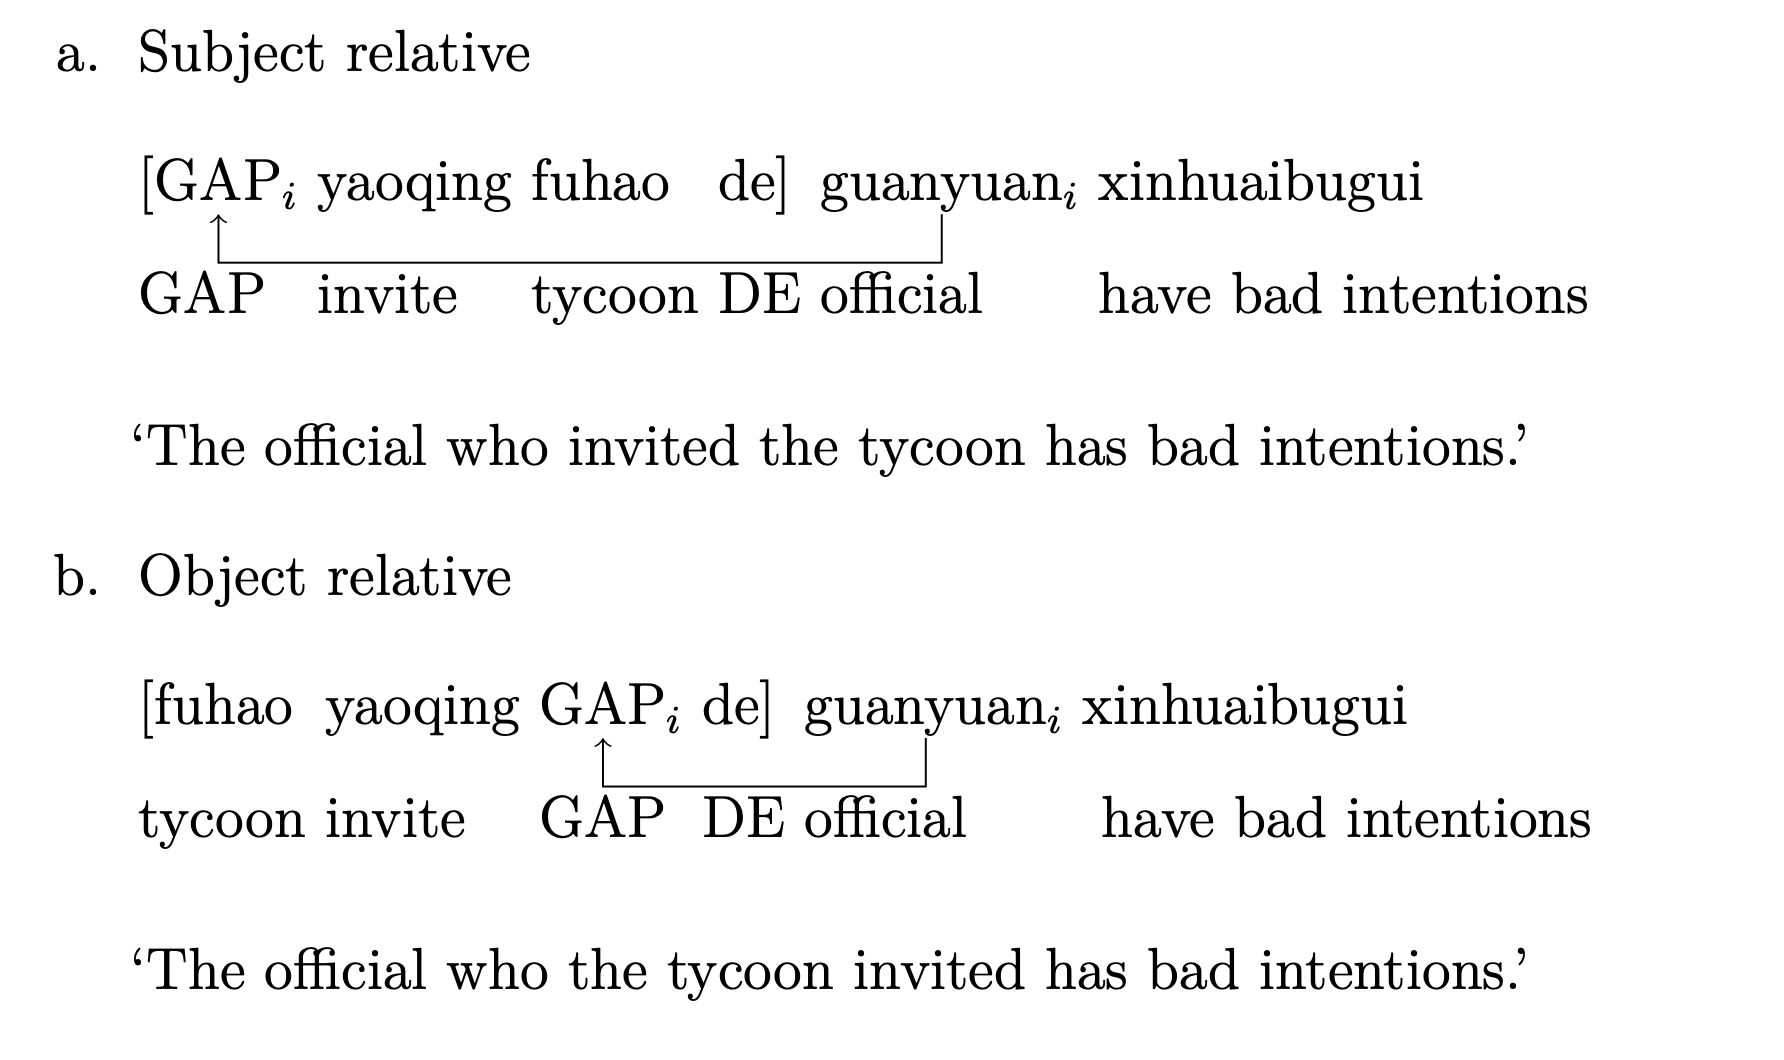
\includegraphics[width=24.78in]{figures/chineserc} \caption{\label{fig:chineserc} An example of subjects vs. object relative clauses in Chinese.}\label{fig:chinesercfig}
\end{figure}

The consequence of Chinese relative clauses being prenominal is that the distance between the gap in relative clause and the head noun is larger in subject relatives than object relatives (see Figure \ref{fig:chineserc}). \citet{hsiao03} have claimed that the larger distance in subject relatives leads to longer reading time at the head noun. Under this view, the prediction is that subject relatives are harder to process than object relatives. If this is true, this is interesting because in most other languages that have been studied, subject relatives are easier to process than object relatives; so Chinese will be a very unusual exception cross-linguistically.

The data provided are for the critical region (the head noun). The experiment method is self-paced reading, so we have reading times in milliseconds.

The research question is whether the difference in reading times between object and subject relative clauses is negative. For both data-sets, investigate this question by (a) fitting a paired t-test (by-subjects and by items), (b) fitting the most complex linear mixed model you can to the data and then interpreting the t-value, and (c) the likelihood ratio test. What can we conclude about the research question?

\hypertarget{sec:HypTestExerciseAgrmt}{%
\subsection{Agreement attraction in comprehension}\label{sec:HypTestExerciseAgrmt}}

Load the following data:

\begin{Shaded}
\begin{Highlighting}[]
\NormalTok{datE1 <-}\StringTok{ }\KeywordTok{read.table}\NormalTok{(}\StringTok{"data/dillonE1.txt"}\NormalTok{, }\DataTypeTok{header =} \OtherTok{TRUE}\NormalTok{)}
\end{Highlighting}
\end{Shaded}

The data are taken from an experiment that investigate (inter alia) the effect of number similarity between a noun and the auxiliary verb in sentences like the following. There are two levels to a factor called Int(erference): low and high.

\begin{itemize}
\tightlist
\item
  low: The key to the cabinet \emph{are} on the table
\item
  high: The key to the \emph{cabinets} \emph{are} on the table
\end{itemize}

Here, in the condition marked \emph{high}, the auxiliary verb \emph{are} is predicted to be read faster than in the condition marked \emph{low}, because the plural marking on the noun \emph{cabinets} leads the reader to think that the sentence is grammatical. (Note that both sentences are ungrammatical.) This phenomenon, where the high condition is read faster than the low condition, is called \textbf{agreement attraction}.

The data provided are for the critical region (the auxiliary verb \emph{are}). The experiment method is eyetracking; we have total reading times in milliseconds.

The research question is whether the difference in reading times between high and low conditions is negative.

\begin{itemize}
\tightlist
\item
  First, figure out which linear mixed model is appropriate for these data (varying intercepts only? varying intercepts and slopes? with or without correlations?).
\item
  Then, carry out a statistical test using (a) the paired t-test (using the t.test function), (b) the t-test of the linear mixed model, and (c) the likelihood ratio test. What is your conclusion? Is there evidence for agreement attraction in the data?
\end{itemize}

\hypertarget{sec:HypTestExerciseGramCE}{%
\subsection{The grammaticality illusion}\label{sec:HypTestExerciseGramCE}}

Load the following data-sets:

\begin{Shaded}
\begin{Highlighting}[]
\NormalTok{english <-}\StringTok{ }\KeywordTok{read.table}\NormalTok{(}\StringTok{"data/embeddingenglish.txt"}\NormalTok{, }
  \DataTypeTok{header =} \OtherTok{TRUE}\NormalTok{)}
\NormalTok{dutch <-}\StringTok{ }\KeywordTok{read.table}\NormalTok{(}\StringTok{"data/embeddingdutch.txt"}\NormalTok{, }\DataTypeTok{header =} \OtherTok{TRUE}\NormalTok{)}
\end{Highlighting}
\end{Shaded}

In an offline accuracy rating study on English double center-embedding constructions, \citet{gibsonthomas99} found that grammatical constructions (e.g., example a below) were no less acceptable than ungrammatical constructions (e.g., example b) where a middle verb phrase (e.g., was cleaning every week) was missing.

\begin{enumerate}
\def\labelenumi{(\alph{enumi})}
\item
  The apartment that the maid who the service had sent over was cleaning every week was well decorated.
\item
  *The apartment that the maid who the service had sent over --- was well decorated
\end{enumerate}

Based on these results from English, \citet{gibsonthomas99} proposed that working-memory overload leads the comprehender to forget the prediction of the upcoming verb phrase (VP), which reduces working-memory load. This came to be known as the \emph{VP-forgetting hypothesis}. The prediction is that in the word immediately following the final verb, the grammatical condition (which is coded as +1 in the data-frames) should be harder to read than the ungrammatical condition (which is coded as -1).

The data provided above test this hypothesis using self-paced reading for English \citep{VSLK08}, and for Dutch \citep{FrankEtAl2015}. The data provided are for the critical region (the noun phrase, labeled NP1, following the final verb). We have reading times in log milliseconds.

Is there support for the VP-forgetting hypothesis cross-linguistically, from English and Dutch?

\hypertarget{using-simulation-to-understand-your-model}{%
\chapter{Using simulation to understand your model}\label{using-simulation-to-understand-your-model}}

Data analysis is often taught as if the goal is to work out the p-value and make a decision: reject or fail to reject the null hypothesis. However, understanding the long-run properties of one's experiment design and statistical model under repeated sampling requires more work and thought. Specifically, it is important to understand (a) what one's model's power and Type I error properties are, and (b) whether the model we plan to fit to our data can, even in principle, recover the parameters in the model.

In order to study these properties of one's model, it is necessary to learn to simulate data that reflects our experimental design.\\
Let's think about how to simulate data given a Latin-square \(2\) condition repeated measures design. We begin with our familiar running example, the \citet{grodner} English relative clause data.

\hypertarget{a-reminder-the-maximal-linear-mixed-model}{%
\section{A reminder: The maximal linear mixed model}\label{a-reminder-the-maximal-linear-mixed-model}}

Recall the structure of the linear mixed model that can be used to fit the \citet{grodner} data. We will discuss the so-called maximal model here---varying intercepts and slopes for subject and for item, with correlations---because that is the most general case.

In the model specification below, \(i\) indexes subjects, \(j\) items. The vector \texttt{so} has the sum contrast coding as usual: object relatives are coded as +1/2 and subject relatives as -1/2. We use this coding instead of \(\pm 1\) as before, because now the slope will reflect the effect size rather than two times the effect size (see the hypothesis testing chapter).

Every row in the data-frame can be uniquely identified by the subject and item id, because this is a Latin square design and each subject sees exactly one instance of each item in a particular condition.

\begin{equation}
y_{ij} = \beta_0 + u_{0i} + w_{0j} + (\beta_1 + u_{1i} + w_{1j}) \times so_{ij} + \varepsilon_{ij}
\end{equation}

where \(\varepsilon_{ij} \sim Normal(0,\sigma)\) and

\begin{equation}\label{eq:covmatsimulations}
\Sigma_u
=
\begin{pmatrix}
\sigma _{u0}^2  & \rho _{u}\sigma _{u0}\sigma _{u1}\\
\rho _{u}\sigma _{u0}\sigma _{u1}    & \sigma _{u1}^2\\
\end{pmatrix}
\quad 
\Sigma _w
=
\begin{pmatrix}
\sigma _{w0}^2  & \rho _{w}\sigma _{w0}\sigma _{w1}\\
\rho _{w}\sigma _{w0}\sigma _{w1}    & \sigma _{w1}^2\\
\end{pmatrix}
\end{equation}

\begin{equation}\label{eq:jointpriordistsimulation}
\begin{pmatrix}
  u_0 \\ 
  u_1 \\
\end{pmatrix}
\sim 
\mathcal{N} \left(
\begin{pmatrix}
  0 \\
  0 \\
\end{pmatrix},
\Sigma_{u}
\right),
\quad
\begin{pmatrix}
  w_0 \\ 
  w_1 \\
\end{pmatrix}
\sim 
\mathcal{N}\left(
\begin{pmatrix}
  0 \\
  0 \\
\end{pmatrix},
\Sigma_{w}
\right)
\end{equation}

\(\beta_0\) and \(\beta_1\) are the intercept and slope, representing the grand mean and the deviation from the grand mean in each condition. \(u\) are the subject level adjustments, and \(w\) the item level adjustments to the intercept and slope.\\
The above mathematical model expresses a generative process. In order to produce simulated data using the above process, we have to decide on some parameter values. We do this by estimating the parameters from the \citet{grodner} study.

\hypertarget{obtain-estimates-from-a-previous-study}{%
\section{Obtain estimates from a previous study}\label{obtain-estimates-from-a-previous-study}}

First we load and prepare the relative clause data for data analysis.

\begin{Shaded}
\begin{Highlighting}[]
\NormalTok{gg05e1 <-}\StringTok{ }\KeywordTok{read.table}\NormalTok{(}\StringTok{"data/grodnergibsonE1crit.txt"}\NormalTok{, }
  \DataTypeTok{header =} \OtherTok{TRUE}\NormalTok{)}


\NormalTok{gg05e1}\OperatorTok{$}\NormalTok{so <-}\StringTok{ }\KeywordTok{ifelse}\NormalTok{(gg05e1}\OperatorTok{$}\NormalTok{condition }\OperatorTok{==}\StringTok{ "objgap"}\NormalTok{, }\DecValTok{1}\OperatorTok{/}\DecValTok{2}\NormalTok{, }
  \DecValTok{-1}\OperatorTok{/}\DecValTok{2}\NormalTok{)}
\NormalTok{gg05e1}\OperatorTok{$}\NormalTok{logrt <-}\StringTok{ }\KeywordTok{log}\NormalTok{(gg05e1}\OperatorTok{$}\NormalTok{rawRT)}
\end{Highlighting}
\end{Shaded}

Next, fit the so-called maximal model. We will ignore the singularity warning as it won't affect us in our simulations.

\begin{Shaded}
\begin{Highlighting}[]
\KeywordTok{library}\NormalTok{(lme4)}
\NormalTok{m<-}\KeywordTok{lmer}\NormalTok{(logrt }\OperatorTok{~}\StringTok{ }\NormalTok{so }\OperatorTok{+}\StringTok{ }
\StringTok{          }\NormalTok{(}\DecValTok{1}\OperatorTok{+}\NormalTok{so}\OperatorTok{|}\NormalTok{subject) }\OperatorTok{+}\StringTok{ }
\StringTok{          }\NormalTok{(}\DecValTok{1}\OperatorTok{+}\NormalTok{so}\OperatorTok{|}\NormalTok{item), }
        \DataTypeTok{data=}\NormalTok{gg05e1,}
        \CommentTok{## "switch off" warnings:}
        \DataTypeTok{control=}\KeywordTok{lmerControl}\NormalTok{(}\DataTypeTok{calc.derivs=}\OtherTok{FALSE}\NormalTok{))}
\end{Highlighting}
\end{Shaded}

The model summary shows that we can reject the null hypothesis of no difference in relative clauses:

\begin{Shaded}
\begin{Highlighting}[]
\KeywordTok{summary}\NormalTok{(m)}\OperatorTok{$}\NormalTok{coefficients}
\end{Highlighting}
\end{Shaded}

\begin{verbatim}
##             Estimate Std. Error t value
## (Intercept)    5.883    0.05202 113.082
## so             0.124    0.04932   2.515
\end{verbatim}

Let's focus on that effect for our power analysis. What is the prospective power of detecting this effect \emph{for a future study}? Note that we never compute power for an existing study---that is called post-hoc power and is a pointless quantity to compute because once the p-value is known, the power is just a transformation of the p-value \citep{hoenigheisey}.

What we are doing below will \emph{look} like post-hoc power because we are using existing data to compute power. However, what is crucially different in our approach is that (a) we remain unsure about the true effect, (b) we are making a statement about what the power properties would be \emph{if we ran the same study again}, with new subjects, but in the same environment (lab, etc.). We are not making any claim about the power properties of the \emph{current} experiment; that ship has already sailed, the data are already at hand! Once the data are analyzed, it's too late to compute power for that particular data-set. A power analysis is only relevant for a design to be run in the future.

\hypertarget{decide-on-a-range-of-plausible-values-of-the-effect-size}{%
\section{Decide on a range of plausible values of the effect size}\label{decide-on-a-range-of-plausible-values-of-the-effect-size}}

Notice that the effect in milliseconds is relatively large, given the estimates from similar phenomena in reading studies in psycholinguistics \citep{JaegerEngelmannVasishth2017}:

\begin{Shaded}
\begin{Highlighting}[]
\NormalTok{b0 <-}\StringTok{ }\KeywordTok{summary}\NormalTok{(m)}\OperatorTok{$}\NormalTok{coefficients[}\DecValTok{1}\NormalTok{, }\DecValTok{1}\NormalTok{]}
\NormalTok{b1 <-}\StringTok{ }\KeywordTok{summary}\NormalTok{(m)}\OperatorTok{$}\NormalTok{coefficients[}\DecValTok{2}\NormalTok{, }\DecValTok{1}\NormalTok{]}
\CommentTok{## effect estimate in log ms:}
\NormalTok{b1}
\end{Highlighting}
\end{Shaded}

\begin{verbatim}
## [1] 0.124
\end{verbatim}

\begin{Shaded}
\begin{Highlighting}[]
\CommentTok{## effect estimate in ms:}
\KeywordTok{exp}\NormalTok{(b0 }\OperatorTok{+}\StringTok{ }\NormalTok{b1 }\OperatorTok{*}\StringTok{ }\NormalTok{(}\FloatTok{0.5}\NormalTok{)) }\OperatorTok{-}\StringTok{ }\KeywordTok{exp}\NormalTok{(b0 }\OperatorTok{+}\StringTok{ }\NormalTok{b1 }\OperatorTok{*}\StringTok{ }\NormalTok{(}\OperatorTok{-}\FloatTok{0.5}\NormalTok{))}
\end{Highlighting}
\end{Shaded}

\begin{verbatim}
## [1] 44.54
\end{verbatim}

But the standard errors tell us that the effect could be as small or as large as the following values:

\begin{Shaded}
\begin{Highlighting}[]
\NormalTok{b1_stderr <-}\StringTok{ }\KeywordTok{summary}\NormalTok{(m)}\OperatorTok{$}\NormalTok{coefficients[}\DecValTok{2}\NormalTok{, }\DecValTok{2}\NormalTok{]}
\NormalTok{lower <-}\StringTok{ }\NormalTok{b1 }\OperatorTok{-}\StringTok{ }\DecValTok{2} \OperatorTok{*}\StringTok{ }\NormalTok{b1_stderr}
\NormalTok{upper <-}\StringTok{ }\NormalTok{b1 }\OperatorTok{+}\StringTok{ }\DecValTok{2} \OperatorTok{*}\StringTok{ }\NormalTok{b1_stderr}
\NormalTok{lower}
\end{Highlighting}
\end{Shaded}

\begin{verbatim}
## [1] 0.02539
\end{verbatim}

\begin{Shaded}
\begin{Highlighting}[]
\NormalTok{upper}
\end{Highlighting}
\end{Shaded}

\begin{verbatim}
## [1] 0.2227
\end{verbatim}

The above range 0.03 and 0.22 arises because the range of plausible effect sizes is between \(\hat\beta_1 \pm 2SE\) on the log ms scale.

On the ms scale, the range is:

\begin{Shaded}
\begin{Highlighting}[]
\KeywordTok{exp}\NormalTok{(b0 }\OperatorTok{+}\StringTok{ }\NormalTok{lower }\OperatorTok{*}\StringTok{ }\NormalTok{(}\FloatTok{0.5}\NormalTok{)) }\OperatorTok{-}\StringTok{ }\KeywordTok{exp}\NormalTok{(b0 }\OperatorTok{+}\StringTok{ }\NormalTok{lower }\OperatorTok{*}\StringTok{ }\NormalTok{(}\OperatorTok{-}\FloatTok{0.5}\NormalTok{))}
\end{Highlighting}
\end{Shaded}

\begin{verbatim}
## [1] 9.113
\end{verbatim}

\begin{Shaded}
\begin{Highlighting}[]
\KeywordTok{exp}\NormalTok{(b0 }\OperatorTok{+}\StringTok{ }\NormalTok{upper }\OperatorTok{*}\StringTok{ }\NormalTok{(}\FloatTok{0.5}\NormalTok{)) }\OperatorTok{-}\StringTok{ }\KeywordTok{exp}\NormalTok{(b0 }\OperatorTok{+}\StringTok{ }\NormalTok{upper }\OperatorTok{*}\StringTok{ }\NormalTok{(}\OperatorTok{-}\FloatTok{0.5}\NormalTok{))}
\end{Highlighting}
\end{Shaded}

\begin{verbatim}
## [1] 80.09
\end{verbatim}

On the ms scale we see that that's a \emph{lot} of uncertainty in the effect size! With some experience, you will come to recognize that such a wide confidence bound is a sign of low power. We will just establish the prospective power properties of this study in a minute.

We can take the above uncertainty of the \(\hat\beta_1\) estimator into account (on the log ms scale---remember that the model is based on log rt) by assuming that the effect has the following uncertainty on the log ms scale:

\begin{equation}
\beta_1 \sim Normal(0.12,0.05)
\end{equation}

Here, we are doing something that is, strictly speaking, Bayesian in thinking. We are describing our uncertainty about the true effect from the best estimate we have---existing data. To talk about the uncertainty, we are (ab)using the 95\% confidence interval (treating it like its telling us the range of plausible values). Recall that strictly speaking, in the frequentist paradigm, one cannot talk about the probability distribution of the effect size---in frequentist theory, the true value of the parameter is a point value, it has no distribution. The range \(\hat\beta_1 \pm 2\times SE\) refers to the estimated mean of the sampling distribution of the sample means, and to the standard deviation of this sampling distribution. Thus, strictly speaking, this range does not reflect our uncertainty about the true parameter's value. Having said this, we are going to use the effect estimates from our model fit as a starting point for our power analysis because this is the best information we have so far about the English relative clause design.

\hypertarget{extract-parameter-estimates}{%
\section{Extract parameter estimates}\label{extract-parameter-estimates}}

Next, in preparation for the power analysis, we extract all the parameter estimates from the model we have fit above. The parameters are:

\begin{itemize}
\tightlist
\item
  The two fixed effects (the \(\beta\) parameters)
\item
  The residuals' standard deviation
\item
  The standard deviations of the subject intercept and slope adjustments, and the corresponding correlation matrix.
\item
  The standard deviations of the item intercept and slope adjustments, and the corresponding correlation matrix.
\end{itemize}

The correlation matrices and the subject/item random effects standard deviations are used to assemble the variance covariance matrix; this is done using the \texttt{sdcor2cov} function from the \texttt{SIN} package; recall the discussion in chapter 1. For the variance covariance matrix for items random effects, we use an intermediate value of 0.5 for the correlation parameter because the linear mixed model was unable to estimate the parameter.

\begin{Shaded}
\begin{Highlighting}[]
\CommentTok{## extract parameter estimates:}
\NormalTok{beta <-}\StringTok{ }\KeywordTok{round}\NormalTok{(}\KeywordTok{summary}\NormalTok{(m)}\OperatorTok{$}\NormalTok{coefficients[, }\DecValTok{1}\NormalTok{], }\DecValTok{4}\NormalTok{)}
\NormalTok{sigma_e <-}\StringTok{ }\KeywordTok{round}\NormalTok{(}\KeywordTok{attr}\NormalTok{(}\KeywordTok{VarCorr}\NormalTok{(m), }\StringTok{"sc"}\NormalTok{), }\DecValTok{2}\NormalTok{)}
\NormalTok{subj_ranefsd <-}\StringTok{ }\KeywordTok{round}\NormalTok{(}\KeywordTok{attr}\NormalTok{(}\KeywordTok{VarCorr}\NormalTok{(m)}\OperatorTok{$}\NormalTok{subject, }\StringTok{"stddev"}\NormalTok{), }
  \DecValTok{4}\NormalTok{)}
\NormalTok{subj_ranefcorr <-}\StringTok{ }\KeywordTok{round}\NormalTok{(}\KeywordTok{attr}\NormalTok{(}\KeywordTok{VarCorr}\NormalTok{(m)}\OperatorTok{$}\NormalTok{subject, }\StringTok{"corr"}\NormalTok{), }
  \DecValTok{1}\NormalTok{)}

\CommentTok{## assemble variance-covariance matrix for subjects:}
\NormalTok{Sigma_u <-}\StringTok{ }\NormalTok{SIN}\OperatorTok{::}\KeywordTok{sdcor2cov}\NormalTok{(}\DataTypeTok{stddev =}\NormalTok{ subj_ranefsd, }\DataTypeTok{corr =}\NormalTok{ subj_ranefcorr)}
\CommentTok{## check that the matrix can be inverted:}
\KeywordTok{solve}\NormalTok{(Sigma_u)}
\end{Highlighting}
\end{Shaded}

\begin{verbatim}
##             (Intercept)     so
## (Intercept)       15.46 -13.31
## so               -13.31  31.82
\end{verbatim}

\begin{Shaded}
\begin{Highlighting}[]
\NormalTok{item_ranefsd <-}\StringTok{ }\KeywordTok{round}\NormalTok{(}\KeywordTok{attr}\NormalTok{(}\KeywordTok{VarCorr}\NormalTok{(m)}\OperatorTok{$}\NormalTok{item, }\StringTok{"stddev"}\NormalTok{), }
  \DecValTok{4}\NormalTok{)}
\NormalTok{item_ranefcorr <-}\StringTok{ }\KeywordTok{round}\NormalTok{(}\KeywordTok{attr}\NormalTok{(}\KeywordTok{VarCorr}\NormalTok{(m)}\OperatorTok{$}\NormalTok{item, }\StringTok{"corr"}\NormalTok{), }
  \DecValTok{1}\NormalTok{)}

\CommentTok{## assemble variance matrix for items: ## this won't}
\CommentTok{## work:}
\CommentTok{## Sigma_w<-SIN::sdcor2cov(stddev=item_ranefsd,}
\CommentTok{## corr=item_ranefcorr) solve(Sigma_w) choose some}
\CommentTok{## intermediate values for correlations:}
\NormalTok{corr_matrix <-}\StringTok{ }\NormalTok{(}\KeywordTok{diag}\NormalTok{(}\DecValTok{2}\NormalTok{) }\OperatorTok{+}\StringTok{ }\KeywordTok{matrix}\NormalTok{(}\KeywordTok{rep}\NormalTok{(}\DecValTok{1}\NormalTok{, }\DecValTok{4}\NormalTok{), }\DataTypeTok{ncol =} \DecValTok{2}\NormalTok{))}\OperatorTok{/}\DecValTok{2}

\NormalTok{Sigma_w <-}\StringTok{ }\NormalTok{SIN}\OperatorTok{::}\KeywordTok{sdcor2cov}\NormalTok{(}\DataTypeTok{stddev =}\NormalTok{ item_ranefsd, }\DataTypeTok{corr =}\NormalTok{ corr_matrix)}
\CommentTok{## matrix inverts:}
\KeywordTok{solve}\NormalTok{(Sigma_w)}
\end{Highlighting}
\end{Shaded}

\begin{verbatim}
##        [,1]   [,2]
## [1,]  774.2 -181.3
## [2,] -181.3  169.9
\end{verbatim}

\hypertarget{define-a-function-for-generating-data}{%
\section{Define a function for generating data}\label{define-a-function-for-generating-data}}

Next, we define a function that generates repeated measures data given the parameter estimates. The basic idea here is the following.

\begin{itemize}
\tightlist
\item
  First, create a data-frame that represents a Latin-square design.
\item
  Then, given the condition id, and the subject and item ids in each row of the data frame, generate data row-by-row.
\end{itemize}

We explain these steps next.

\hypertarget{generate-a-latin-square-design}{%
\subsection{Generate a Latin-square design}\label{generate-a-latin-square-design}}

First, consider how one can create a Latin-square design. Suppose we have four items and four subjects. For such an experiment, we would create two groups, g1 and g2, with the following layout.

\begin{Shaded}
\begin{Highlighting}[]
\NormalTok{nitem <-}\StringTok{ }\DecValTok{4}
\NormalTok{nsubj <-}\StringTok{ }\DecValTok{4}

\NormalTok{g1 <-}\StringTok{ }\KeywordTok{data.frame}\NormalTok{(}\DataTypeTok{item =} \DecValTok{1}\OperatorTok{:}\NormalTok{nitem, }\DataTypeTok{cond =} \KeywordTok{rep}\NormalTok{(}\KeywordTok{c}\NormalTok{(}\StringTok{"a"}\NormalTok{, }
  \StringTok{"b"}\NormalTok{), nitem}\OperatorTok{/}\DecValTok{2}\NormalTok{))}
\NormalTok{g2 <-}\StringTok{ }\KeywordTok{data.frame}\NormalTok{(}\DataTypeTok{item =} \DecValTok{1}\OperatorTok{:}\NormalTok{nitem, }\DataTypeTok{cond =} \KeywordTok{rep}\NormalTok{(}\KeywordTok{c}\NormalTok{(}\StringTok{"b"}\NormalTok{, }
  \StringTok{"a"}\NormalTok{), nitem}\OperatorTok{/}\DecValTok{2}\NormalTok{))}
\NormalTok{g1}
\end{Highlighting}
\end{Shaded}

\begin{verbatim}
##   item cond
## 1    1    a
## 2    2    b
## 3    3    a
## 4    4    b
\end{verbatim}

\begin{Shaded}
\begin{Highlighting}[]
\NormalTok{g2}
\end{Highlighting}
\end{Shaded}

\begin{verbatim}
##   item cond
## 1    1    b
## 2    2    a
## 3    3    b
## 4    4    a
\end{verbatim}

Half the total number of subjects will be assigned to group 1 and half to group 2:

\begin{Shaded}
\begin{Highlighting}[]
\CommentTok{## assemble data frame:}
\NormalTok{gp1 <-}\StringTok{ }\NormalTok{g1[}\KeywordTok{rep}\NormalTok{(}\KeywordTok{seq_len}\NormalTok{(}\KeywordTok{nrow}\NormalTok{(g1)), nsubj}\OperatorTok{/}\DecValTok{2}\NormalTok{), ]}
\NormalTok{gp2 <-}\StringTok{ }\NormalTok{g2[}\KeywordTok{rep}\NormalTok{(}\KeywordTok{seq_len}\NormalTok{(}\KeywordTok{nrow}\NormalTok{(g2)), nsubj}\OperatorTok{/}\DecValTok{2}\NormalTok{), ]}

\NormalTok{simdat <-}\StringTok{ }\KeywordTok{rbind}\NormalTok{(gp1, gp2)}

\CommentTok{## add subject column:}
\NormalTok{simdat}\OperatorTok{$}\NormalTok{subj <-}\StringTok{ }\KeywordTok{rep}\NormalTok{(}\DecValTok{1}\OperatorTok{:}\NormalTok{nsubj, }\DataTypeTok{each =}\NormalTok{ nitem)}
\end{Highlighting}
\end{Shaded}

Finally, the contrast coding for each row in the data-frame is set up:

\begin{Shaded}
\begin{Highlighting}[]
\CommentTok{## add contrast coding:}
\NormalTok{simdat}\OperatorTok{$}\NormalTok{so <-}\StringTok{ }\KeywordTok{ifelse}\NormalTok{(simdat}\OperatorTok{$}\NormalTok{cond }\OperatorTok{==}\StringTok{ "a"}\NormalTok{, }\DecValTok{-1}\OperatorTok{/}\DecValTok{2}\NormalTok{, }\DecValTok{1}\OperatorTok{/}\DecValTok{2}\NormalTok{)}
\end{Highlighting}
\end{Shaded}

\hypertarget{generate-data-row-by-row}{%
\subsection{Generate data row-by-row}\label{generate-data-row-by-row}}

Then, we proceed row-by-row in this data frame, and generate data for each subject, item, and condition. For example, the first row of our simulated data-set has subject id:

\begin{Shaded}
\begin{Highlighting}[]
\NormalTok{simdat[}\DecValTok{1}\NormalTok{, ]}\OperatorTok{$}\NormalTok{subj}
\end{Highlighting}
\end{Shaded}

\begin{verbatim}
## [1] 1
\end{verbatim}

Similarly, the first row has item id:

\begin{Shaded}
\begin{Highlighting}[]
\NormalTok{simdat[}\DecValTok{1}\NormalTok{, ]}\OperatorTok{$}\NormalTok{item}
\end{Highlighting}
\end{Shaded}

\begin{verbatim}
## [1] 1
\end{verbatim}

The first row's condition coding is:

\begin{Shaded}
\begin{Highlighting}[]
\NormalTok{simdat[}\DecValTok{1}\NormalTok{, ]}\OperatorTok{$}\NormalTok{so}
\end{Highlighting}
\end{Shaded}

\begin{verbatim}
## [1] -0.5
\end{verbatim}

These three pieces of information are what we need to generate data for the first row. Recall that the model for subject \(i\) and item \(j\) in condition \texttt{so} is

\begin{equation}
\beta_0 + u_{0i} + w_{0j} + (\beta+1 + u_{1i} + w_{1j})\times so + \varepsilon \hbox{ where } \varepsilon \sim N(0,\sigma)
\end{equation}

The terms u0, w0, and u1, w1, which are the adjustments to the intercepts and slopes by subject and item, are stored in two matrices that are generated randomly each time that we simulate new subjects/items. Recall from chapter 1 how bivariate data are generated. The intercept and slope adjustments will be generated using the \texttt{mvrnorm} function in the MASS library. For example, given the variance covariance matrix for subjects \texttt{Sigma\_u} that we created above, the subject random effects (intercept and slope adjustments) for 10 subjects can be generated in a matrix as follows:

\begin{Shaded}
\begin{Highlighting}[]
\KeywordTok{library}\NormalTok{(MASS)}
\NormalTok{u <-}\StringTok{ }\KeywordTok{mvrnorm}\NormalTok{(}\DataTypeTok{n =} \DecValTok{10}\NormalTok{, }\DataTypeTok{mu =} \KeywordTok{c}\NormalTok{(}\DecValTok{0}\NormalTok{, }\DecValTok{0}\NormalTok{), }\DataTypeTok{Sigma =}\NormalTok{ Sigma_u)}
\NormalTok{u}
\end{Highlighting}
\end{Shaded}

\begin{verbatim}
##       (Intercept)       so
##  [1,]      0.1059 -0.06177
##  [2,]      0.4790 -0.13362
##  [3,]      0.3538  0.26910
##  [4,]      0.1804  0.22173
##  [5,]     -0.1610  0.34222
##  [6,]      0.2322  0.08877
##  [7,]      0.3389  0.16131
##  [8,]     -0.2254  0.12916
##  [9,]     -0.1795 -0.20251
## [10,]      0.6060  0.40070
\end{verbatim}

Each row in this matrix is the intercept and slope adjustment for a subject; the row number indexes the subject id. For example, subject 1's intercept adjustment is:

\begin{Shaded}
\begin{Highlighting}[]
\NormalTok{u[}\DecValTok{1}\NormalTok{, }\DecValTok{1}\NormalTok{]}
\end{Highlighting}
\end{Shaded}

\begin{verbatim}
## (Intercept) 
##      0.1059
\end{verbatim}

Subject 1's slope adjustment is:

\begin{Shaded}
\begin{Highlighting}[]
\NormalTok{u[}\DecValTok{1}\NormalTok{, }\DecValTok{2}\NormalTok{]}
\end{Highlighting}
\end{Shaded}

\begin{verbatim}
##       so 
## -0.06177
\end{verbatim}

Analogously to the subject random effects matrix, a matrix for items random effects is also generated. As an example, we generate simulated random effects for 10 items:

\begin{Shaded}
\begin{Highlighting}[]
\NormalTok{w <-}\StringTok{ }\KeywordTok{mvrnorm}\NormalTok{(}\DataTypeTok{n =} \DecValTok{10}\NormalTok{, }\DataTypeTok{mu =} \KeywordTok{c}\NormalTok{(}\DecValTok{0}\NormalTok{, }\DecValTok{0}\NormalTok{), }\DataTypeTok{Sigma =}\NormalTok{ Sigma_w)}
\NormalTok{w}
\end{Highlighting}
\end{Shaded}

\begin{verbatim}
##            [,1]       [,2]
##  [1,] -0.028129 -0.0476951
##  [2,]  0.019630  0.1601535
##  [3,]  0.060869 -0.0519072
##  [4,] -0.057216 -0.0980981
##  [5,]  0.025503  0.1211837
##  [6,]  0.047698 -0.0810234
##  [7,]  0.014671  0.0206600
##  [8,] -0.005208 -0.0001712
##  [9,]  0.097832  0.0729380
## [10,] -0.013452 -0.0386293
\end{verbatim}

Now, to generate simulated data for subject 1 and item 1 for object relatives, we simply need to run this line of code:

\begin{Shaded}
\begin{Highlighting}[]
\KeywordTok{rlnorm}\NormalTok{(}\DecValTok{1}\NormalTok{, beta[}\DecValTok{1}\NormalTok{] }\OperatorTok{+}\StringTok{ }\NormalTok{u[}\DecValTok{1}\NormalTok{, }\DecValTok{1}\NormalTok{] }\OperatorTok{+}\StringTok{ }\NormalTok{w[}\DecValTok{1}\NormalTok{, }\DecValTok{1}\NormalTok{] }\OperatorTok{+}\StringTok{ }\NormalTok{(beta[}\DecValTok{2}\NormalTok{] }\OperatorTok{+}\StringTok{ }
\StringTok{  }\NormalTok{u[}\DecValTok{1}\NormalTok{, }\DecValTok{2}\NormalTok{] }\OperatorTok{+}\StringTok{ }\NormalTok{w[}\DecValTok{1}\NormalTok{, }\DecValTok{2}\NormalTok{]) }\OperatorTok{*}\StringTok{ }\NormalTok{(}\FloatTok{0.5}\NormalTok{), sigma_e)}
\end{Highlighting}
\end{Shaded}

\begin{verbatim}
## [1] 398.3
\end{verbatim}

For subject 2, all that would change is the subject id: instead of \texttt{u{[}1,1{]}}, and \texttt{u{[}1,2{]}} we would write \texttt{u{[}2,1{]}} and \texttt{u{[}2,2{]}}. The for-loop below works through the \texttt{simdat} data-frame row by row, looks up the subject id, the item id for that row, and the condition coding for that row, and fills in the simulated reading time using the above code. This is how the simulated data are generated.

Here is the complete function for generating simulated data. It uses all the bits of code we discussed above.

\begin{Shaded}
\begin{Highlighting}[]
\KeywordTok{library}\NormalTok{(MASS)}
\CommentTok{## assumes that no. of subjects and }
\CommentTok{## no. of items is divisible by 2.}
\NormalTok{gen_sim_lnorm2<-}\ControlFlowTok{function}\NormalTok{(}\DataTypeTok{nitem=}\DecValTok{16}\NormalTok{,}
                         \DataTypeTok{nsubj=}\DecValTok{42}\NormalTok{,}
                         \DataTypeTok{beta=}\OtherTok{NULL}\NormalTok{,}
                         \DataTypeTok{Sigma_u=}\OtherTok{NULL}\NormalTok{, }\CommentTok{# subject vcov matrix}
                         \DataTypeTok{Sigma_w=}\OtherTok{NULL}\NormalTok{, }\CommentTok{# item vcov matrix}
                         \DataTypeTok{sigma_e=}\OtherTok{NULL}\NormalTok{)\{}
  \CommentTok{## prepare data frame for a two-condition latin square:}
\NormalTok{  g1<-}\KeywordTok{data.frame}\NormalTok{(}\DataTypeTok{item=}\DecValTok{1}\OperatorTok{:}\NormalTok{nitem,}
                 \DataTypeTok{cond=}\KeywordTok{rep}\NormalTok{(}\KeywordTok{c}\NormalTok{(}\StringTok{"a"}\NormalTok{,}\StringTok{"b"}\NormalTok{),nitem}\OperatorTok{/}\DecValTok{2}\NormalTok{))}
\NormalTok{  g2<-}\KeywordTok{data.frame}\NormalTok{(}\DataTypeTok{item=}\DecValTok{1}\OperatorTok{:}\NormalTok{nitem,}
                 \DataTypeTok{cond=}\KeywordTok{rep}\NormalTok{(}\KeywordTok{c}\NormalTok{(}\StringTok{"b"}\NormalTok{,}\StringTok{"a"}\NormalTok{),nitem}\OperatorTok{/}\DecValTok{2}\NormalTok{))}

  
  \CommentTok{## assemble data frame:}
\NormalTok{  gp1<-g1[}\KeywordTok{rep}\NormalTok{(}\KeywordTok{seq_len}\NormalTok{(}\KeywordTok{nrow}\NormalTok{(g1)), }
\NormalTok{              nsubj}\OperatorTok{/}\DecValTok{2}\NormalTok{),]}
\NormalTok{  gp2<-g2[}\KeywordTok{rep}\NormalTok{(}\KeywordTok{seq_len}\NormalTok{(}\KeywordTok{nrow}\NormalTok{(g2)), }
\NormalTok{              nsubj}\OperatorTok{/}\DecValTok{2}\NormalTok{),]}
  
\NormalTok{  simdat<-}\KeywordTok{rbind}\NormalTok{(gp1,gp2)}
  
  \CommentTok{## add subject column:}
\NormalTok{  simdat}\OperatorTok{$}\NormalTok{subj<-}\KeywordTok{rep}\NormalTok{(}\DecValTok{1}\OperatorTok{:}\NormalTok{nsubj,}\DataTypeTok{each=}\NormalTok{nitem)}
  
  \CommentTok{## add contrast coding:}
\NormalTok{  simdat}\OperatorTok{$}\NormalTok{so<-}\KeywordTok{ifelse}\NormalTok{(simdat}\OperatorTok{$}\NormalTok{cond}\OperatorTok{==}\StringTok{"a"}\NormalTok{,}\OperatorTok{-}\DecValTok{1}\OperatorTok{/}\DecValTok{2}\NormalTok{,}\DecValTok{1}\OperatorTok{/}\DecValTok{2}\NormalTok{)}

  \CommentTok{## subject random effects:}
\NormalTok{  u<-}\KeywordTok{mvrnorm}\NormalTok{(}\DataTypeTok{n=}\KeywordTok{length}\NormalTok{(}\KeywordTok{unique}\NormalTok{(simdat}\OperatorTok{$}\NormalTok{subj)),}
             \DataTypeTok{mu=}\KeywordTok{c}\NormalTok{(}\DecValTok{0}\NormalTok{,}\DecValTok{0}\NormalTok{),}\DataTypeTok{Sigma=}\NormalTok{Sigma_u)}
  
  \CommentTok{## item random effects}
\NormalTok{  w<-}\KeywordTok{mvrnorm}\NormalTok{(}\DataTypeTok{n=}\KeywordTok{length}\NormalTok{(}\KeywordTok{unique}\NormalTok{(simdat}\OperatorTok{$}\NormalTok{item)),}
             \DataTypeTok{mu=}\KeywordTok{c}\NormalTok{(}\DecValTok{0}\NormalTok{,}\DecValTok{0}\NormalTok{),}\DataTypeTok{Sigma=}\NormalTok{Sigma_w)}

  \CommentTok{## generate data row by row:  }
\NormalTok{  N<-}\KeywordTok{dim}\NormalTok{(simdat)[}\DecValTok{1}\NormalTok{]}
\NormalTok{  rt<-}\KeywordTok{rep}\NormalTok{(}\OtherTok{NA}\NormalTok{,N)}
  \ControlFlowTok{for}\NormalTok{(i }\ControlFlowTok{in} \DecValTok{1}\OperatorTok{:}\NormalTok{N)\{}
\NormalTok{    rt[i] <-}\StringTok{ }\KeywordTok{rlnorm}\NormalTok{(}\DecValTok{1}\NormalTok{,beta[}\DecValTok{1}\NormalTok{] }\OperatorTok{+}\StringTok{ }
\StringTok{                      }\NormalTok{u[simdat[i,]}\OperatorTok{$}\NormalTok{subj,}\DecValTok{1}\NormalTok{] }\OperatorTok{+}
\StringTok{                      }\NormalTok{w[simdat[i,]}\OperatorTok{$}\NormalTok{item,}\DecValTok{1}\NormalTok{] }\OperatorTok{+}\StringTok{ }
\StringTok{                      }\NormalTok{(beta[}\DecValTok{2}\NormalTok{]}\OperatorTok{+}\NormalTok{u[simdat[i,]}\OperatorTok{$}\NormalTok{subj,}\DecValTok{2}\NormalTok{]}\OperatorTok{+}
\StringTok{                         }\NormalTok{w[simdat[i,]}\OperatorTok{$}\NormalTok{item,}\DecValTok{2}\NormalTok{])}\OperatorTok{*}\NormalTok{simdat}\OperatorTok{$}\NormalTok{so[i],}
\NormalTok{                   sigma_e) }
\NormalTok{  \}   }
\NormalTok{  simdat}\OperatorTok{$}\NormalTok{rt<-rt}
\NormalTok{  simdat}\OperatorTok{$}\NormalTok{subj<-}\KeywordTok{factor}\NormalTok{(simdat}\OperatorTok{$}\NormalTok{subj)}
\NormalTok{  simdat}\OperatorTok{$}\NormalTok{item<-}\KeywordTok{factor}\NormalTok{(simdat}\OperatorTok{$}\NormalTok{item)}
\NormalTok{  simdat\}}
\end{Highlighting}
\end{Shaded}

Let's generate some simulated data and check what the data look like:

\begin{Shaded}
\begin{Highlighting}[]
\NormalTok{dat <-}\StringTok{ }\KeywordTok{gen_sim_lnorm2}\NormalTok{(}\DataTypeTok{nitem =} \DecValTok{16}\NormalTok{, }\DataTypeTok{nsubj =} \DecValTok{42}\NormalTok{, }\DataTypeTok{beta =}\NormalTok{ beta, }
  \DataTypeTok{Sigma_u =}\NormalTok{ Sigma_u, }\DataTypeTok{Sigma_w =}\NormalTok{ Sigma_w, }\DataTypeTok{sigma_e =}\NormalTok{ sigma_e)}
\end{Highlighting}
\end{Shaded}

The data have the expected structure:

\begin{Shaded}
\begin{Highlighting}[]
\CommentTok{## fully crossed subjects and items:}
\KeywordTok{head}\NormalTok{(}\KeywordTok{t}\NormalTok{(}\KeywordTok{xtabs}\NormalTok{(}\OperatorTok{~}\NormalTok{subj }\OperatorTok{+}\StringTok{ }\NormalTok{item, dat)))}
\end{Highlighting}
\end{Shaded}

\begin{verbatim}
##     subj
## item 1 2 3 4 5 6 7 8 9 10 11 12 13 14 15 16 17 18 19
##    1 1 1 1 1 1 1 1 1 1  1  1  1  1  1  1  1  1  1  1
##    2 1 1 1 1 1 1 1 1 1  1  1  1  1  1  1  1  1  1  1
##    3 1 1 1 1 1 1 1 1 1  1  1  1  1  1  1  1  1  1  1
##    4 1 1 1 1 1 1 1 1 1  1  1  1  1  1  1  1  1  1  1
##    5 1 1 1 1 1 1 1 1 1  1  1  1  1  1  1  1  1  1  1
##    6 1 1 1 1 1 1 1 1 1  1  1  1  1  1  1  1  1  1  1
##     subj
## item 20 21 22 23 24 25 26 27 28 29 30 31 32 33 34 35
##    1  1  1  1  1  1  1  1  1  1  1  1  1  1  1  1  1
##    2  1  1  1  1  1  1  1  1  1  1  1  1  1  1  1  1
##    3  1  1  1  1  1  1  1  1  1  1  1  1  1  1  1  1
##    4  1  1  1  1  1  1  1  1  1  1  1  1  1  1  1  1
##    5  1  1  1  1  1  1  1  1  1  1  1  1  1  1  1  1
##    6  1  1  1  1  1  1  1  1  1  1  1  1  1  1  1  1
##     subj
## item 36 37 38 39 40 41 42
##    1  1  1  1  1  1  1  1
##    2  1  1  1  1  1  1  1
##    3  1  1  1  1  1  1  1
##    4  1  1  1  1  1  1  1
##    5  1  1  1  1  1  1  1
##    6  1  1  1  1  1  1  1
\end{verbatim}

\begin{Shaded}
\begin{Highlighting}[]
\CommentTok{## 8 measurements per condition:}
\KeywordTok{head}\NormalTok{(}\KeywordTok{t}\NormalTok{(}\KeywordTok{xtabs}\NormalTok{(}\OperatorTok{~}\NormalTok{subj }\OperatorTok{+}\StringTok{ }\NormalTok{cond, dat)))}
\end{Highlighting}
\end{Shaded}

\begin{verbatim}
##     subj
## cond 1 2 3 4 5 6 7 8 9 10 11 12 13 14 15 16 17 18 19
##    a 8 8 8 8 8 8 8 8 8  8  8  8  8  8  8  8  8  8  8
##    b 8 8 8 8 8 8 8 8 8  8  8  8  8  8  8  8  8  8  8
##     subj
## cond 20 21 22 23 24 25 26 27 28 29 30 31 32 33 34 35
##    a  8  8  8  8  8  8  8  8  8  8  8  8  8  8  8  8
##    b  8  8  8  8  8  8  8  8  8  8  8  8  8  8  8  8
##     subj
## cond 36 37 38 39 40 41 42
##    a  8  8  8  8  8  8  8
##    b  8  8  8  8  8  8  8
\end{verbatim}

\begin{Shaded}
\begin{Highlighting}[]
\CommentTok{## contrast coding check:}
\KeywordTok{xtabs}\NormalTok{(}\OperatorTok{~}\NormalTok{so }\OperatorTok{+}\StringTok{ }\NormalTok{cond, dat)}
\end{Highlighting}
\end{Shaded}

\begin{verbatim}
##       cond
## so       a   b
##   -0.5 336   0
##   0.5    0 336
\end{verbatim}

\begin{Shaded}
\begin{Highlighting}[]
\CommentTok{## condition b is slower than a:}
\KeywordTok{round}\NormalTok{(}\KeywordTok{with}\NormalTok{(dat, }\KeywordTok{tapply}\NormalTok{(rt, cond, mean)))}
\end{Highlighting}
\end{Shaded}

\begin{verbatim}
##   a   b 
## 356 431
\end{verbatim}

Everything checks out.

\hypertarget{repeated-generation-of-data-to-compute-power}{%
\section{Repeated generation of data to compute power}\label{repeated-generation-of-data-to-compute-power}}

With the function for simulating data ready, we are now able to repeatedly generated simulated data. Next, we generate data 100 times, fit a linear mixed model each time, and extract the t-value from each linear mixed model fit. The vector t-values is then used to compute power: we simply look at the proportion of absolute t-values that exceed the value 2.

\begin{Shaded}
\begin{Highlighting}[]
\NormalTok{nsim <-}\StringTok{ }\DecValTok{100}
\NormalTok{sotval <-}\StringTok{ }\KeywordTok{rep}\NormalTok{(}\OtherTok{NA}\NormalTok{, nsim)}

\ControlFlowTok{for}\NormalTok{ (i }\ControlFlowTok{in} \DecValTok{1}\OperatorTok{:}\NormalTok{nsim) \{}
  \CommentTok{# generate sim data:}
\NormalTok{  dat <-}\StringTok{ }\KeywordTok{gen_sim_lnorm2}\NormalTok{(}\DataTypeTok{nitem =} \DecValTok{16}\NormalTok{, }\DataTypeTok{nsubj =} \DecValTok{42}\NormalTok{, }\DataTypeTok{beta =}\NormalTok{ beta, }
    \DataTypeTok{Sigma_u =}\NormalTok{ Sigma_u, }\DataTypeTok{Sigma_w =}\NormalTok{ Sigma_w, }\DataTypeTok{sigma_e =}\NormalTok{ sigma_e)}
  
  \CommentTok{## fit model to sim data:}
\NormalTok{  m <-}\StringTok{ }\KeywordTok{lmer}\NormalTok{(}\KeywordTok{log}\NormalTok{(rt) }\OperatorTok{~}\StringTok{ }\NormalTok{so }\OperatorTok{+}\StringTok{ }\NormalTok{(}\DecValTok{1} \OperatorTok{+}\StringTok{ }\NormalTok{so }\OperatorTok{|}\StringTok{ }\NormalTok{subj) }\OperatorTok{+}\StringTok{ }\NormalTok{(}\DecValTok{1} \OperatorTok{+}\StringTok{ }
\StringTok{    }\NormalTok{so }\OperatorTok{|}\StringTok{ }\NormalTok{item), dat, }\DataTypeTok{control =} \KeywordTok{lmerControl}\NormalTok{(}\DataTypeTok{calc.derivs =} \OtherTok{FALSE}\NormalTok{))}
  \CommentTok{## extract the t-value}
\NormalTok{  sotval[i] <-}\StringTok{ }\KeywordTok{summary}\NormalTok{(m)}\OperatorTok{$}\NormalTok{coefficients[}\DecValTok{2}\NormalTok{, }\DecValTok{3}\NormalTok{]}
\NormalTok{\}}

\KeywordTok{mean}\NormalTok{(}\KeywordTok{abs}\NormalTok{(sotval) }\OperatorTok{>}\StringTok{ }\DecValTok{2}\NormalTok{)}
\end{Highlighting}
\end{Shaded}

{[}1{]} 0.65

The following computation will take a lot of time because we are generating and fitting data \(3\times 100\) times.

Here, we will assume that the true effect has the following range of plausible values:

\begin{Shaded}
\begin{Highlighting}[]
\CommentTok{## lower bound:}
\FloatTok{0.12} \OperatorTok{-}\StringTok{ }\DecValTok{2} \OperatorTok{*}\StringTok{ }\FloatTok{0.05}
\end{Highlighting}
\end{Shaded}

\begin{verbatim}
## [1] 0.02
\end{verbatim}

\begin{Shaded}
\begin{Highlighting}[]
\CommentTok{## mean}
\FloatTok{0.12}
\end{Highlighting}
\end{Shaded}

\begin{verbatim}
## [1] 0.12
\end{verbatim}

\begin{Shaded}
\begin{Highlighting}[]
\CommentTok{## upper bound}
\FloatTok{0.12} \OperatorTok{+}\StringTok{ }\DecValTok{2} \OperatorTok{*}\StringTok{ }\FloatTok{0.05}
\end{Highlighting}
\end{Shaded}

\begin{verbatim}
## [1] 0.22
\end{verbatim}

We will run two for-loops now: the first for-loop selects one of the plausible values as the value for the slope, and then the second for-loop runs 100 simulations to compute power for that effect size.

This time, instead of ignoring convergence problems, we can record the proportion of times that we get a convergence failure or problem, and we can discard that result:

\begin{Shaded}
\begin{Highlighting}[]
\NormalTok{nsim <-}\StringTok{ }\DecValTok{100}
\CommentTok{## effect size possibilities:}
\NormalTok{b1_est <-}\StringTok{ }\KeywordTok{c}\NormalTok{(}\FloatTok{0.02}\NormalTok{, }\FloatTok{0.12}\NormalTok{, }\FloatTok{0.22}\NormalTok{)}
\NormalTok{sotvals <-}\StringTok{ }\KeywordTok{matrix}\NormalTok{(}\KeywordTok{rep}\NormalTok{(}\OtherTok{NA}\NormalTok{, nsim }\OperatorTok{*}\StringTok{ }\KeywordTok{length}\NormalTok{(b1_est)), }\DataTypeTok{ncol =}\NormalTok{ nsim)}
\NormalTok{failed <-}\StringTok{ }\KeywordTok{matrix}\NormalTok{(}\KeywordTok{rep}\NormalTok{(}\DecValTok{0}\NormalTok{, nsim }\OperatorTok{*}\StringTok{ }\KeywordTok{length}\NormalTok{(b1_est)), }\DataTypeTok{ncol =}\NormalTok{ nsim)}
\ControlFlowTok{for}\NormalTok{ (j }\ControlFlowTok{in} \DecValTok{1}\OperatorTok{:}\KeywordTok{length}\NormalTok{(b1_est)) \{}
  \ControlFlowTok{for}\NormalTok{ (i }\ControlFlowTok{in} \DecValTok{1}\OperatorTok{:}\NormalTok{nsim) \{}
\NormalTok{    beta[}\DecValTok{2}\NormalTok{] <-}\StringTok{ }\NormalTok{b1_est[j]}
\NormalTok{    dat_sim <-}\StringTok{ }\KeywordTok{gen_sim_lnorm2}\NormalTok{(}\DataTypeTok{nitem =} \DecValTok{16}\NormalTok{, }\DataTypeTok{nsubj =} \DecValTok{42}\NormalTok{, }
      \DataTypeTok{beta =}\NormalTok{ beta, }\DataTypeTok{Sigma_u =}\NormalTok{ Sigma_u, }\DataTypeTok{Sigma_w =}\NormalTok{ Sigma_w, }
      \DataTypeTok{sigma_e =}\NormalTok{ sigma_e)}
    
    \CommentTok{## no correlations estimated to minimize convergence}
    \CommentTok{## problems: analysis done after log-transforming:}
\NormalTok{    m <-}\StringTok{ }\KeywordTok{lmer}\NormalTok{(}\KeywordTok{log}\NormalTok{(rt) }\OperatorTok{~}\StringTok{ }\NormalTok{so }\OperatorTok{+}\StringTok{ }\NormalTok{(so }\OperatorTok{||}\StringTok{ }\NormalTok{subj) }\OperatorTok{+}\StringTok{ }\NormalTok{(so }\OperatorTok{||}\StringTok{ }
\StringTok{      }\NormalTok{item), }\DataTypeTok{data =}\NormalTok{ dat_sim)}
    \CommentTok{## ignore failed trials}
    \ControlFlowTok{if}\NormalTok{ (}\KeywordTok{any}\NormalTok{(}\KeywordTok{grepl}\NormalTok{(}\StringTok{"failed to converge"}\NormalTok{, m}\OperatorTok{@}\NormalTok{optinfo}\OperatorTok{$}\NormalTok{conv}\OperatorTok{$}\NormalTok{lme4}\OperatorTok{$}\NormalTok{messages))) \{}
\NormalTok{      failed[j, i] <-}\StringTok{ }\DecValTok{1}
\NormalTok{    \} }\ControlFlowTok{else}\NormalTok{ \{}
\NormalTok{      sotvals[j, i] <-}\StringTok{ }\KeywordTok{summary}\NormalTok{(m)}\OperatorTok{$}\NormalTok{coefficients[}\DecValTok{2}\NormalTok{, }
        \DecValTok{3}\NormalTok{]}
\NormalTok{    \}}
\NormalTok{  \}}
\NormalTok{\}}
\CommentTok{## proportion of convergence failures:}
\KeywordTok{rowMeans}\NormalTok{(failed)}
\end{Highlighting}
\end{Shaded}

Power can now be computed for each effect size:

\begin{Shaded}
\begin{Highlighting}[]
\NormalTok{pow <-}\StringTok{ }\KeywordTok{rep}\NormalTok{(}\OtherTok{NA}\NormalTok{, }\KeywordTok{length}\NormalTok{(b1_est))}
\ControlFlowTok{for}\NormalTok{ (k }\ControlFlowTok{in} \DecValTok{1}\OperatorTok{:}\KeywordTok{length}\NormalTok{(b1_est)) \{}
\NormalTok{  pow[k] <-}\StringTok{ }\KeywordTok{mean}\NormalTok{(}\KeywordTok{abs}\NormalTok{(sotvals[k, ]) }\OperatorTok{>}\StringTok{ }\DecValTok{2}\NormalTok{, }\DataTypeTok{na.rm =} \OtherTok{TRUE}\NormalTok{)}
\NormalTok{\}}

\NormalTok{pow}
\end{Highlighting}
\end{Shaded}

\begin{verbatim}
## [1] 0.06122 0.72000 0.98990
\end{verbatim}

Notice that there is a lot of uncertainty about the power estimate here!

Recall that power is a \textbf{function} of

\begin{itemize}
\tightlist
\item
  effect size
\item
  standard deviation(s); in linear mixed models, these are all the variance components and the correlations
\item
  sample size (numbers of subjects and items)
\end{itemize}

In papers, you will often see text like ``power was x\%''. This statement reflects a misunderstanding; power is best plotted as a function of (a subset of) these variables.

In the discussion above, we display a range of power estimates; this range reflects our uncertainty about the power estimate as a function of the plausible effect sizes. Often (as here) this uncertainty will be very high! I.e., given what one knows so far, it may be difficult to pin down what the assumed effect size etc., should be, and that makes it hard to give a precise range for your power estimate.

\hypertarget{what-you-can-now-do}{%
\section{What you can now do}\label{what-you-can-now-do}}

Given the above code and workflow, you can now figure out how many subjects you might need to achieve 80\% power, assuming a certain effect size (or a range of effect sizes as above) and assuming some specific values for the standard deviations and variance covariance matrices.

You can also study Type I error properties of your model as a function of whether the model is a maximal model or a varying intercepts only model.

Example: Compute power as a function of effect size and sample size. Note that the number of subjects has to be even, otherwise the simulation code will fail! One could put in a test for this in the code: if the number of subjects is divisible by 2, the modulo function should return 0:

\begin{Shaded}
\begin{Highlighting}[]
\DecValTok{10}\OperatorTok\DecValTok{2}
\end{Highlighting}
\end{Shaded}

\begin{verbatim}
## [1] 0
\end{verbatim}

\begin{Shaded}
\begin{Highlighting}[]
\DecValTok{11}\OperatorTok\DecValTok{2}
\end{Highlighting}
\end{Shaded}

\begin{verbatim}
## [1] 1
\end{verbatim}

\begin{Shaded}
\begin{Highlighting}[]
\CommentTok{## define a function for computing power (as a}
\CommentTok{## function of effect size and subject sample size:}
\NormalTok{compute_power <-}\StringTok{ }\ControlFlowTok{function}\NormalTok{(}\DataTypeTok{b =} \OtherTok{NULL}\NormalTok{, }\DataTypeTok{nsubjects =} \DecValTok{28}\NormalTok{) \{}
  \ControlFlowTok{if}\NormalTok{ (nsubjects}\OperatorTok\DecValTok{2} \OperatorTok{!=}\StringTok{ }\DecValTok{0}\NormalTok{) \{}
    \KeywordTok{stop}\NormalTok{(}\StringTok{"No. of subjects must be divisible by 2."}\NormalTok{)}
\NormalTok{  \}}
\NormalTok{  nsim <-}\StringTok{ }\DecValTok{100}
\NormalTok{  sotvals <-}\StringTok{ }\KeywordTok{rep}\NormalTok{(}\OtherTok{NA}\NormalTok{, nsim)}
\NormalTok{  failed <-}\StringTok{ }\KeywordTok{rep}\NormalTok{(}\DecValTok{0}\NormalTok{, nsim)}
  \ControlFlowTok{for}\NormalTok{ (i }\ControlFlowTok{in} \DecValTok{1}\OperatorTok{:}\NormalTok{nsim) \{}
\NormalTok{    beta[}\DecValTok{2}\NormalTok{] <-}\StringTok{ }\NormalTok{b}
\NormalTok{    dat_sim <-}\StringTok{ }\KeywordTok{gen_sim_lnorm2}\NormalTok{(}\DataTypeTok{nitem =} \DecValTok{24}\NormalTok{, }\DataTypeTok{nsubj =}\NormalTok{ nsubjects, }
      \DataTypeTok{beta =}\NormalTok{ beta, }\DataTypeTok{Sigma_u =}\NormalTok{ Sigma_u, }\DataTypeTok{Sigma_w =}\NormalTok{ Sigma_w, }
      \DataTypeTok{sigma_e =}\NormalTok{ sigma_e)}
    
    \CommentTok{## no correlations estimated to avoid convergence}
    \CommentTok{## problems: analysis done after log-transforming:}
\NormalTok{    m <-}\StringTok{ }\KeywordTok{lmer}\NormalTok{(}\KeywordTok{log}\NormalTok{(rt) }\OperatorTok{~}\StringTok{ }\NormalTok{so }\OperatorTok{+}\StringTok{ }\NormalTok{(so }\OperatorTok{||}\StringTok{ }\NormalTok{subj) }\OperatorTok{+}\StringTok{ }\NormalTok{(so }\OperatorTok{||}\StringTok{ }
\StringTok{      }\NormalTok{item), }\DataTypeTok{data =}\NormalTok{ dat_sim)}
    \CommentTok{## ignore failed trials}
    \ControlFlowTok{if}\NormalTok{ (}\KeywordTok{any}\NormalTok{(}\KeywordTok{grepl}\NormalTok{(}\StringTok{"failed to converge"}\NormalTok{, m}\OperatorTok{@}\NormalTok{optinfo}\OperatorTok{$}\NormalTok{conv}\OperatorTok{$}\NormalTok{lme4}\OperatorTok{$}\NormalTok{messages))) \{}
\NormalTok{      failed[i] <-}\StringTok{ }\DecValTok{1}
\NormalTok{    \} }\ControlFlowTok{else}\NormalTok{ \{}
\NormalTok{      sotvals[i] <-}\StringTok{ }\KeywordTok{summary}\NormalTok{(m)}\OperatorTok{$}\NormalTok{coefficients[}\DecValTok{2}\NormalTok{, }
        \DecValTok{3}\NormalTok{]}
\NormalTok{    \}}
\NormalTok{  \}}
  
  \CommentTok{## proportion of convergence failures and power:}
  \KeywordTok{paste}\NormalTok{(}\KeywordTok{print}\NormalTok{(}\StringTok{"Prop. of convergence failures:"}\NormalTok{), }
    \KeywordTok{mean}\NormalTok{(failed), }\DataTypeTok{sep =} \StringTok{" "}\NormalTok{)}
  \KeywordTok{paste}\NormalTok{(}\KeywordTok{print}\NormalTok{(}\StringTok{"Power:"}\NormalTok{), }\KeywordTok{mean}\NormalTok{(}\KeywordTok{abs}\NormalTok{(sotvals) }\OperatorTok{>}\StringTok{ }\DecValTok{2}\NormalTok{, }\DataTypeTok{na.rm =} \OtherTok{TRUE}\NormalTok{), }
    \DataTypeTok{sep =} \StringTok{" "}\NormalTok{)}
\NormalTok{\}}
\end{Highlighting}
\end{Shaded}

\begin{Shaded}
\begin{Highlighting}[]
\CommentTok{## usage: this will halt function with an error}
\CommentTok{## message compute_power(b=0.03,nsubjects=29)}

\KeywordTok{compute_power}\NormalTok{(}\DataTypeTok{b =} \FloatTok{0.03}\NormalTok{, }\DataTypeTok{nsubjects =} \DecValTok{28}\NormalTok{)}
\end{Highlighting}
\end{Shaded}

{[}1{]} ``Prop. of convergence failures:''
{[}1{]} ``Power:''
{[}1{]} ``Power: 0.0707070707070707''

\hypertarget{sec:Simulationexercises}{%
\section{Exercises}\label{sec:Simulationexercises}}

\hypertarget{sec:SimulationexercisesPart1}{%
\subsection{Drawing a power curve given a range of effect sizes}\label{sec:SimulationexercisesPart1}}

Use the simulation code as provided to compute a power function for effects sizes for the relative clause effect ranging from 0.025, 0.05, 0.10, and 0.15, given that you have 16 items and 42 participants.

\hypertarget{sec:SimulationexercisesPart2}{%
\subsection{Power and log-transformation}\label{sec:SimulationexercisesPart2}}

Modify the simulation code to generate not log-normally distributed data, but normally distributed data. Refit the \citet{grodner} data using raw reading times (i.e., do not log-transform them), and then use the parameter estimates from the data to compute a power function for effects sizes for the relative clause effect ranging from 10, 30, 60, 80 ms, given that you have 16 items and 42 participants. Compare your power curve with that of Part 1.

\hypertarget{sec:SimulationexercisesPart3}{%
\subsection{Evaluating models by generating simulated data}\label{sec:SimulationexercisesPart3}}

Generate data from the simulation function assuming a log-normal likelihood and then generate data from the function you wrote in Part 2 that assumes a normal likelihood. Compare the distributions of the two sets of simulated data to the observed distributions. Which simulation code produces more realistic data, and why?

\hypertarget{sec:SimulationexercisesPart4}{%
\subsection{Using simulation to check parameter recovery}\label{sec:SimulationexercisesPart4}}

Check whether the simulation code you wrote assuming a normal likelihood can recover the parameters.

\hypertarget{sec:SimulationexercisesPart5}{%
\subsection{Sample size calculations using simulation}\label{sec:SimulationexercisesPart5}}

Load the data-set shown below:

\begin{Shaded}
\begin{Highlighting}[]
\NormalTok{gibsonwu <-}\StringTok{ }\KeywordTok{read.table}\NormalTok{(}\StringTok{"data/gibsonwucrit.txt"}\NormalTok{)}
\end{Highlighting}
\end{Shaded}

Use simulation to determine how many subjects you would need to achieve power of 80\%, given 16 items, and an effect size of 0.02 on the log ms scale. Draw a power curve: on the x-axis show the number of subjects, and on the y-axis the estimated power. Now draw two further curves, one for an effect size of 0.05 and another for an effect size of 0.10. This gives you a power curve, taking the uncertainty in the effect size into account.

\hypertarget{important-distributions}{%
\chapter{Important distributions}\label{important-distributions}}

These distributions are used quite frequently in Bayesian data analyses, especially in psychology and linguistics applications. The Binomial and Poisson are discrete distributions, the rest are continuous. Each distribution comes with a family of \texttt{d-p-q-r} functions in R which allow us to compute the PDF/PMF, the CDF, the inverse CDF, and to generate random data. For example, the normal distribution's PDF is \texttt{dnorm}; the CDF and the inverse CDF are \texttt{pnorm} and \texttt{qnorm} respectively; and random data can be generated using \texttt{rnorm}.

The table below is adapted from \url{https://github.com/wzchen/probability_cheatsheet}, which is licensed under a Creative Commons Attribution-NonCommercial-ShareAlike 4.0 International License.

to-do: check that the notation is consistent with the main text's.

\small
\begin{center}
\renewcommand{\arraystretch}{3.7}
\begin{tabular}{ccccc}
\textbf{Distribution} & \textbf{PMF/PDF and Support} & \textbf{Expected Value}  & \textbf{Variance}\\
\hline 
\shortstack{Binomial \\ $Binomial(n, \theta)$} & \shortstack{$P(X=k) = \binom{n}{k}\theta^k (1-\theta)^{n-k}$  \\ $k \in \{0, 1, 2, \dots n\}$}& $n\theta$ & $n\theta(1-\theta)$ \\
\hline
\shortstack{Poisson \\ $Pois(\lambda)$} & \shortstack{$P(X=k) = \frac{e^{-\lambda}\lambda^k}{k!}$ \\ $k \in \{$0, 1, 2, \dots $\}$} & $\lambda$ & $\lambda$ \\
\hline
\shortstack{Uniform \\ $Unif(a, b)$} & \shortstack{$ f(x) = \frac{1}{b-a}$ \\$ x \in (a, b) $} & $\frac{a+b}{2}$ & $\frac{(b-a)^2}{12}$ \\
\hline
\shortstack{Normal \\ $Normal(\mu, \sigma)$} & \shortstack{$f(x) = \frac{1}{\sigma \sqrt{2\pi}} e^{-\frac{(x - \mu)^2}{(2 \sigma^2)}}$ \\ $x \in (-\infty, \infty)$} & $\mu =  \frac{\sum_{i=1}^n x_i}{n}$ & $\sigma^2 = \frac{\sum_{i=1}^n (x_i-\bar{x})^2}{n}$ \\
\hline
\shortstack{Log-Normal \\ $LogNormal(\mu,\sigma)$} & \shortstack{$\frac{1}{x\sigma \sqrt{2\pi}}e^{-(\log x - \mu)^2/(2\sigma^2)}$\\$x \in (0, \infty)$} & $\theta = e^{ \mu + \sigma^2/2}$ & $\theta^2 (e^{\sigma^2} - 1)$ \\
\hline
\shortstack{Beta \\ Beta($a, b$)} & \shortstack{$f(x) = \frac{\Gamma(a+b)}{\Gamma(a)\Gamma(b)}x^{a-1}(1-x)^{b-1}$\\$x \in (0, 1) $} & $\mu = \frac{a}{a + b}$  & $\frac{\mu(1-\mu)}{(a + b + 1)}$  \\
\hline
\shortstack{Exponential \\ $Exp(\lambda)$} & \shortstack{$f(x) = \lambda e^{-\lambda x}$\\$ x \in (0, \infty)$} & $\frac{1}{\lambda}$  & $\frac{1}{\lambda^2}$ \\
\hline
\shortstack{Gamma \\ $Gamma(a, \lambda)$} & \shortstack{$f(x) = \frac{1}{\Gamma(a)}(\lambda x)^ae^{-\lambda x}\frac{1}{x}$\\$ x \in (0, \infty)$} & $\frac{a}{\lambda}$  & $\frac{a}{\lambda^2}$ \\
\hline
\shortstack{Student-$t$ \\ $t(n)$ \\ Cauchy is $t(1)$} & \shortstack{$\frac{\Gamma((n+1)/2)}{\sqrt{n\pi} \Gamma(n/2)} (1+x^2/n)^{-(n+1)/2}$\\$x \in (-\infty, \infty)$} & $0$ if $n>1$ & $\frac{n}{n-2}$ if $n>2$ \\
\hline
\end{tabular}
\end{center}

\bibliography{FreqBook.bib}

\backmatter
\printindex

\end{document}
